\chapter{Introduction}
%
% This is the introduction~\cite{deb01, pyprop}\ldots
 \pagebreak

\section{Introduction}
\label{sec:Introduction}
``We won’t have a society if we destroy the environment''

\small{-- Margaret Mead,  American cultural anthropologist, 1901-1978}
\vspace{2.5cm} 

Climate changes resulting from the contribution of human $\mbox{CO}_2$ emissions as green-house gas has been shown by studies such as \cite{houghton2001climate}. The
underground sequestration of the $\mbox{CO}_2$ produced from localized sources
like power-plants and oil and gas recovery sites is proposed as a possible
solution to reduce the rate of $\mbox{CO}_2$ emission into the atmosphere
\cite{hitchon1999sedimentary,bradshaw2001geological}. The technology
required to inject $\mbox{CO}_2$ is similar to what is in use in the oil, gas, and mining
industry. However, there are some challenges that are specific to carbon storage
operations. Primary, the temporal and spatial scales in these problems are larger.
Secondary, the risk of leakage of stored $\mbox{CO}_2$ up to the surface via
natural features like fractures and faults or via man-made features such as
leakage through ill-plugged wells and broken cap-rock due to high pressure
imposed to the system during the injection operations is a major concern. 

The main objectives of carbon storage operations are to maximize the storage
volume and the volumetric injection rate, and to minimize the risk of leakage of
the stored $\mbox{CO}_2$. The $\mbox{CO}_2$ storage operations require multidisciplinary collaborations. The work-flow from initial phases of a project
until end of storage operations are divided between government and private
sector, research organizations and industry. In particular, it is the task of the research
community to investigate the safety of $\mbox{CO}_2$ sequestration and provide
the methodology for $\mbox{CO}_2$ fate prediction \cite{bachu2000sequestration}.

Bachu \cite{bachu2000sequestration} discusses a road-map of site selection for
geological $\mbox{CO}_2$ sequestration. He defines the process in three steps:
to assess the general suitability of the site, to perform an inventory study on
the source point and storage location and the operational transport issues, and
finally to investigate the safety and assess the capacity of the storage. Issues
about safety and storage capacity are looked at differently from the perspective
of immediate and ultimate results. For example, when talking about the risk of
leakage, we might consider the leakage through ill-plugged wells or fractures
during the injection time as the immediate risk. On the other hand, leakage
caused by plume migration long time after the injection and contamination to
other aquifer systems are considered as ultimated risks. 

To predict the fate of the injected $\mbox{CO}_2$, it is crucial to study the dynamics
of flow in the storage medium. Dynamical study of flow includes quantification of
acting forces in a geological heterogeneous medium as well as in solving a
complicated system of mathematical equations. It seems convenient to replace the
geological heterogeneous medium with an equivalent homogeneous medium to simplify the solution of the flow equations. However,
proper modeling of geological heterogeneity is a major control on reservoir
assessment and carbon storage studies
\cite{eaton2006importance,bashore1993importance,melick2009incorporating,
milliken2008effect}.

In this thesis, we report a series of studies performed within a PhD program
under the MatMora project. MatMora is a strategic project that is defined
to address the needs of mathematical tools to develop a modeling work-flow.
The work in this thesis is focusing on the fundamental uncertainty in geological
description. The work is reported in a series of papers, and the objective is to perform a sensitivity analysis on a set of geological parameters used to describe the geology of
shallow-marine depositional systems. Although the focus is on a particular
depositional system, the procedure can be implemented for other systems of
interest. 

We start the introduction section by discussing the global warming and its
causes, and the carbon storage as an interim proposed solution to mitigate the
increasing level of industrial $\mbox{CO}_2$ emission to the atmosphere.
Section~\ref{sec:MProcedure} provides the work-flow of the works reported in the
thesis. A brief overview of literature is given and the work is discussed in
that section. 

In Section~\ref{sec:GeologicalModeling}, we review a systematic definition
for uncertainty from the literature and after that, the geological uncertainty
and parameters are described. Flow equations for single-phase and two-phase flow
problems are discussed in Section \ref{sec:FlowEquations}. In Section
\ref{sec:FlowRegimes}, various flow regimes occurring during geological storage
of $\mbox{CO}_2$ are described briefly by discussing the force balance within
the medium at different times. Next, we discuss the vertical averaging method
which can be used in large aquifers to enhance the speed of simulation.

The introduction to the thesis continues in Section~\ref{sec:FolowModeling} by a discussion of flow simulation scenario and assumptions taken in the work. We use a set of flow responses that monitor the performance of the operation in a typical carbon storage problem, with a special emphasis on the injection and early migration of $\mbox{CO}_2$ in the medium. Flow dynamics and a linear sensitivity analysis performed on the simulation results are discussed in this section. 

Section \ref{sec:StochasticAnalysis} provides an overview on the techniques that can be used for rapid flow simulation. We use a response surface
method to evaluate the flow responses. This proxy model is then used in a global sensitivity analysis and Monte-Carlo risk assessment process. The introduction ends by introducing the MATLAB functions used in our work-flow. 

\section{Carbon storage}
\label{sec:CarbonStorage}
There are a number of theories that explain the causes of climate change.
Milankovich theory \cite{foukal2006variations} relates the energy received from
the sun to the  cyclical variation of earth orbit around the sun, and earth
rotation around its axis. The earth orbit changes eccentricity between circular
and elliptical. This influences the difference between earth and sun, and on its
maximum influence can lead to about $20\%$ difference in the energy received
from the sun. The second variation occurs in the rotation of earth around its
plane axis. This rotation wobbles approximately every $13600~\mbox{years}$ and
the summer solstice switches from June to January. Also, a tilt variation of
earth rotational axis happens approximately after every $41000~\mbox{years}$.
This can cause warmer winters and colder summers in high latitudes
\cite{foukal2006variations}. 

The solar radiation changes by a small amount of $0.1\%$~over a $11$ year cycle.
Also on the scales of tens to thousands of years variations in the earth orbit
result in seasonal changes and that in the past caused glacial and inter-glacial
cycles.

The theory of green house effect relates the earth climatic change to the fact
that the long wave radiation from earth back to atmosphere is absorbed by the
green-house gases, mainly carbon dioxide, water vapor, and methane existing in
the atmosphere. This results in trapping of heat energy and an increase in
atmosphere temperature level (Figure~\ref{fig:grHsGs})
\cite{foukal2006variations}.

\begin{figure}
  \centering
  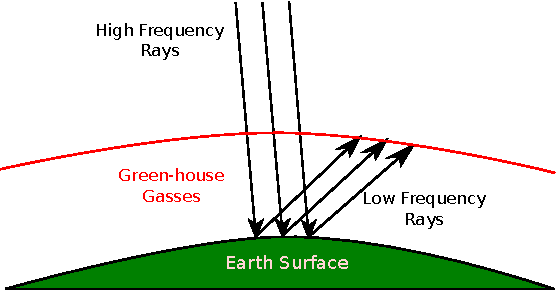
\includegraphics[width=0.65 \linewidth]{./figurer/G-H_gasses} 
  %
  \caption{Green-house gases act like a blanket trapping the heat received from
the sun.}
  \label{fig:grHsGs}
%
\end{figure}

Human manipulations in the nature has led to approximately $100~\mbox{ppm}$ increase in carbon dioxide level in the atmosphere. Most scientists believe that we are already experiencing the global warming due to green house effects. The IPCC Second Assessment report states that the observed warming trend since the late $19^{th}$ century is unlikely to be entirely natural in origin and is partly due to anthropogenic causes \cite{change1995ipcc}. 

Carbon capture and storage (CCS) has got a major attention in the industry and the scientific communities. According to the International Energy Agency (IEA), the cost of mitigating climate change by $2050$ is estimated to be $70\%$ higher without implementing CCS \cite{iaeScenario}.

CCS is considered as an interim solution, because it is valid due to fossil fuel consumption, and the long term strategy of replacing fossil fuel with renewable energy will terminate the validity CCS. Therefore, initiating CCS has to be done in a reasonable fashion such that it does not slow down the research for renewable energy. Another concern regarding CCS is the acceleration of coal and fossil fuel consumption with the excuse of availability of CCS technology.

\begin{figure}
  \centering
  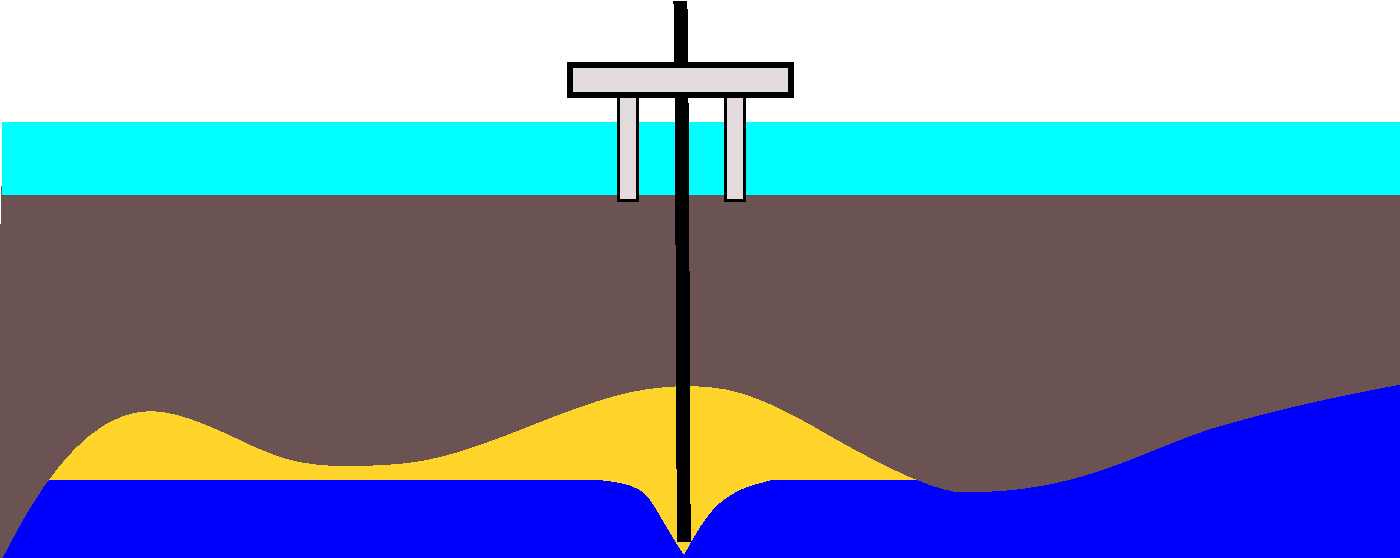
\includegraphics[width=0.65 \linewidth]{./figurer/platform} 
  \caption{Geological sequestration is a proposed solution for mitigating the
industrial $\mbox{CO}_2$ emissions.}
  \label{fig:platform}
%
\end{figure}


Sequestration of CO$_2$ at the ocean floor and also in deep underground aquifers are some of the options available for permanent storage of $\mbox{CO}_2$. Large availability of storage volumes and potential for almost permanent storage makes the geological sequestration an appropriate option (Figure \ref{fig:platform}). Nevertheless, this alternative is not free from economical, social and industrial concerns.  

In the last decades, the scientific community has been putting efforts into
convincing the public about the feasibility of these operations. A fair public acceptance must be based on social awareness. Any plan to increase the
acceptance level in a society starts by measuring the current knowledge level of that society. The EU has conducted a survey to assess the public awareness in $12$ European states. This survey is published in the recent Eurobarometer report in May $2011$. People's awareness and acceptance of climate change and its causes, and the methods to avoid or mitigate the problems, in particular the CCS technology, was examined in the survey. The majority of European participants are either fairly or very well informed about causes and consequences of climate change. However, the awareness of CCS in between the European respondents was low. Two third of the participants in the survey have had not heard at all about CCS. 

The same survey suggests that the overall trust in Europe in the sources of
information regarding  CCS is best in universities and other scientific
institutions. Governments are investing in research, not only to move toward
industrialization of CCS, but also to make it well received by public. This
highlights the importance of researching the storage of $\mbox{CO}_2$ and the
way it is needed both for industrial demands and social concerns.

\section{Modeling procedure}
\label{sec:MProcedure}

Predicting the fate of $\mbox{CO}_2$ storage involves identification and
quantification of the  relevant uncertainties and risk assessment process. The
procedure starts with a geological description and continues with modeling of
flow in geological formations. After constructing a deterministic flow model,
the stochastic nature of the problem is analyzed by studying the variation in
the model outcome due to uncertainties in the system. 

\begin{figure}
  \center
  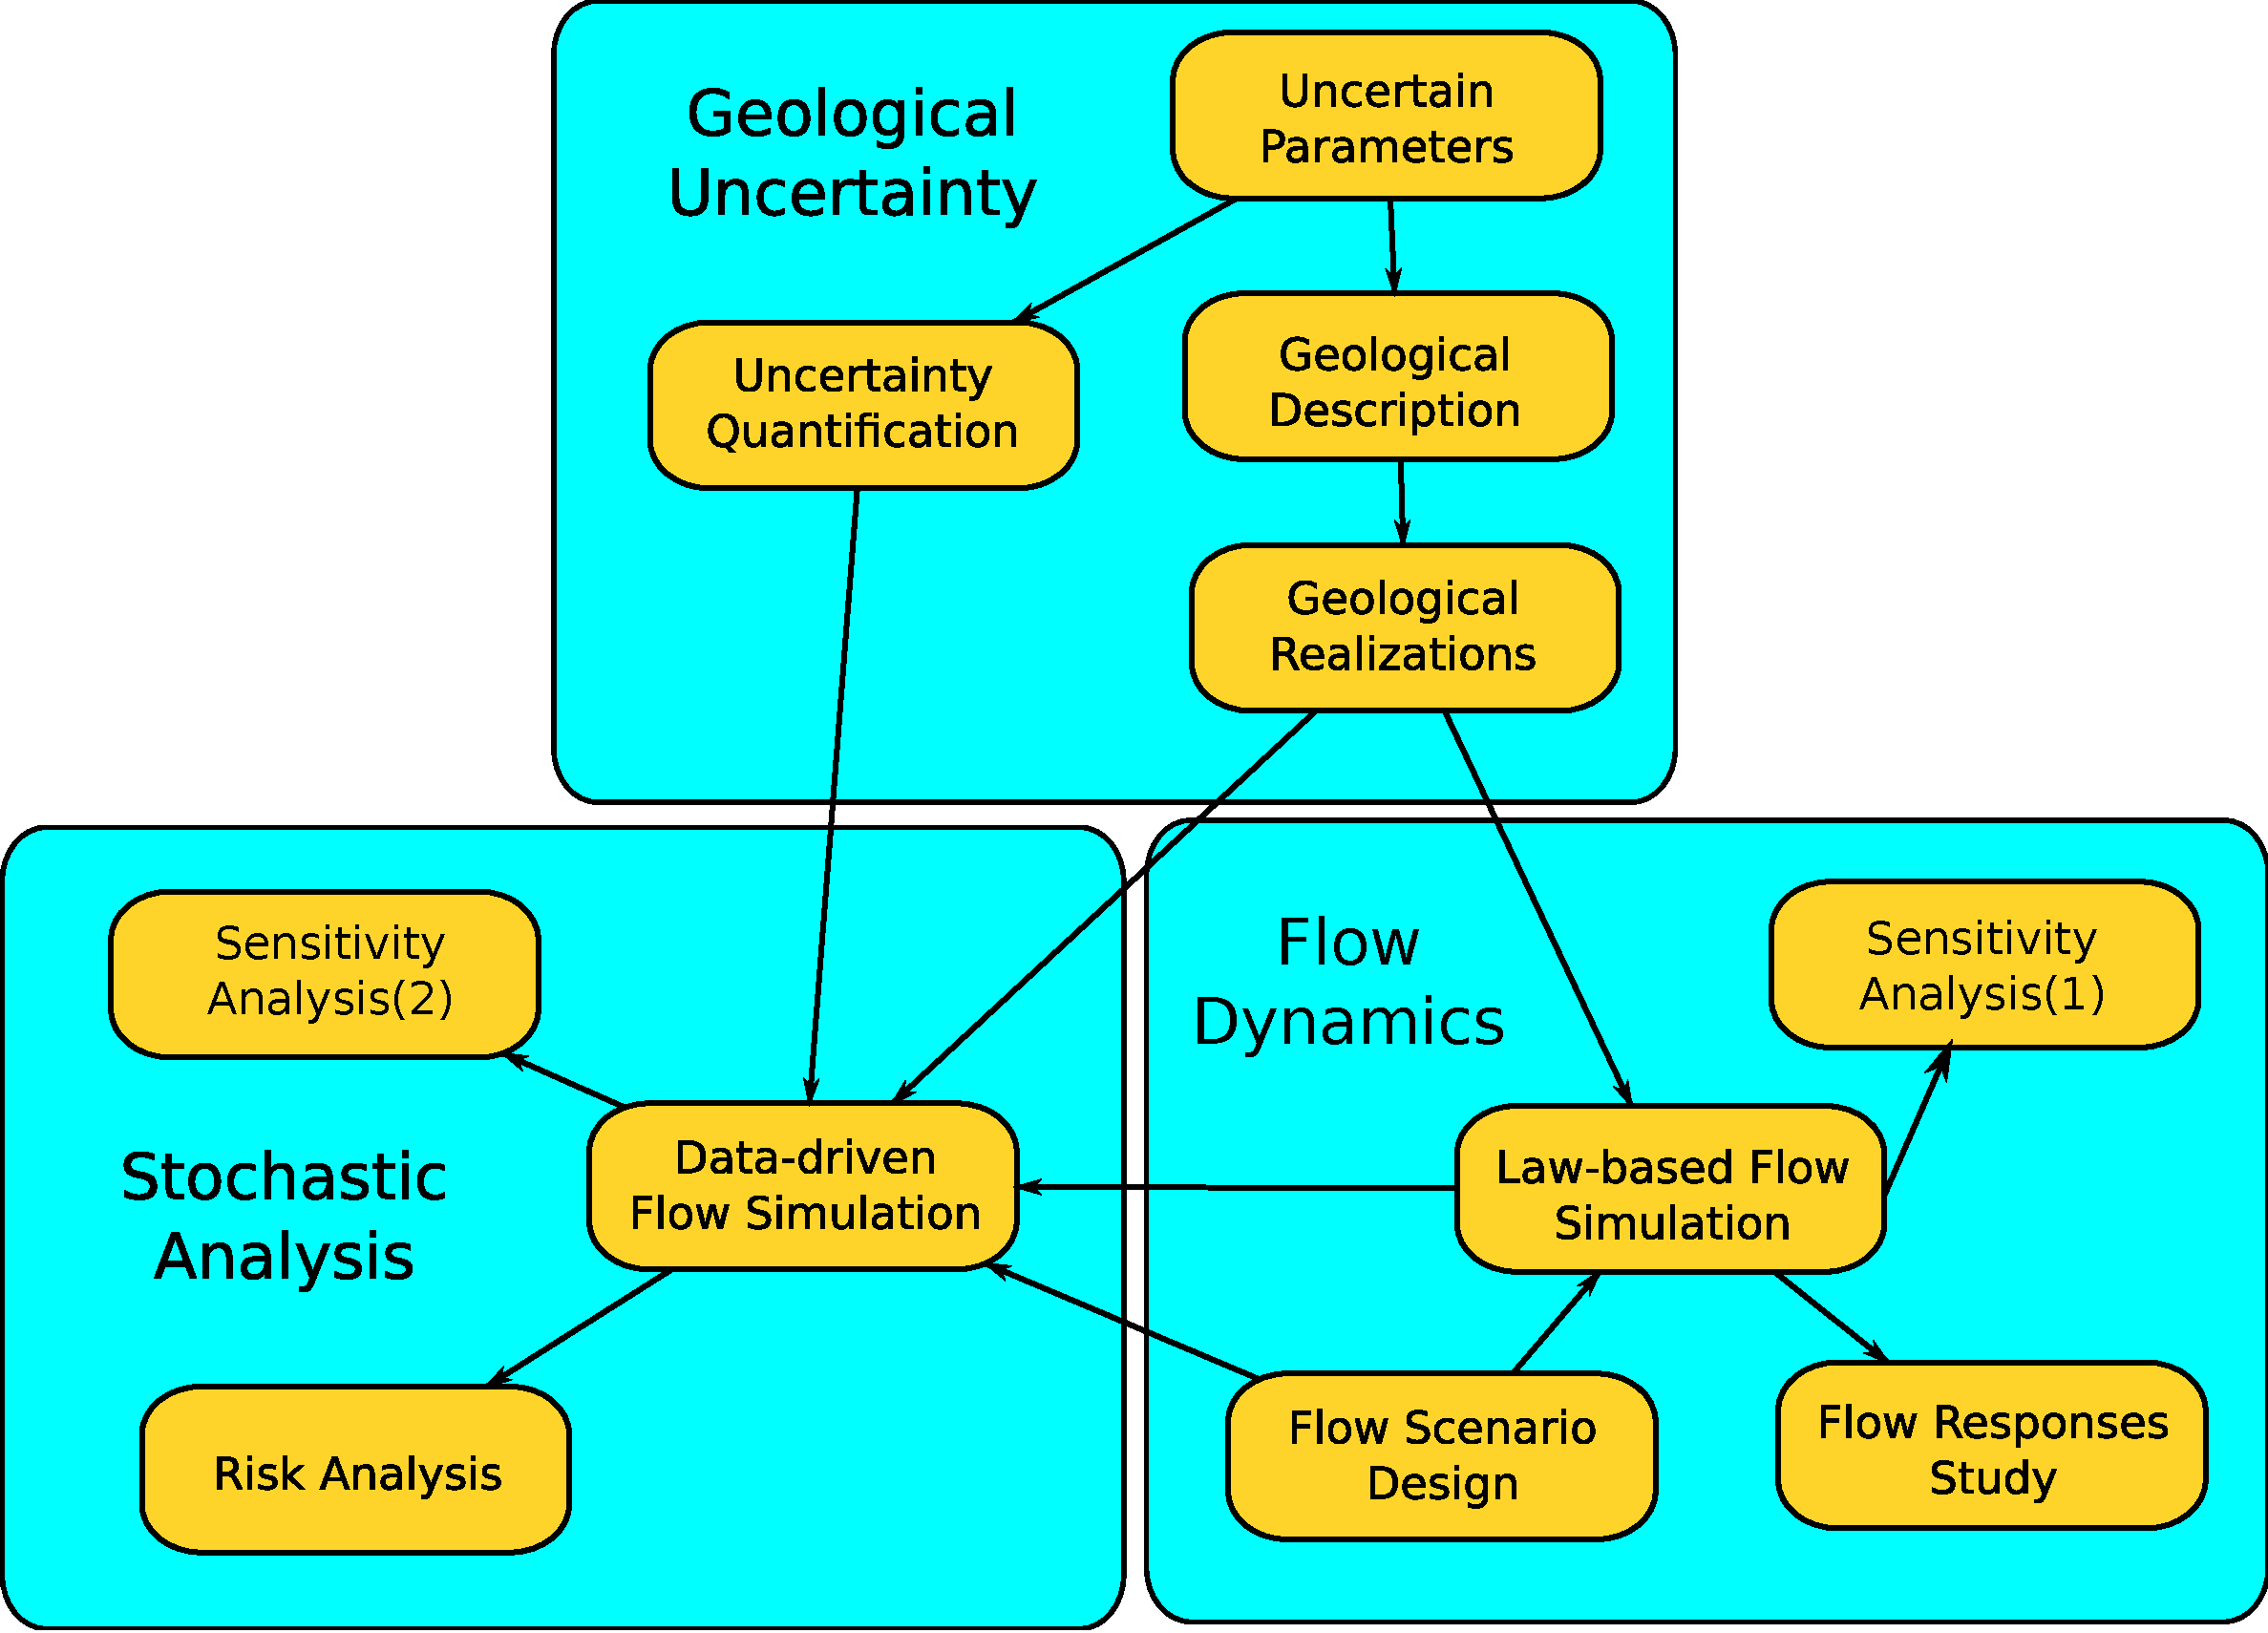
\includegraphics[width=0.95 \linewidth]{./figurer/prc3}
  %
  \caption{Modeling procedure diagram.}
  \label{fig:prc}
%
\end{figure}

Figure \ref{fig:prc} shows the modeling work-flow implemented in this thesis. The steps are categorized in three parts: geological uncertainty,
flow dynamics, and stochastic analysis. The relations between the steps are plotted by arrows in the flow-chart. In this section, we briefly describe each step. More details will follow in the next sections.

\textbf{Uncertain parameters:} In the first step, we identify the uncertain
parameters of the model  to study their influence in the modeling outcome. It is possible that our knowledge of model sensitivity to the parameters is limited. Then, in a conservative approach we choose a larger number of parameters and by doing a primary sensitivity analysis with a fast technique, we filter out the important parameters. Herein, the focus is on geological parameters that are determined to be the most influential sources of geological uncertainty for a shallow-marine environments \cite{howell2008sedimentological}.

\textbf{Uncertainty quantification:} After identification of the uncertain
geological parameters, we assign a likelihood to each of the parameters. It is hardly possible to have a unique likelihood template that applies to every
geological location. Thus, we note that probabilities of existence for an
uncertain geological feature can change from place to place. The uncertainty
enters the modeling in the form of parameter frequency histograms. The
conventional practice is to consider an analytical distribution function to be
assigned to the parameters. However, the sampling procedure normally ends in
scarce frequency histograms that are difficult to fit into a unique analytical
distribution function.

\textbf{Geological description:} Geological uncertainty study is normally done
by series of runs to measure the sensitivity of the model to the parameter
variations. Results are valid, only if the geology used in the work-flow is
representative of reality. The process of geological description results in a
large number of realizations to be used in the next steps of the study. Herein, we will use a set of equiprobable geological realizations of a shallow-marine reservoir.

\textbf{Flow scenario design:} Herein we define the initial and boundary
conditions of the $\mbox{CO}_2$ injection problem. Also, we specify the
injection scenarios. Possible simplifying physical assumptions will be taken
here. Each scenario is implemented for all geological realizations.

\textbf{Law-based flow modeling:} After defining the injection problem, we
simulate the flow dynamics in the chosen realizations. We use a two-phase flow model and a standard commercial simulator.


\textbf{Data-driven flow modeling:} Modeling the flow dynamics via formulations
of physical laws normally results in complicated equations with many degrees of
freedom. The computational cost of solving these equations is high, in
particular for uncertainty related studies that require
a large number of simulations to cover the variation in the uncertain
parameters. So called data-driven methods, are mathematical functions that are specified by correlating a set of unknown flow attributes to their corresponding uncertain parameter values. These methods need to be tuned by a law-based method before employment. Because these methods are designed to be only dependent on the uncertain parameters, they are normally low in computational costs. However, they may exhibit the pitfall of not following the physical rules and in some cases produce unrealistic results. 


\textbf{Flow responses study:} Once the simulation results are obtained from the
flow modeling procedure, it is possible to calculate the important flow
responses from simulation results. The fate of carbon storage and assessment of
the operations can be inferred from these responses. Storage capacity, injection rate, and leakage risk are evaluated from flow responses. Responses include pressure distribution over time. $\mbox{CO}_2$ plume development, and other quantities describing the dynamics of flow. 

\textbf{Sensitivity and risk analysis:} The sensitivity analysis is performed
in two ways: firstly by using three-dimensional, two-phase flow simulations on all realizations available for demonstrating the geological variability. In the second method, we employ an
approximating polynomial to perform global sensitivity analysis and
stochastic uncertainty studies. Using  the relatively fast data-driven method,
we perform a Monte-Carlo process on $10000$ simulation cases. 

\section{Uncertainty Sources}
\label{uncertaintySources}

Sources of uncertainty can exist in every part of the $\mbox{CO}_2$ storage modeling
process. Herein, we briefly describe each of the possible contributions to the
uncertainty in modeling within various parts.

\textbf{Uncertainty in physical modeling:} We might ignore some phenomena during
the physical modeling of $\mbox{CO}_2$ storage that can be influential in the
flow behavior. This might happen due to lack of awareness of the phenomena or by
underestimating the significance of it. For
example, we might ignore the heat exchange within the system, assuming that heat transfer does not play an important role in the flow performance. If some parameters in the modeling are sensitive to the heat and change by temperature variations, the assumption to ignore heat transfer effect can introduce considerable bias in the outcome of the modeling.

\textbf{Mathematical formulation and numerical approximation:} Modeling $\mbox{CO}_2$ injection and migration in a realistic geological
formation results in a complicated mathematical system that in most of the cases
can not be solved analytically. The numerical approach to approximate the
original mathematical system, normally introduces errors in approximation.
Mathematical analysis can help in estimating the error or its order, but it
might not be doable for complicated models.

A specified
physical problem can be formulated mathematically in more than one way. The
choice of primary unknowns to be found can change the mathematical form and
nature of the equations. Degrees of non-linearity and coupling between unknowns
in the equations can vary in different formulations. 



\textbf{Geological uncertainty:} The high costs of data acquisition and
technical
limitations introduce a huge amount of geological uncertainties in $\mbox{CO}_2$
storage modeling. The injected $\mbox{CO}_2$ may travel in a large spatial scale
and providing enough geological information and the medium attributes is a big
challenge.

\textbf{User introduced uncertainty:} These type of uncertainties are caused by
the errors introduced by a user for her/his biased choice of modeling tools and
interpretations of modeling results. 

\section{Geological modeling}
\label{sec:GeologicalModeling}

The central part of a successful $\mbox{CO}_2$ storage modeling is to
provide aquifer models that depict the geological heterogeneity in a
realistic manner. This requires having an inclusive understanding about model
sensitivity with respect to different geological parameters and quantifications
of geological uncertainty and its impacts on the process. 

The conventional practice of geological modeling includes using geostatistical
models. It is possible that two different heterogeneity patterns produce the
same geostatistical model, as discussed by Caers \cite{caers2002multiple}.
Therefore, a geostatistical model does not represent a unique reservoir image
and if we do not include additive information in the process, we might end-up
with an unrealistic heterogeneity
texture\cite{caers2002multiple,eaton2006importance}. The primary  attention in
our work has been on this issue and to provide a more realistic way of
geological uncertainty analysis for $\mbox{CO}_2$ sequestration by including
information of geological features and textures in the process. 


\subsection{Geological description}

Geological storage of \coo\ requires large accommodation of subsurface volumes. Only sedimentary basins, which hold relative large pore volumes, are generally suitable for this mean. However, not all sedimentary basins are similarly appropriate for \coo\ sequestration.

Convergent basins along active tectonic areas pose a higher risk of \coo\ leakage due to volcanism, earthquakes, and active faults. Divergent basins located on the stable lithosphere are much less prone to earthquakes or other catastrophic event that can lead to accidental releases of large \coo\ quantities. Therefore, specific considerations must be done in selecting site locations with respect to security of subsurface storage.

Sedimentary basins are composed of various lithological facies. Stratigraphic architecture and sandbody geometry control the capacity and effectiveness of \coo\ sequestration. As a result of various tectonic depositional and erosional process, low and high permeability rocks are accumulated on top of each other and can form stratigraphic flow-path leading to various directions and speed of subsurface flow. Three types of formations can be characterized: aquifers, aquitards, and aquicludes. 

Aquifers are high permeability strata that provide major beddings for flow transport. Good rock quality in continuous sandbodies allow for efficient \coo\ storage in an acceptable capacity volumes. Aquitards are made of low permeability strata that provide beddings with orders of magnitude slower flow than aquifers. Layers of aquifers and aquitards are formed by thick accumulation of sediments that undergo burial, compaction, lithification and uplift over millions of years. They can be covered by aquicludes, which are evaporative beds that are impervious to fluid flow. Typical seal rocks include, from most ductile to most brittle: salt, anhydrite, krogen-rich shales, dense mudstone, tightly cemented sandstones, anhydrite-filled dolomite, carbonate, or silica-cemented sandstones, and cherts.

Aquifer pressure is normally close to hydrostatic, because of the conductivity within the medium allows for pressure equilibrium over long time. High pressurized compartments can exist in highly sealed structures. The pressure of the sedimentary basin has a significant impact on its suitability for \coo\ storage \cite{bachu2000sequestration}. Trapping mechanism for \coo\ is in two main parts: stratigraphic and structural traps. Stratigraphic trapping  is primarily controlled by the geometry of depositional facies and sand body continuity. These factors control the permeability distribution within the medium that controls the efficiency of injection and storage of \coo. Structural heterogeneity factors include faults, folds, and fracture intensity. The dip angle of formation layers control the buoyancy forces that govern on \coo\ plume migrating along the conductive layers. Fractures can enhance the mobility of the plume and sealing faults can provide structural traps for long-term \coo\ storage. Anticline structures also can be permanent traps for stored \coo.

Depositional environment varies between fluvial to marine systems. The texture and degree of sandiness of beach deposits are functions of the shore profile, typically consisting of a gently sloping formation layering in a transition from near shore to deep offshore. Deposits range from sandy, coarse grain structure near the shore, to muddy, burrowed, fine grained sand in the lower off shore. High energy near the shore that is a result of interplay between wave, fluvial, and tidal forces, filters out the larger grains in the deposition.

Therefore, formations closer to the shore contain large continuous sand bodies that have good quality rock. This is the reason for shallow-marine systems to be appropriate traps for hydrocarbons and analogously, good candidates for \coo\ storage.

\begin{figure}
\begin{tabular}{cc}
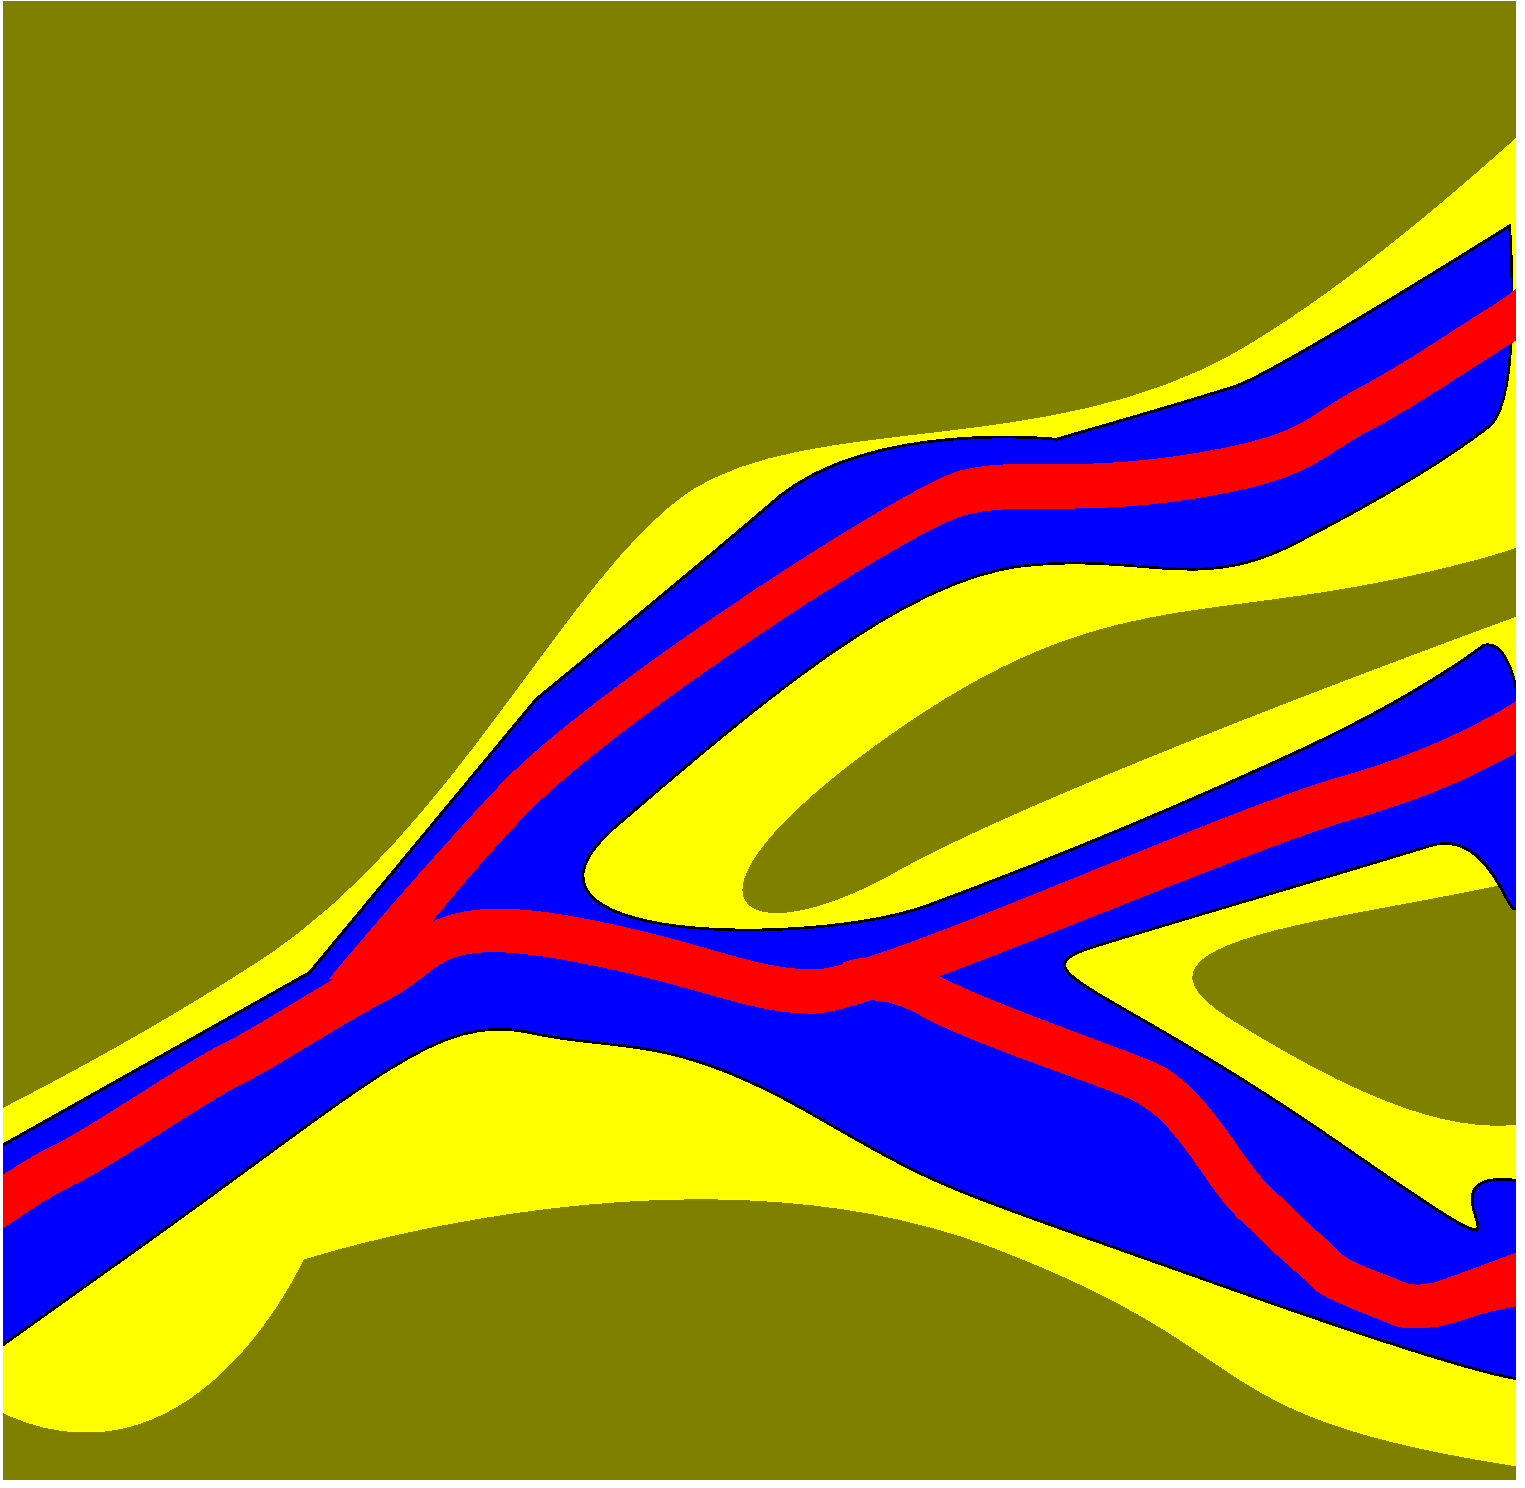
\includegraphics[width=0.3\textwidth]{./figurer/delta_fluvial}&
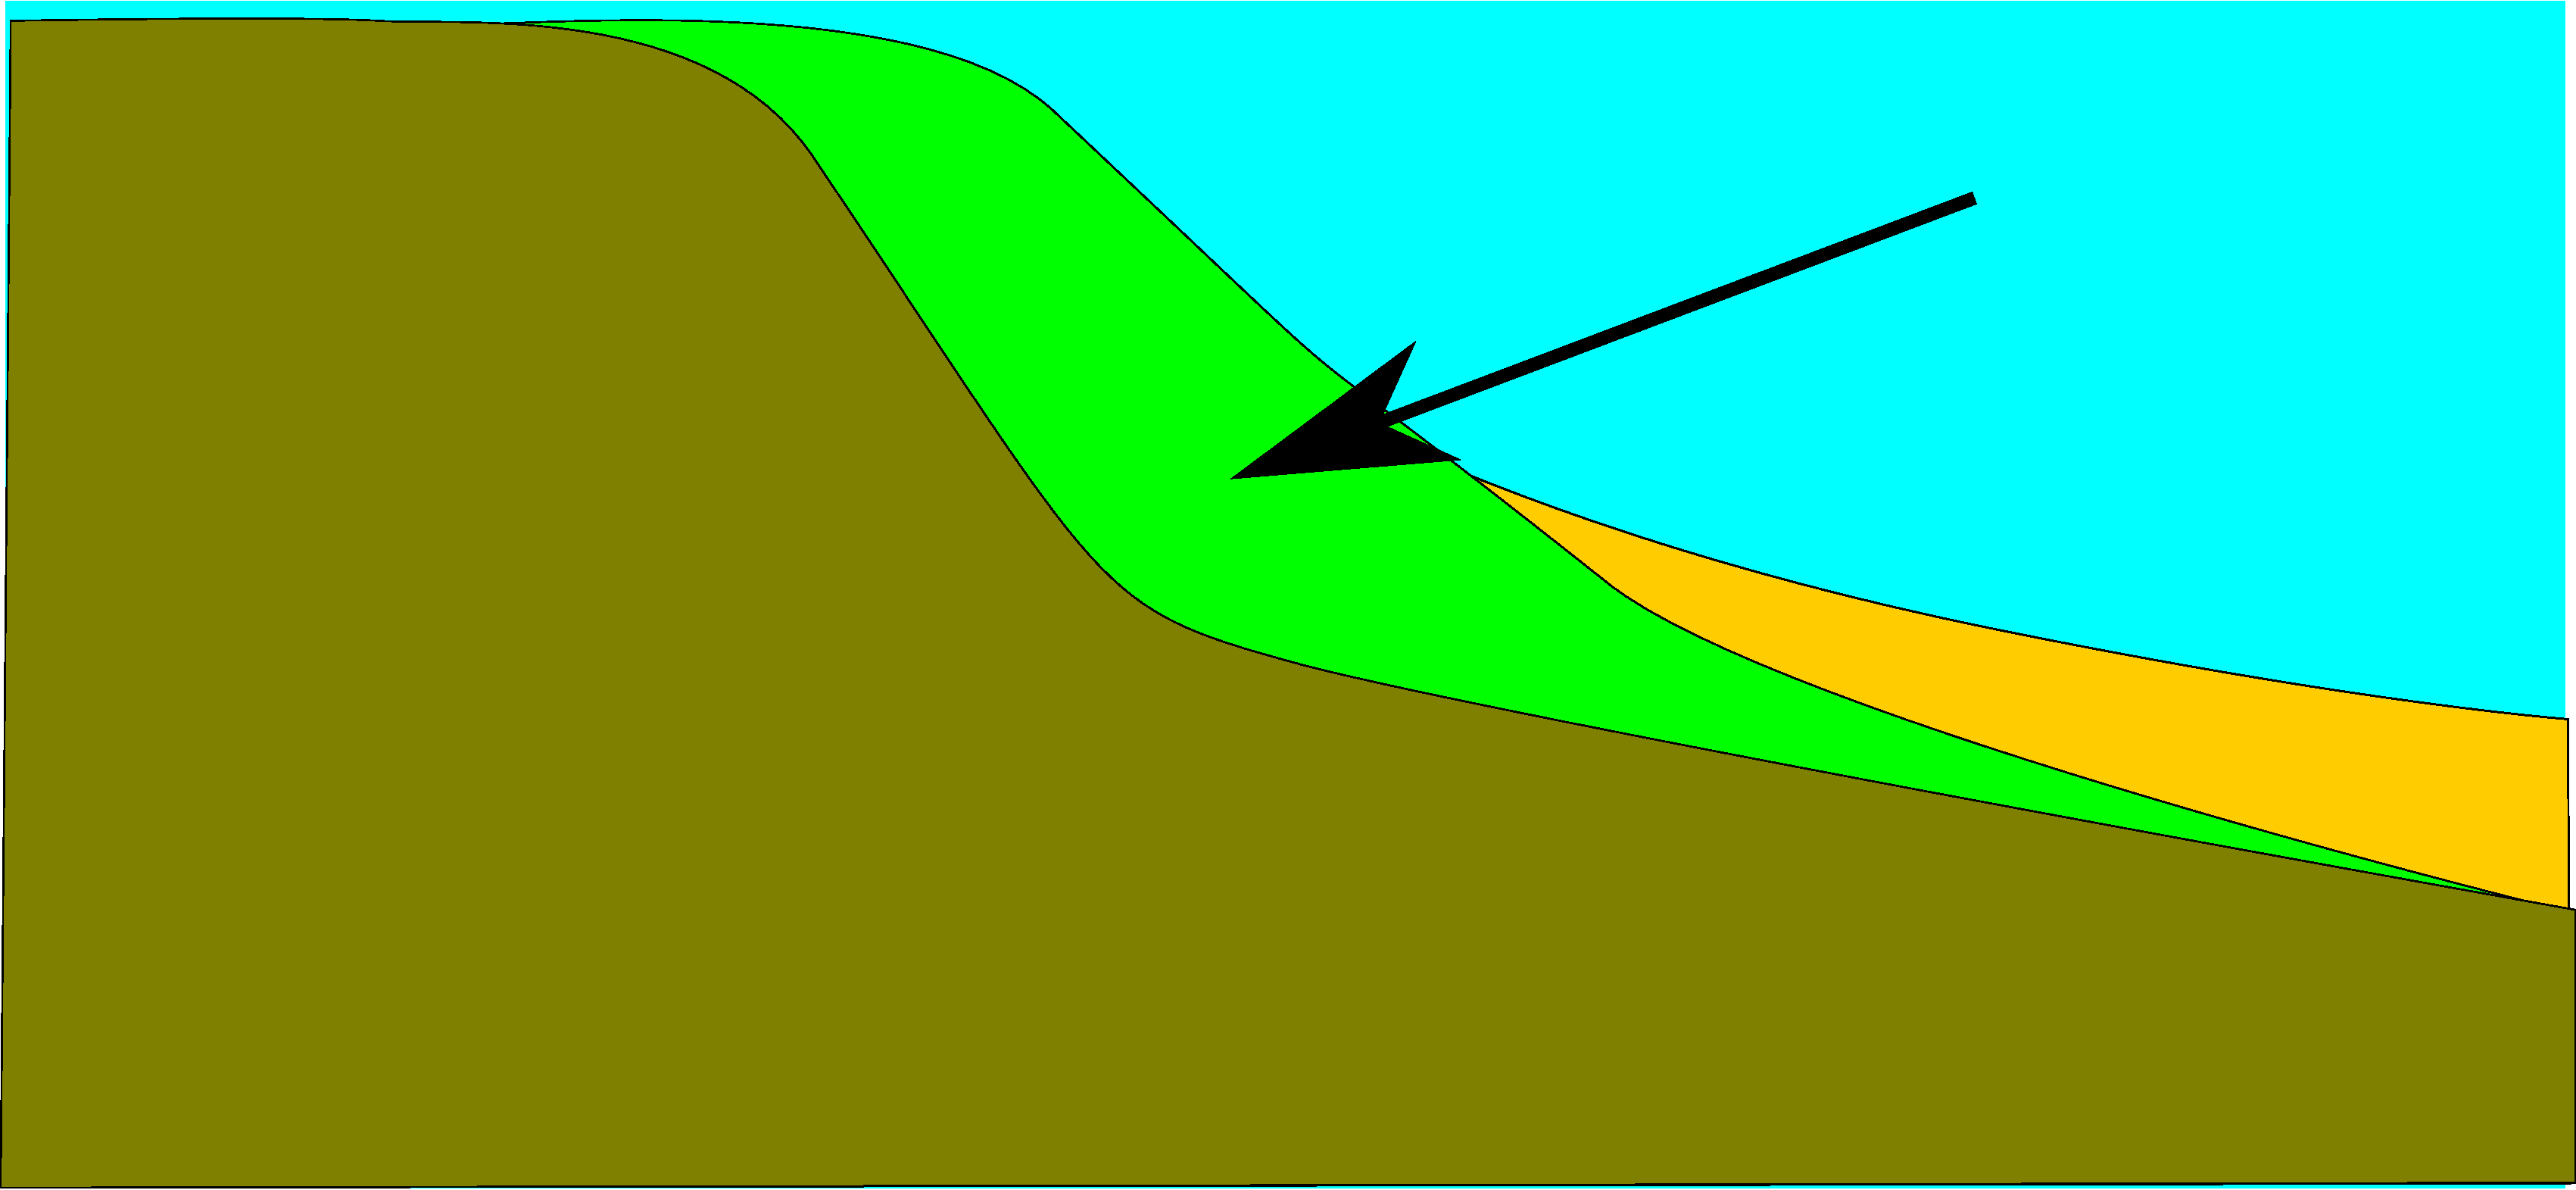
\includegraphics[width=0.65\textwidth]{./figurer/delta_beach}\\(a) Fluvial depositional system. &(b) Beach depositional system.
\end{tabular}
\caption{Heterogeneities in fluvial and beach depositions. Arrow in Figure (b) shows that the deposition mass is less heterogeneous than the fluvial systems.}
\label{fig:delta}
\end{figure}

The beach facies normally are homogeneous rocks with internal heterogeneity due to tidal systems. In contrast, mixed-load fluvial deposits that contain both mud and sand are more heterogeneous than beach systems. The presence of numerous mud drapes as a result of periodic floods, serve as barriers to fluid flow. Heterogeneity in the fluvial systems exist on multiple scales, from small-scale variations of rock type near the river bed, to the large-scale heterogeneity in fluvial channel-fill sandstones and over-bank deposits. Heterogeneity also occurs within these systems in the form of muddy abandoned channel-fill deposits.

In theory, we prefer a medium that allows for more lateral movement to overcome the buoyancy bypassing of the flow. Heterogeneity in the vertical direction, such as shale inter-bed barriers can serve for this and disperse the flow in the lateral direction. Structural heterogeneities can have a similar impact. In addition, splitting a large plume into smaller plumes lowers the risk of leakage of huge \coo\ amounts via potential breakings in the integrity of the sealing barriers, or abandoned wells.

\coo\ injectivity is related to sequestration capacity and effectiveness, and can be defined by the conductive cross-sectional area. Stratigraphic factors that enhance injectivity are high permeability and injection interval thickness. In addition, the lateral permeability architecture can influence the injectivity quality. The lower the injectivity is, the higher will be the pressure buildup in the medium due to injection.

%\begin{figure}
%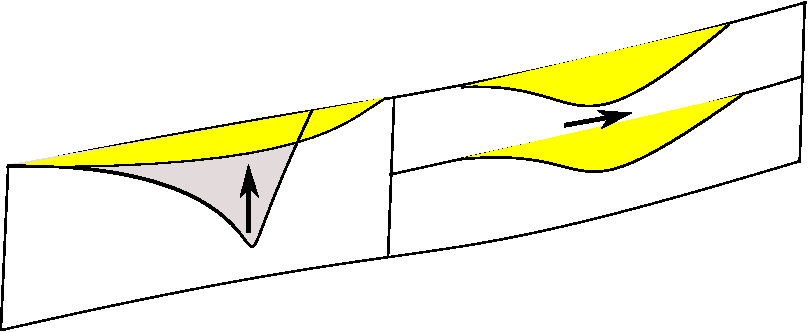
\includegraphics[width=0.7\linewidth]{./figurer/lateral_vertical}
%\caption{Heterogeneities in the vertical and lateral direction impacts the %flow direction, sweep efficiency and \coo\ plume size.}
%\label{}
%\end{figure}

Over the last two decades, there have been a large number of studies concerning the subsurface storage of \coo. Several authors investigate the efficiency of geological \coo\ storage based on regional data in a specific site location.

A case study from the Texas Gulf Coast \cite{hovorka2004impact} investigates the sequestration capacity and efficiency in accordance to the geological heterogeneity. The study performs a site-scale assessment of brine aquifers for geological \coo\ sequestration. Injection is considered in the Frio formation which is a sandstone-rich, high quality, overlain by a thick, regionally extensive shale in the upper Texas Gulf Coast. Migration of \coo\ during injection (20 years), and post-injection (40 years) is studied in different geological realizations. The heterogeneity represented by stochastic modeling of geological sediment. Structural heterogeneity is modeled by layers dip angle and faults at different locations. Six models are made based on regional available geological information. The study shows that in a homogeneous rock volume, \coo\ flow paths are dominated by buoyancy, bypassing much of the lateral rock volume. If the permeable rock is inter-bedded with multiple low permeability layers, the flow paths are dispersed, enhancing the lateral movements of  \coo\ and allowing for larger percentage of contact with rock volume. The study suggests that dip angle enhances buoyancy forces and decreases storage capacity, while compartmentalization by faulting appears to increase sequestration capacity at the cost of increased pressure, and consequently, increased risk of \coo\ leakage.

A number of pilot sites are established worldwide to test the large-scale injection of \coo\ in the subsurface formation. The In Salah project \cite{riddiford2004monitoring} in Algeria is an industrial-scale injection project into a fracture-influenced, matrix-dominated sandstone formation. The reservoir matrix comprises tidal deltaic sandstone. The project benefits from relatively high level of data acquisition: wireline and LWD well logs, image logs and production and geophysical monitoring \cite{riddiford2004monitoring}. In addition, the most valuable monitoring method has been the use of satellite airborne radar above the injection well. Also, chemical tracers are used in the injected \coo\ to differentiate the natural \coo\ in place from the injected volumes, when the \coo\ breaks through other wells. The detailed analysis highlights the geological controls on the movement and dispersion of \coo\ plumes. The injection is performed via a horizontal well perpendicular to the geomechanical stress field and the faults present in the domain. This, along with the fracture network, enhance the plume migration- about three times faster than the flow in a homogeneous domain. Results from In Salah illustrate the value of reducing geological uncertainty by employing sufficient logging tools and monitoring techniques. 

The \coo-SINK project at Ketzin Germany \cite{forster2006baseline} is another pilot site for practicing subsurface \coo\ injection. The injection is performed in the Stuttgart formation that is geologically heterogeneous within an anticline structure. The Stuttgart formation is made of sandy channel facies of good rock quality alternate with muddy flood-plain-facies. A thick cap-rock section covers the Stuttgart formation.

Practically, including all details of every scale into a flow simulation model is impossible. Various simplifications have been made to account for heterogeneities in modeling. Some earlier studies consider two dimensional modeling, with homogeneous or geostatistically populated permeabilities. The study in \cite{lindeberg1997escape} simulates an escape rate of \coo\ in a homogeneous medium similar to Utsira formation in Norway. By changing the horizontal permeability, they demonstrate that most of the injected \coo\ volume accumulates in a fine layer beneath the cap-rock due to buoyancy forces in the long-term \coo\ migration process. However, this study assumes no vertical heterogeneities. A layered heterogeneity is examined in \cite{van1995co}. They used a log normal distribution of permeability in a simplified two dimensional grid to account for viscous and gravity forces. Results suggest that the sweep efficiency of \coo\ in the porous medium is low, and heterogeneity, in particular the vertical transmissibility, can have a big impact on the storage efficiency. 

To examine the impact that the geological heterogeneity degree can have on the $\mbox{CO}_2$ sequestration modeling, \cite{flett2007heterogeneous} constructed a suite of three-dimensional simulation models, with varying net to gross ratios. A radial variogram, with a shale length of 300 m, was used to
populate five models of varying degrees of net-sand-to-gross-shale ratios. The models were up-scaled, using flow-based methods, to make the computation feasible. The study concludes that formations containing shale barriers are effective in containing an injected CO2 plume within the formation and that heterogeneity serves to limit the reliance of the formation seal as the only mechanism for containment.

\subsection{Geological parameters}

From the flow modeling perspective, sources of geological uncertainty can
manifest themselves in the rock parameters that go in the flow equation such as permeability and porosity. However, to represent the geological uncertainty, it is not enough to randomize these parameters. This approach might work in simple geological models, but it can fail to give plausible results for the realistic heterogeneous problems with uncertain structural and depositional descriptions.

In response to the EU priorities of reducing time to first oil and of improving
overall hydrocarbon recovery efficiency, the interdisciplinary SAIGUP study was
initiated to increase the understanding of the influence of geological
uncertainties in oil field recoveries. SAIGUP stands for 'sensitivity analysis
of the impact of geological uncertainties on production forecasting in clastic
hydrocarbon reservoirs'. The context in SAIGUP is defined for shallow-marine
depositional systems. The main objective of the SAIGUP project has been to
perform a quantitative sensitivity analysis to measure the impact of
sedimentological and structural variations within geological descriptions on 
oilfield recovery estimates
\cite{howell2008sedimentological,manzocchi2008sensitivity,matthews2008assessing}. Herein, we will use six different rock types  to investigate the impact of geological heterogeneities on \coo\ sequestration.  The rock properties within each facies are populated based on real data. Variations are considered in a horizontal-vertical matrix in three levels of heterogeneities, low, medium, and high, as illustrated in Figure \ref{fig:stratMat}. The design focused on special considerations. For example, making complex enough heterogeneities to be a plausible representative of realistic models, and producing large enough number of realizations with sufficient overlapping to be able to perform a quantitative sensitivity analysis.

Sedimentological variability is modeled in small and large scales and combined
to provide realistic variations of reservoir heterogeneities.  All models are considered in a progradational sedimentary environment. A regular grid is used for all of the realizations in two gridding resolutions, fine and coarse, and the total bulk volume is the same in all cases. Each geological realization contains about $1.5$ million cells in the fine model. Figure \ref{fig:finAct} shows the fine grid model for a selected realization with medium level of heterogeneity. A major fault in the model breaks the structure and makes large vertical depth difference in the two parts of the model (from about $1500$ m to $3000$ m).  Thickness of the model is much smaller than these depth differences. To make it easier to see the property variations on the grid in the vertical direction, we map the properties on a flat uniform geometry (Figure \ref{fig:finUnf}).

Figure \ref{fig:facies} shows the spatial distribution of the six modelled facies in the selected realization, and Figure \ref{fig:kxh} shows the histogram of lateral transmissibility within each facies and the total model in the logarithm scale. Each facies is modeled separately in some levels of upscaling starting from the lamina scales, before populating on the fine grid. Flow based upscaling techniques are used, and the suitability of the methods depends on the balance of
forces. When the medium is conductive due to high permeability, the viscous dominated steady state method is used. In the rocks with lower transmissibility where the capillary forces are dominant, the capillary equilibrium is assumed \cite{manzocchi2008sensitivity}.

On the last step, the fine populated grid is mapped on to the coarse grid that is to be used for the flow solver. Since the grid size in the fine model is too expensive computationally for flow simulations, the lateral dimension is doubled in each cell while every four layers are lumped into one layer in the vertical direction. Figure \ref{fig:upsat} shows the top view of lateral transmissibility in logarithmic scale for four consecutive layers of a selected case, and their corresponding upscaled layer in the coarse grid. Table \ref{tab:grids} shows the grid specifications in the coarse and fine SAIGUP models.

A detailed discussion about the upscaling the Sedimentological and structural parameters for SAIGUP simulation models can be found at \cite{manzocchi2008sensitivity}.

\begin{table}[tbp]
  \centering
  \caption{Grid specifications for fine and coarse scales in the SAIGUP modeling process.}
  \label{tab:grids}
  \small
  \medskip\renewcommand{\arraystretch}{1.2}
  \begin{tabular}{|p{.35\linewidth}|p{.15\linewidth}|p{.15\linewidth}|}
    \hline
    Parameter &  Fine Scale& Coarse Scale\\ \hline
    Number of cells in the x direction & $80$&$40$\\% \hline
    Number of cells in the y direction & $240$&$120$\\% \hline
    Number of cells in the z direction & $80$&$20$\\% \hline
    Number of total cells & $1,500,000$&$96,000$\\% \hline
    Number of active cells& $1,500,000$&$79,000$\\% \hline
	Model x dimension& $3~km$&$3~km$\\% \hline
	Model y dimension& $9~km$&$9~km$\\% \hline	
	Model z dimension& $80~m$&$80~m$\\% \hline	
    \hline
  \end{tabular}\renewcommand{\arraystretch}{1}
\end{table}

\begin{figure}
\centering
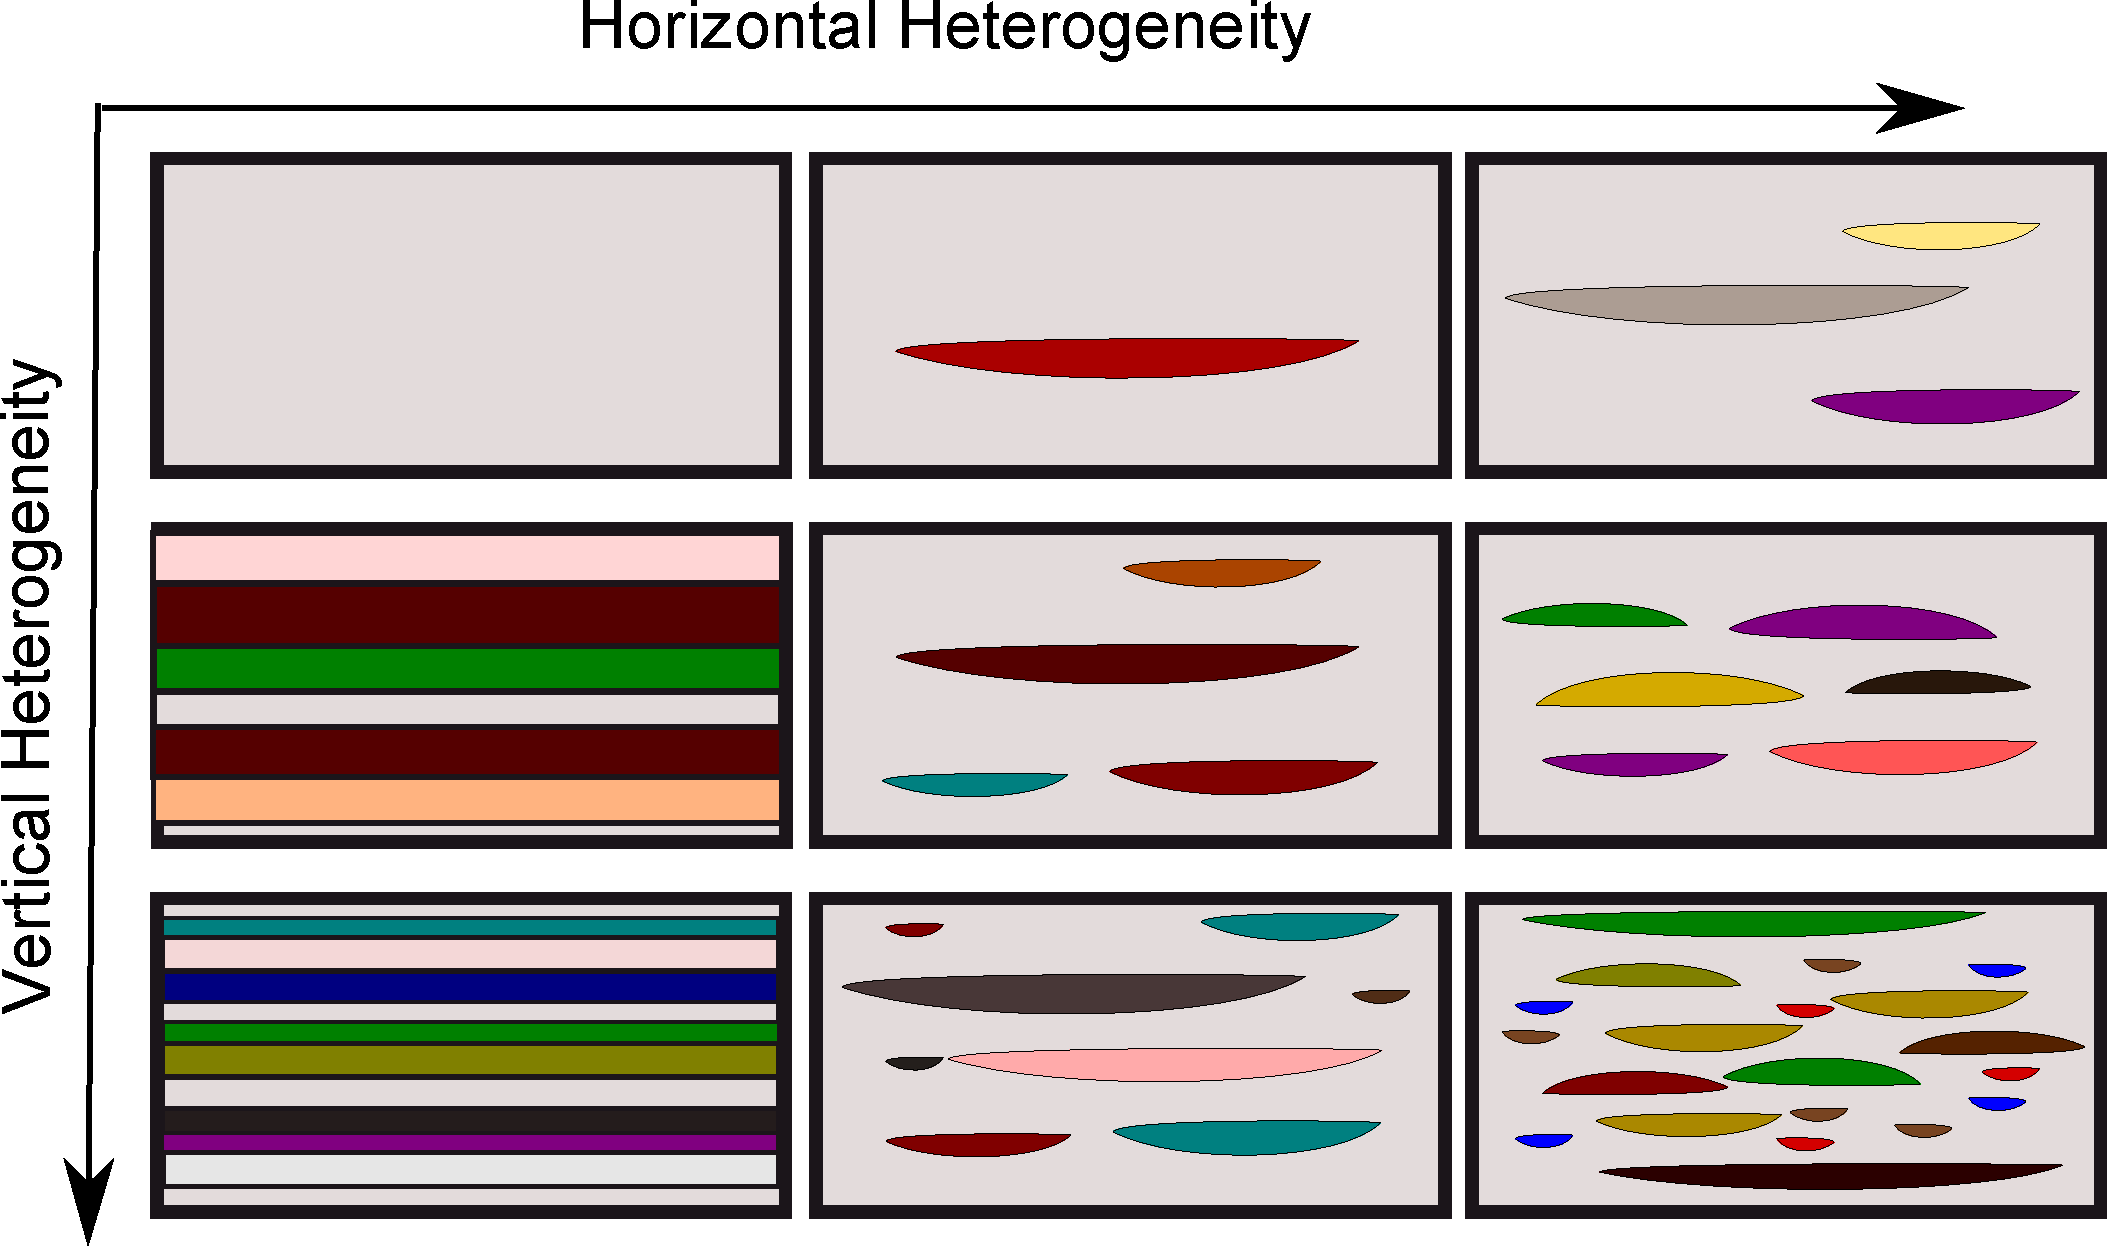
\includegraphics[width=\linewidth]{./figurer/stratMatrix}
\caption{Stratigraphic heterogeneity levels in lateral and vertical directions. Modified from \cite{manzocchi2008sensitivity}.}
\label{fig:stratMat}
\end{figure}

\begin{figure}
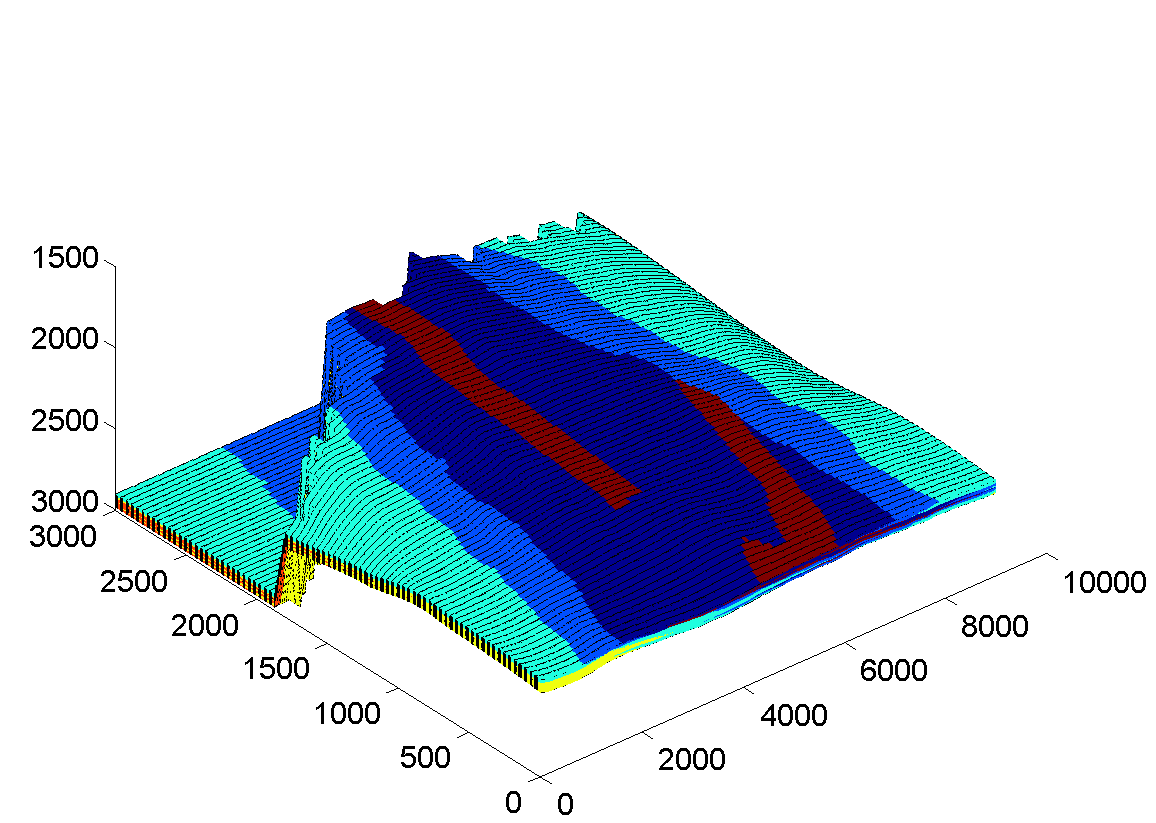
\includegraphics[width=0.8\linewidth,natwidth=555bp,natheight=395bp]{./figurer/fineSat_Perspective_actual.pdf}
\caption{Unfaulted fine grid perspective view. Colors depict rock types, see Figures \ref{fig:finUnf} and \ref{fig:facies}.}
\label{fig:finAct}
\end{figure}

\begin{figure}
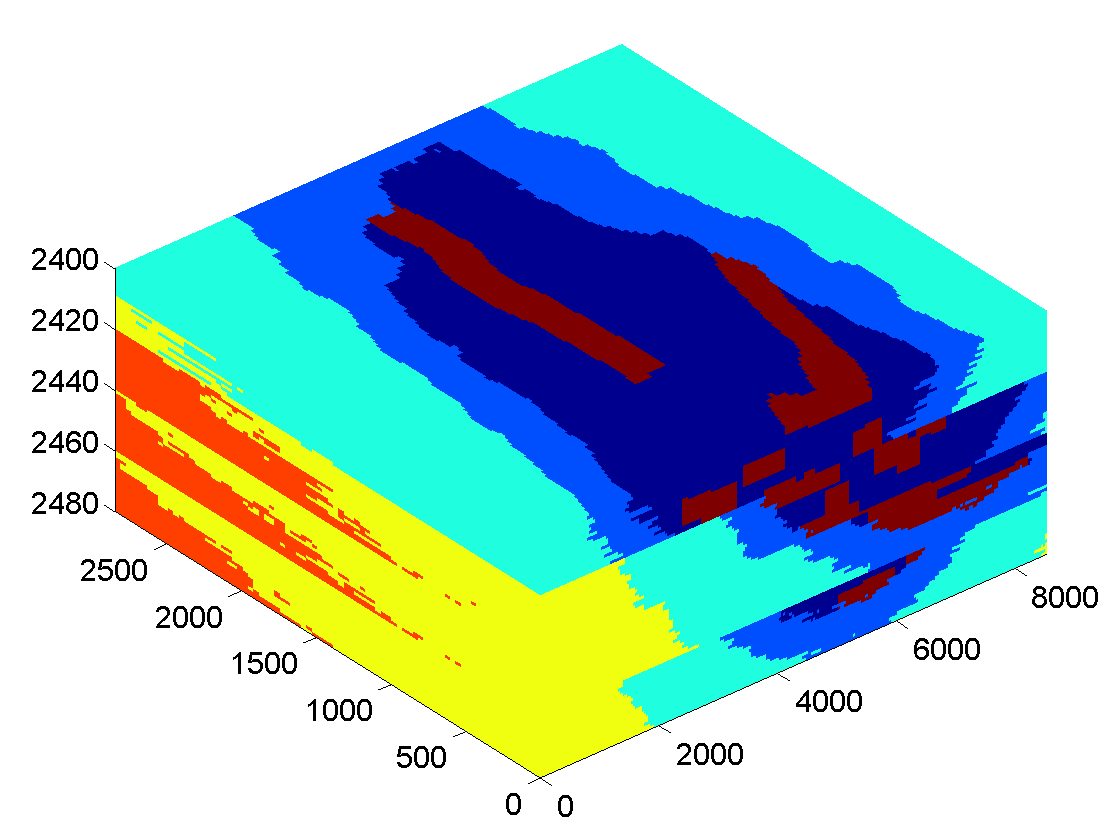
\includegraphics[width=0.8 \linewidth,natwidth=532bp,natheight=396bp]{./figurer/fineSat_Perspective_uniform.pdf}
\caption{Perspective view of the rock type variations for a selected case mapped on a uniform grid.}
\label{fig:finUnf}
\end{figure}

\begin{figure}
\begin{tabular}{ccc}
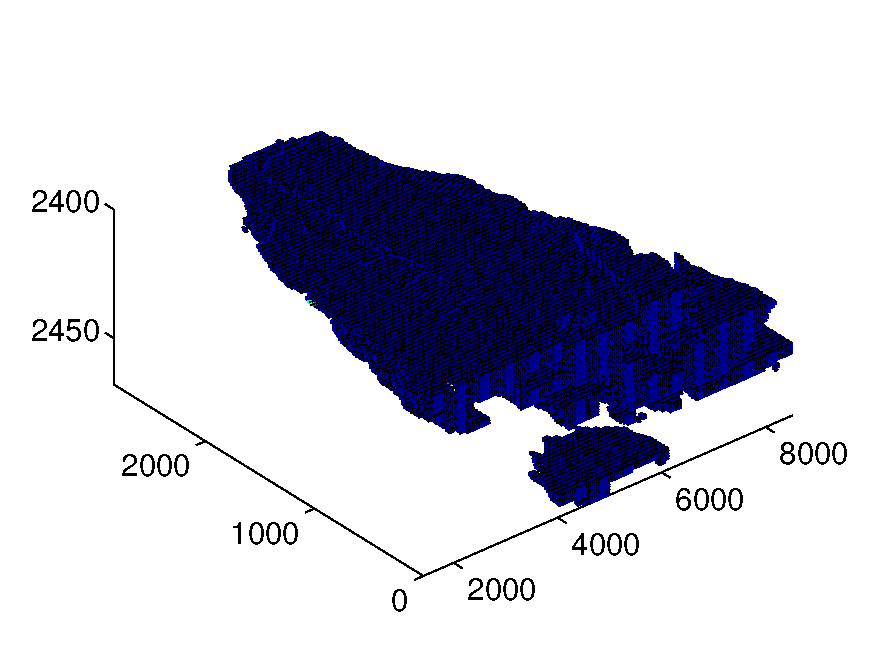
\includegraphics[width=0.3 \linewidth,natwidth=542bp,natheight=401bp]{./figurer/facies_1.pdf}&
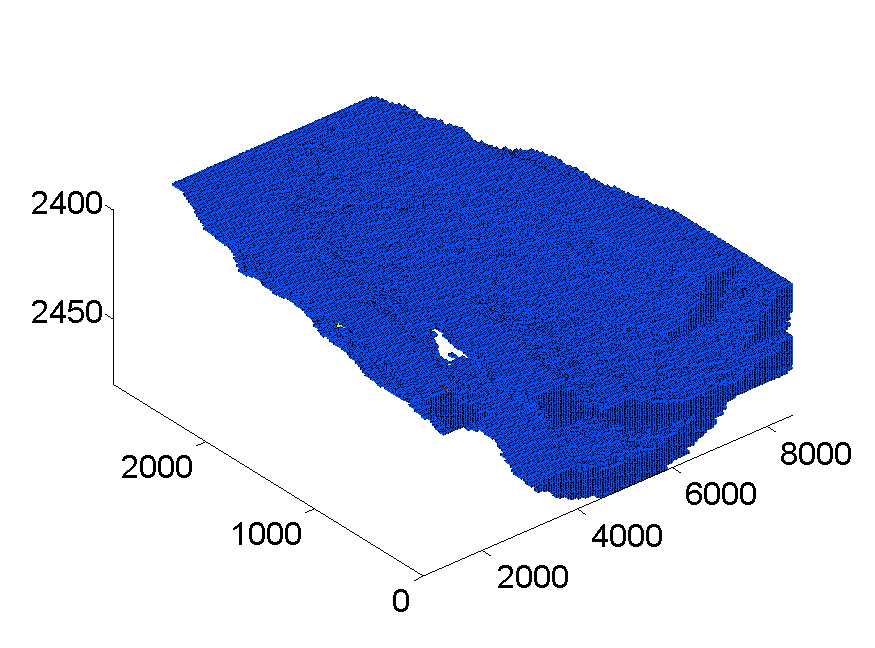
\includegraphics[width=0.3 \linewidth,natwidth=524bp,natheight=397bp]{./figurer/facies_2.pdf}&
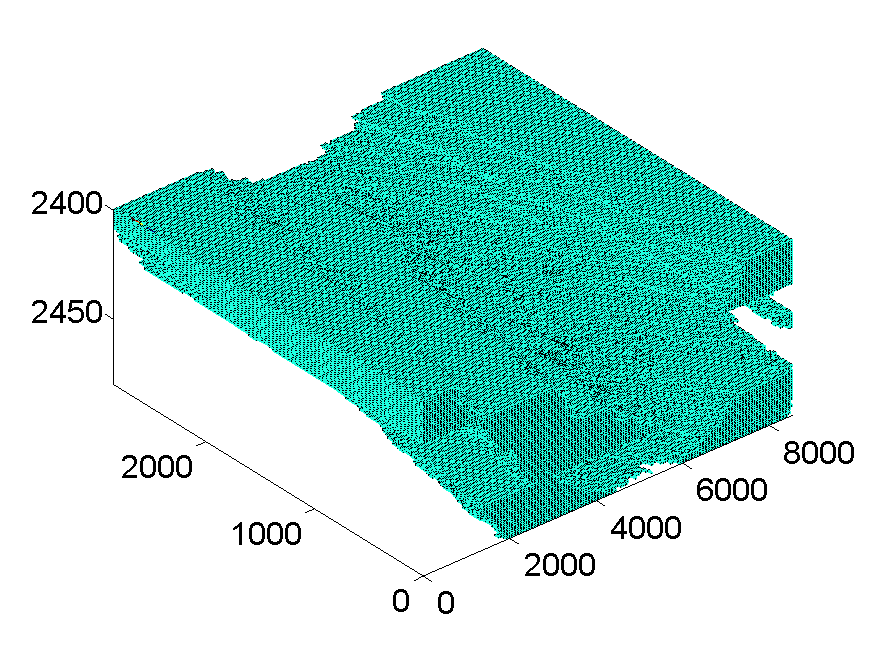
\includegraphics[width=0.3 \linewidth,natwidth=524bp,natheight=397bp]{./figurer/facies_3.pdf}\\(a) Coastal Plain&(b) Lower Shoreface&(c) Upper Shoreface\\
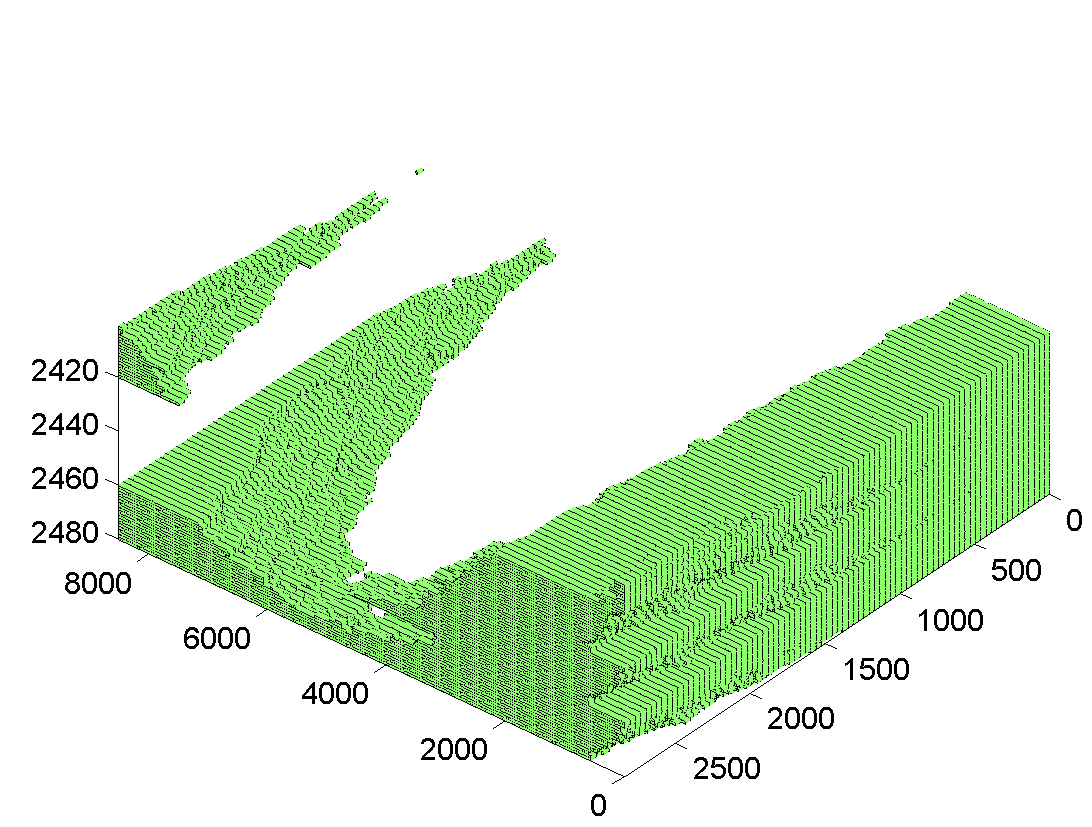
\includegraphics[width=0.3 \linewidth,natwidth=524bp,natheight=397bp]{./figurer/facies_4.pdf}&
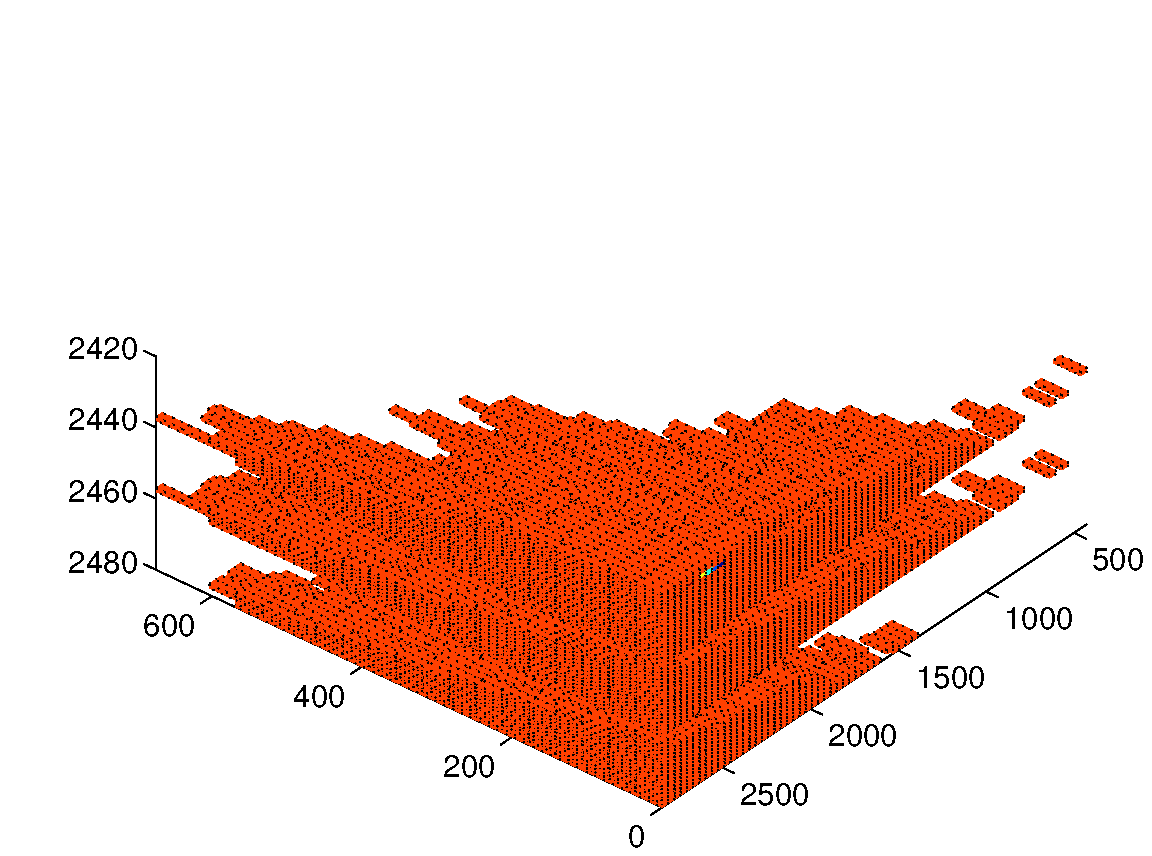
\includegraphics[width=0.3 \linewidth,natwidth=553bp,natheight=411bp]{./figurer/facies_5.pdf}&
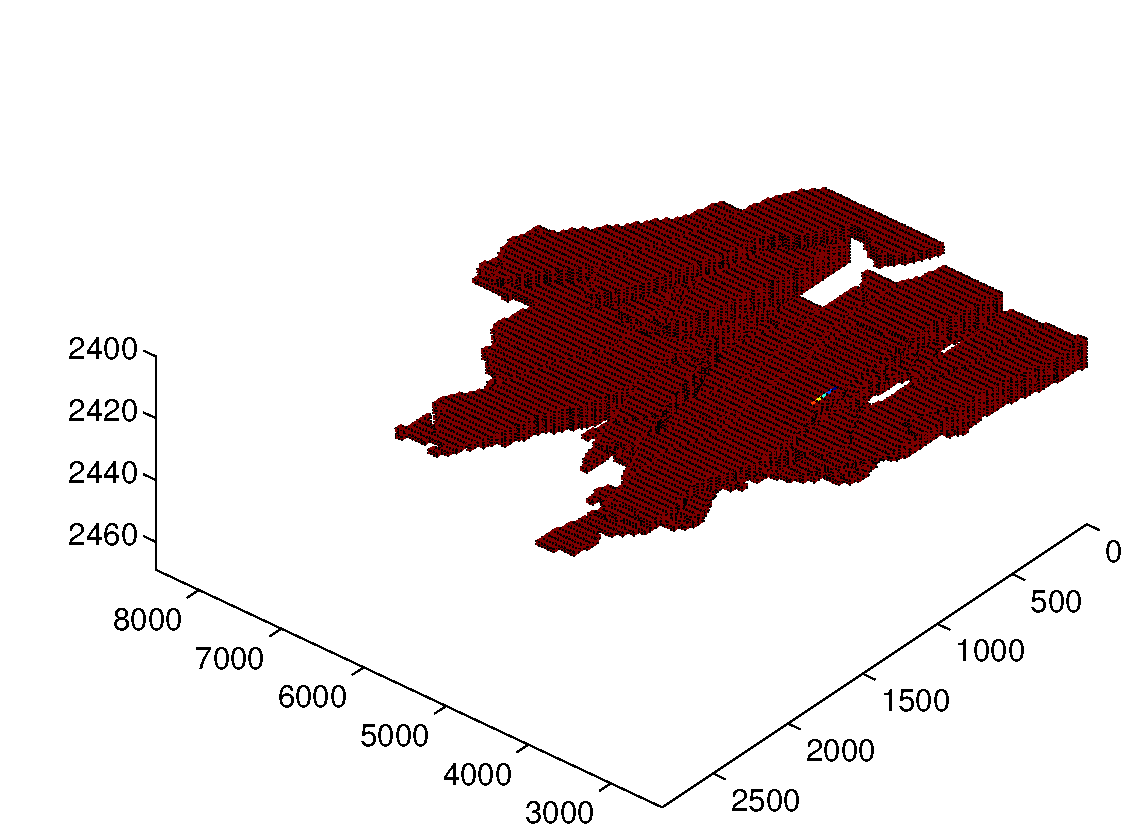
\includegraphics[width=0.3 \linewidth,natwidth=542bp,natheight=399bp]{./figurer/facies_6.pdf}\\(d) Offshore Transition&(e) Offshore&(f) Channels
\end{tabular}
\caption{Six different rock types used in modeling the stratigraphic heterogeneities. Compare to Figure \ref{fig:finUnf}}.
\label{fig:facies}
\end{figure}

\begin{figure}
\begin{tabular}{ccc}
\includegraphics[width=0.3 \linewidth,natwidth=504bp,natheight=385bp]{./figurer/kxh_1.pdf}&
\includegraphics[width=0.3 \linewidth,natwidth=508bp,natheight=385bp]{./figurer/kxh_2.pdf}&
\includegraphics[width=0.3 \linewidth,natwidth=474bp,natheight=399bp]{./figurer/kxh_3.pdf}\\(a) Coastal Plain&(b) Lower Shoreface&(c) Upper Shoreface\\
\includegraphics[width=0.3 \linewidth,natwidth=512bp,natheight=385bp]{./figurer/kxh_4.pdf}&
\includegraphics[width=0.3 \linewidth,natwidth=478bp,natheight=385bp]{./figurer/kxh_5.pdf}&
\includegraphics[width=0.3 \linewidth,natwidth=508bp,natheight=385bp]{./figurer/kxh_6.pdf}\\(d) Offshore Transition&(e) Offshore&(f) Channels\\
&\includegraphics[width=0.3 \linewidth,natwidth=462bp,natheight=399bp]{./figurer/kxh_All.pdf}&\\&(g) All facies&
\end{tabular}
\caption{Histogram of lateral transmissibility for different facies and the entire fine model for a selected case. Scales are logarithmic in units cP$.$m$^3$/day/bar.}
\label{fig:kxh}
\end{figure}

\begin{figure}
\begin{tabular}{c}
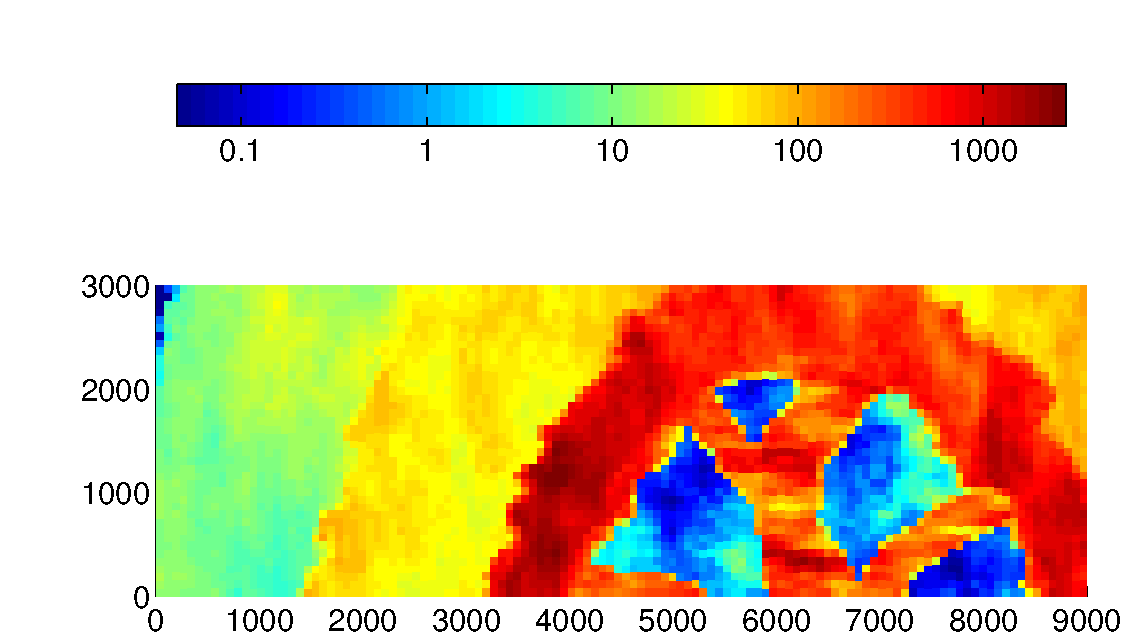
\includegraphics[trim=1.2cm 0cm 0cm 0cm, clip=true,width=0.8\linewidth]{./figurer/permxc}\\(a) Coarse grid.\\
\begin{minipage}{1\textwidth}
\begin{tabular}{cc}
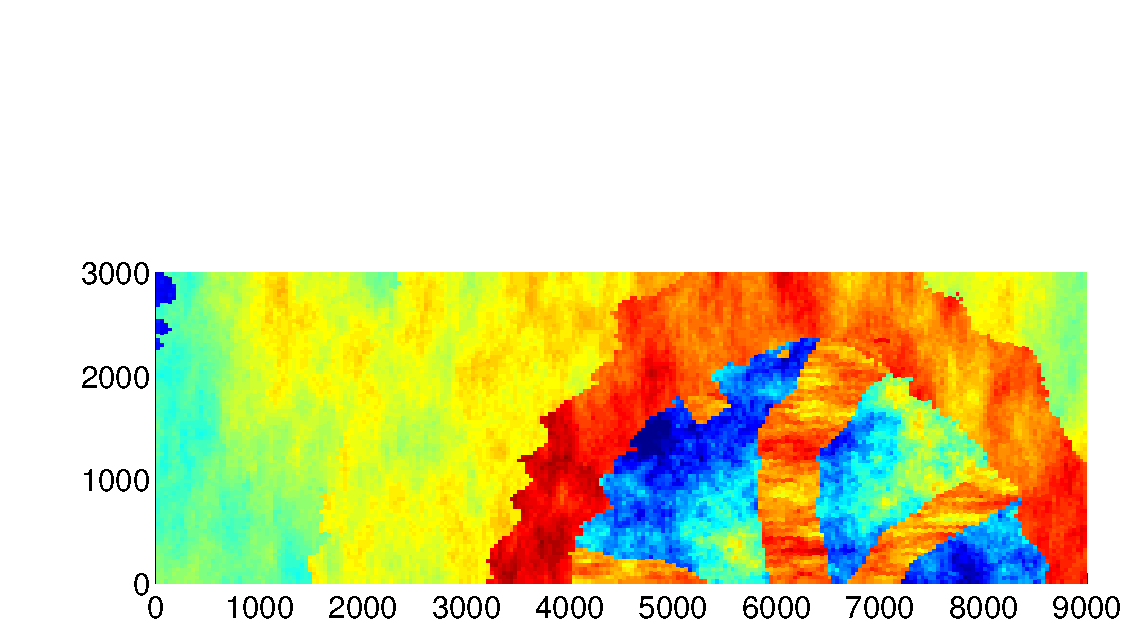
\includegraphics[trim=0.5cm 0cm 0cm 2.5cm, clip=true,width=0.5 \linewidth]
{./figurer/fineSat1}&
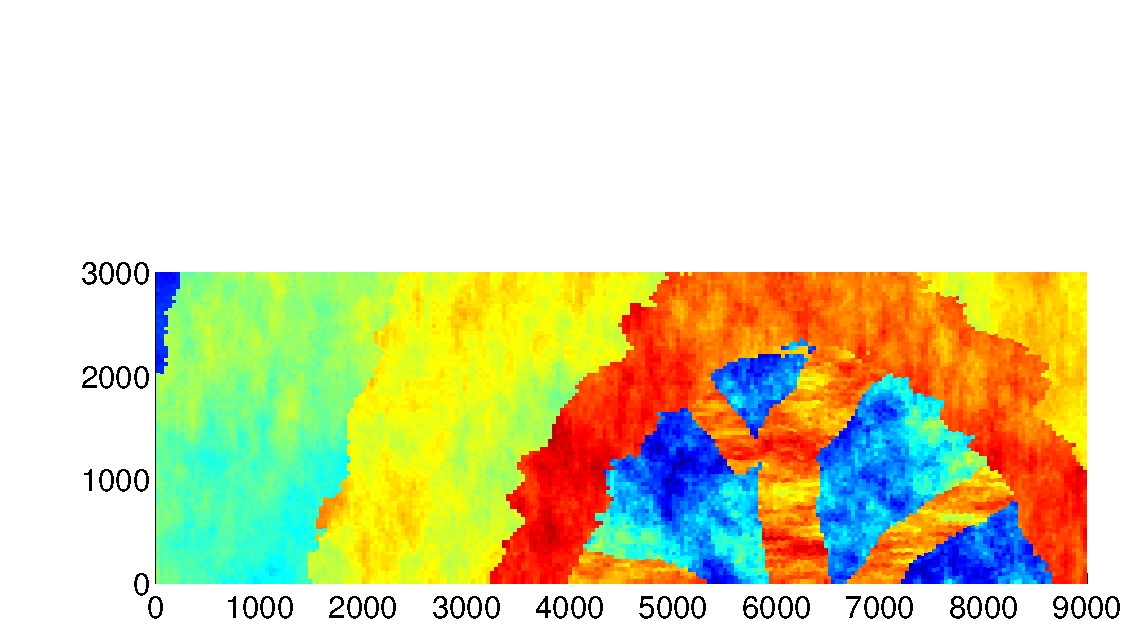
\includegraphics[trim=0.5cm 0cm 0cm 2.5cm, clip=true,width=0.5 \linewidth]
{./figurer/fineSat2}\\
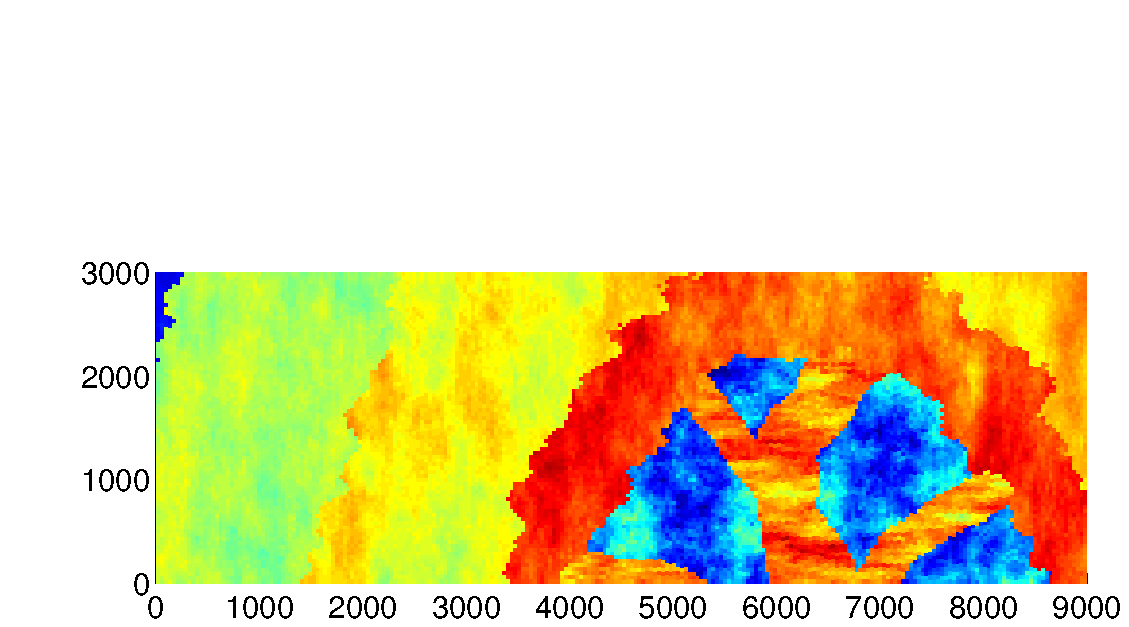
\includegraphics[trim=0.5cm 0cm 0cm 2.5cm, clip=true,width=0.5 \linewidth]
{./figurer/fineSat3}&
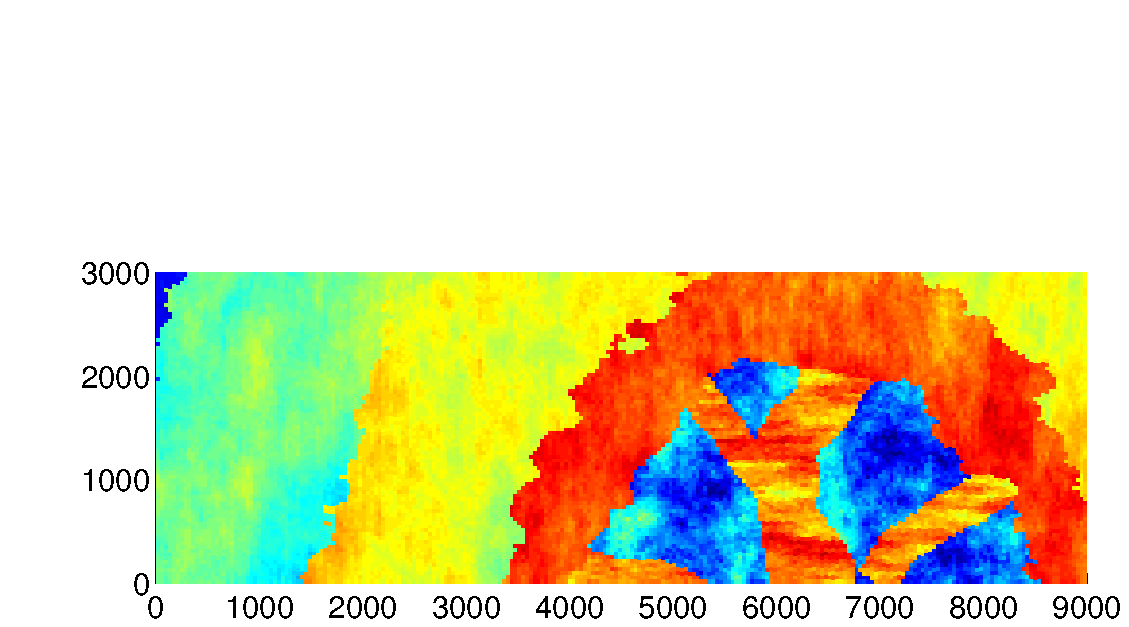
\includegraphics[trim=0.5cm 0cm 0cm 2.5cm, clip=true,width=0.5 \linewidth]
{./figurer/fineSat4}
\end{tabular}
\end{minipage}\\(b) Fine grid.
\end{tabular}
\caption{Logarithmic of lateral transmissibility plotted for four layers in fine grid versus their representative layer in the coarse grid. Plots are top view and units are cP$.$m$^3$/day/bar.}
\label{fig:upsat}
\end{figure}

Structural aspects are modeled via fault modeling. Within the SAIGIP setup, faults are considered in different levels of intensity, orientation, and transmissibility. The orientations may vary in both lateral directions, and we consider a grid that contains faults in both directions (Figure \ref{fig:fltGrd}).

\begin{figure}
\centering
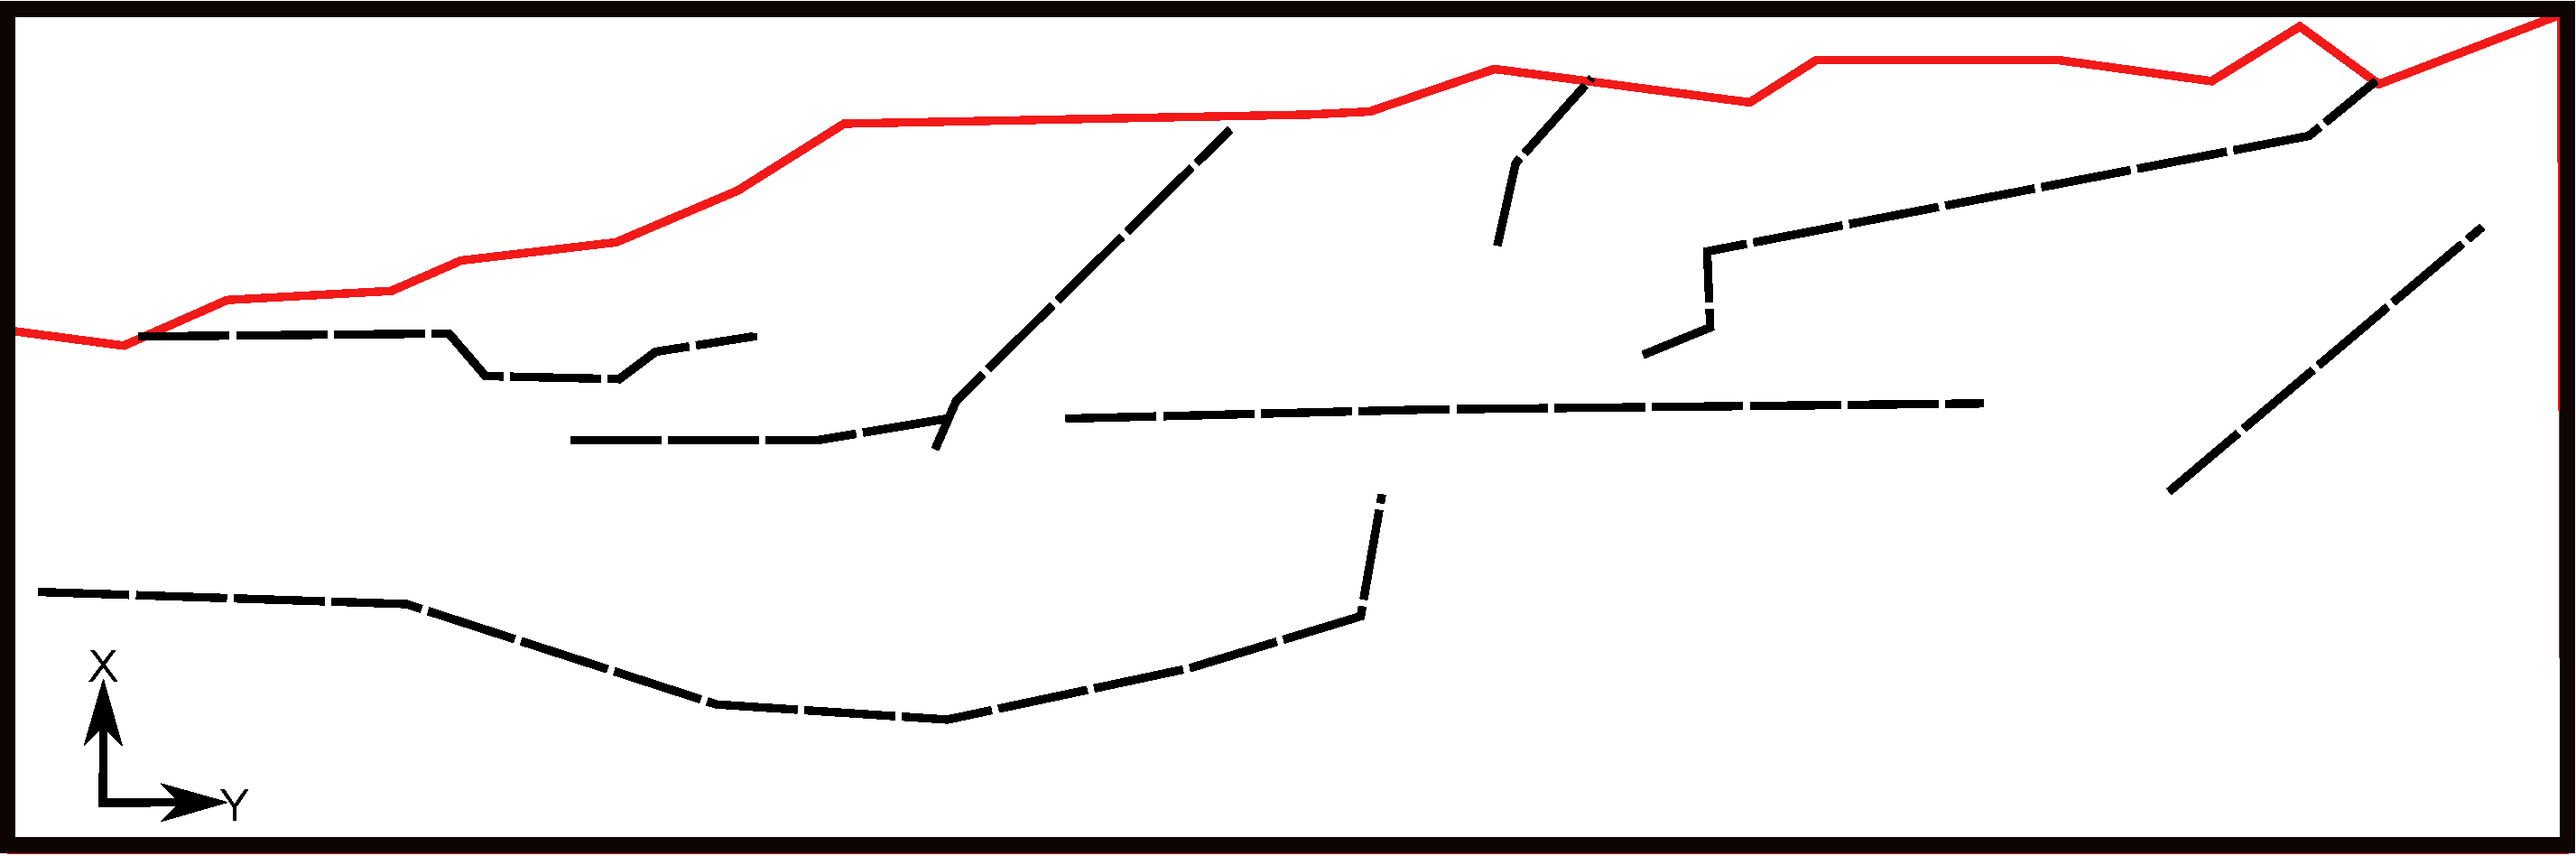
\includegraphics[width=0.8\textwidth]{./figurer/faultedGrid}
\caption{Top view illustration of faults used in the faulted grids. The fault plotted in red corresponds to the upper boundary of the model on the crest.}
\label{fig:fltGrd}
\end{figure}
%%%
Although these models were designed to study the impact of geological
heterogeneity on oil recovery, they may also be used to model a scenario in
which $\mbox{CO}_2$ is injected into an abandoned reservoir. Therefore, we have
selected five parameters from the setup and varied these parameters by combining
different levels for our $\mbox{CO}_2$ storage study. These features are
lobosity, barriers, aggradation angle, progradation, and fault. In the
following, we describe each feature briefly.


\textbf{\textit{Lobosity}}: Lobosity is a metric for describing the interplay
between fluvial and wave processes in a shallow-marine depositional system. As
the river enters the mouth of the sea, the shore-line shapes where the river
flux crashes with the waves from sea. The balance between the sediment supply from
rivers and the available accommodation space in the shallow sea defines the
shore-line shape. Sea waves smear out the shore-line, while fluvial flux from
river makes branches into the sea. Less wave effect produces more pronounced
lobe shapes around the river entrance into the sea. 

The channels made into the sea mouth by fluvial supplies contain good quality
rocks with relatively higher porosity and permeability and poor quality rock
types are located between the conductive branches. Reservoir quality decreases
with distance from the shore-face. Lobosity variation can influence the CO$_2$
injection operation and plume distribution in the aquifer. In this study, models
of three levels of lobosity are used: flat shoreline, one lobe and two lobes,
see Fig.~\ref{fig:lobCauses}.

 
\begin{figure}[tbp]%
  
  \subfloat[Lob1.]{\label{fig:lob1}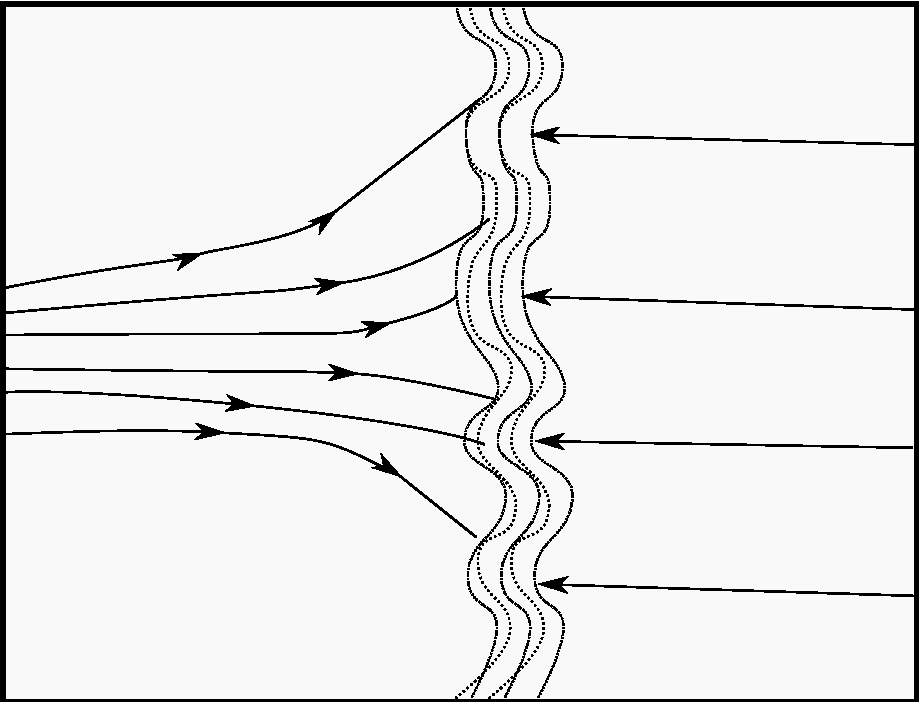
\includegraphics[width= 0.3
\linewidth]{./figurer/lob_1}} \hspace{0.5cm}
  \subfloat[Lob2.]{\label{fig:lob2}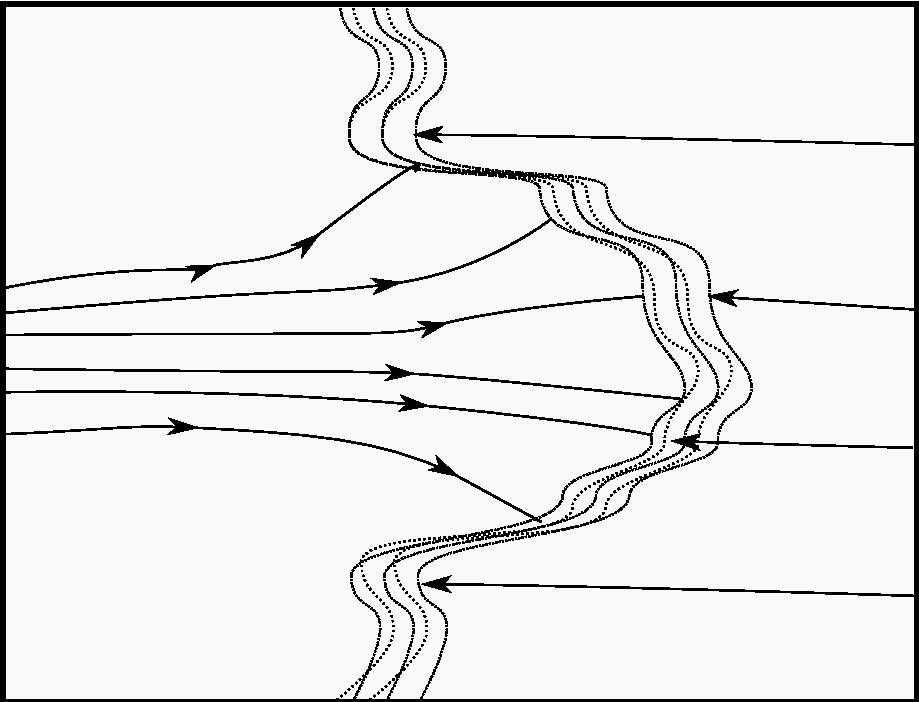
\includegraphics[width= 0.3
\linewidth]{./figurer/lob_2}}\hspace{0.5cm}
  \subfloat[Lob3.]{\label{fig:lob3}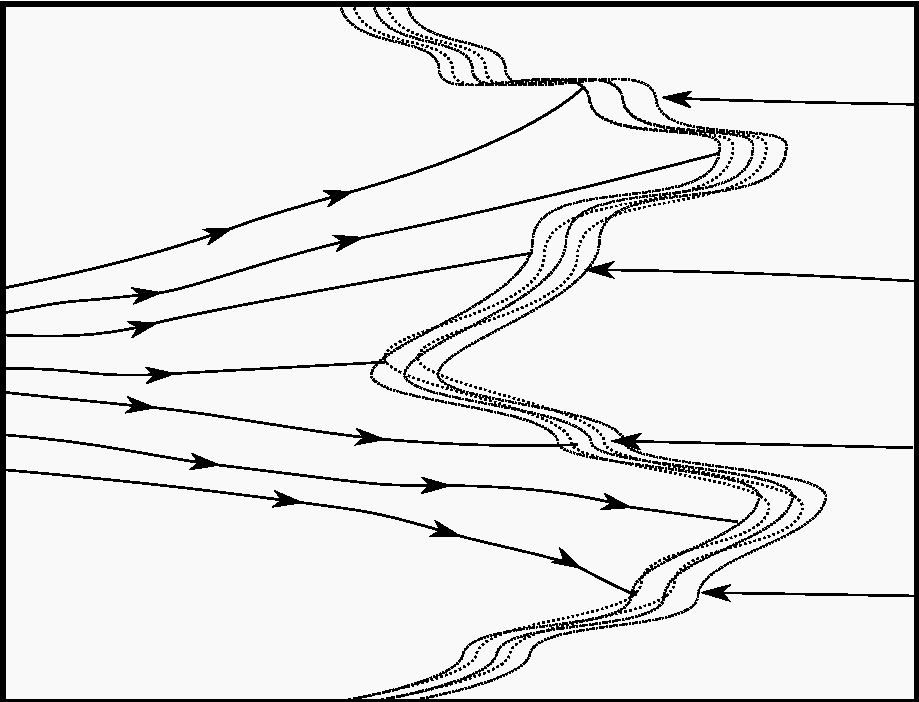
\includegraphics[width= 0.3
\linewidth]{./figurer/lob_3}}

  \caption{Lobosity levels are defined based on the shoreline shape, which is
caused by the interplay between fluvial and wave forces.}
 \label{fig:lobCauses}
\end{figure}

\textbf{\textit{Barriers}}: 
Barriers are mud-draped surfaces sitting between reservoir sections that are
caused by periodic floods in a shallow-marine depositional system. Mud-drapes
extend in both vertical and lateral directions and are potential significant
barriers to
flow.  In the SAIGUP domain used here, these barriers were modeled by defining
areas between layers with zero transmissibility multipliers. This areal coverage was designed in three levels: low (10\%), medium
(50\%), and high (90\%). We use the same variations in this study, see
Fig.~\ref{fig:barriers}.


\begin{figure}[thb]
  \centering
  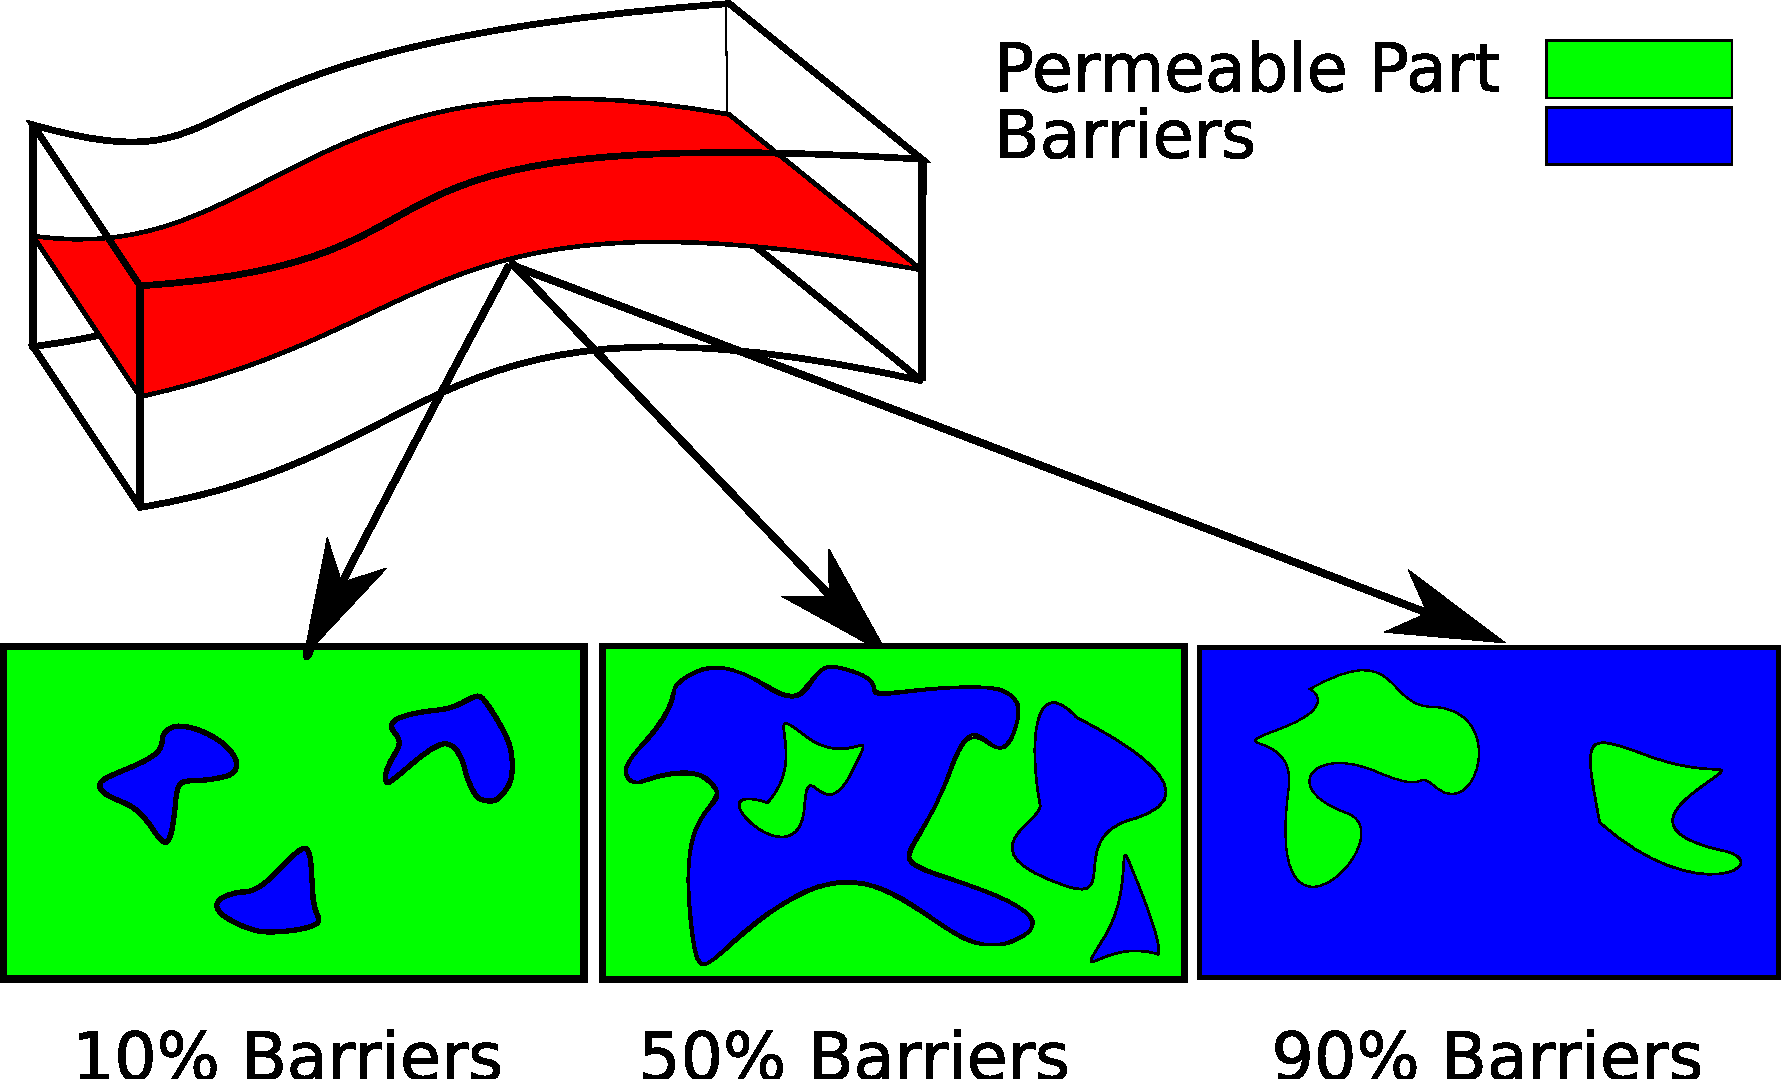
\includegraphics[width=0.65 \linewidth]{./figurer/barrier} 
  %
  \caption{Barrier levels caused by periodic floods.}
  \label{fig:barriers}
%
\end{figure}

\textbf{\textit{Aggradation angle}}:
In shallow-marine systems, the sediment supply from rivers deposits in a
spectrum of large size grains in the land side toward fine grains deep in the
basin. Amount of deposition supplied by the river compared to the accommodation
space that the sea provides defines the transition of different rock-types
between the river and the sea. If the river flux or sea level
fluctuates, the equilibrium changes into a new bedding shape based on the
balance of these
factors.

\begin{figure}[thb]
  \centering
  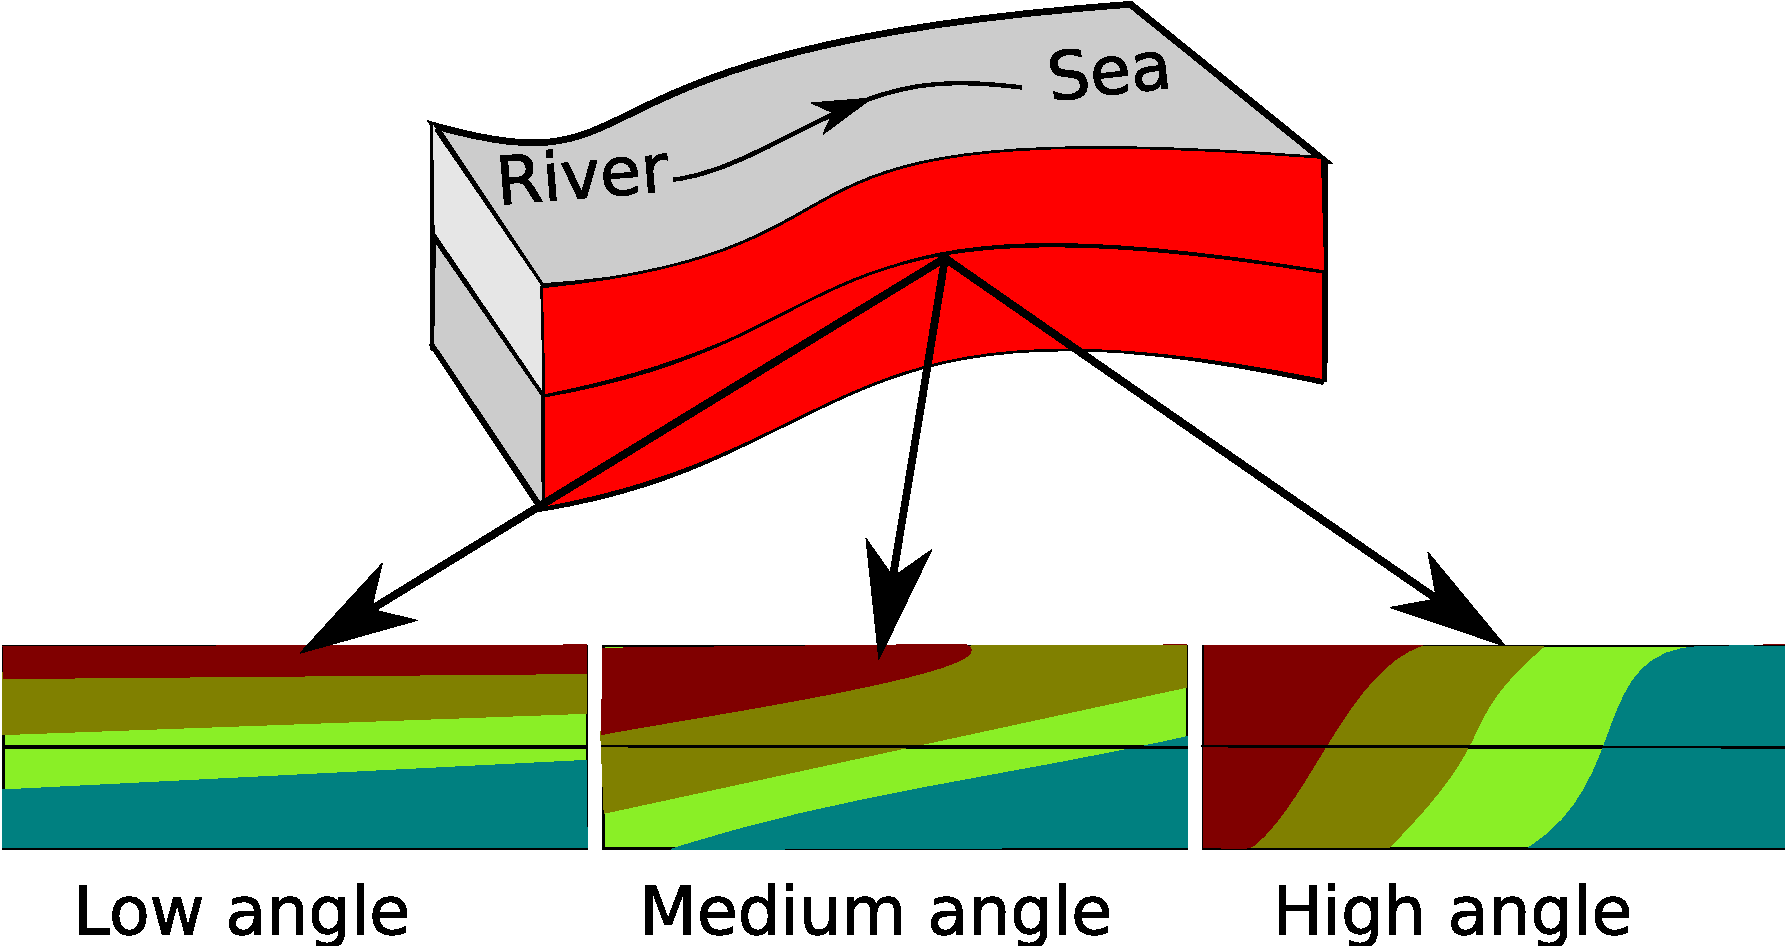
\includegraphics[width=0.65 \linewidth]{./figurer/agr} 
  %
  \caption{Aggradation angle levels.}
  \label{fig:agrLvl}
%
\end{figure}

When the river flux increases, it shifts the whole depositional system into the
sea causing an  angle between transitional deposits that are stacked on
eachother because of this shifting. This angle is called aggradation angle.
Three levels of aggradation are modeled here: low, medium and
high (Fig.~\ref{fig:agrLvl}). As we will see later, aggradation can have a major
role in influencing the $\mbox{CO}_2$ flow direction in the medium. 

\textbf{\textit{Progradation}}: 
Progradation is the depositional-dip direction between the see and the river.
Two types are considered here: up and down the dominant structural dip.
Progradation combined with lobosity can influence the plume development in the
medium, as the injected $\mbox{CO}_2$ plume migrates upward to the crest goes
through heterogeneities (Fig.~\ref{fig:proLvl}).


\begin{figure}[thb]
  \centering
  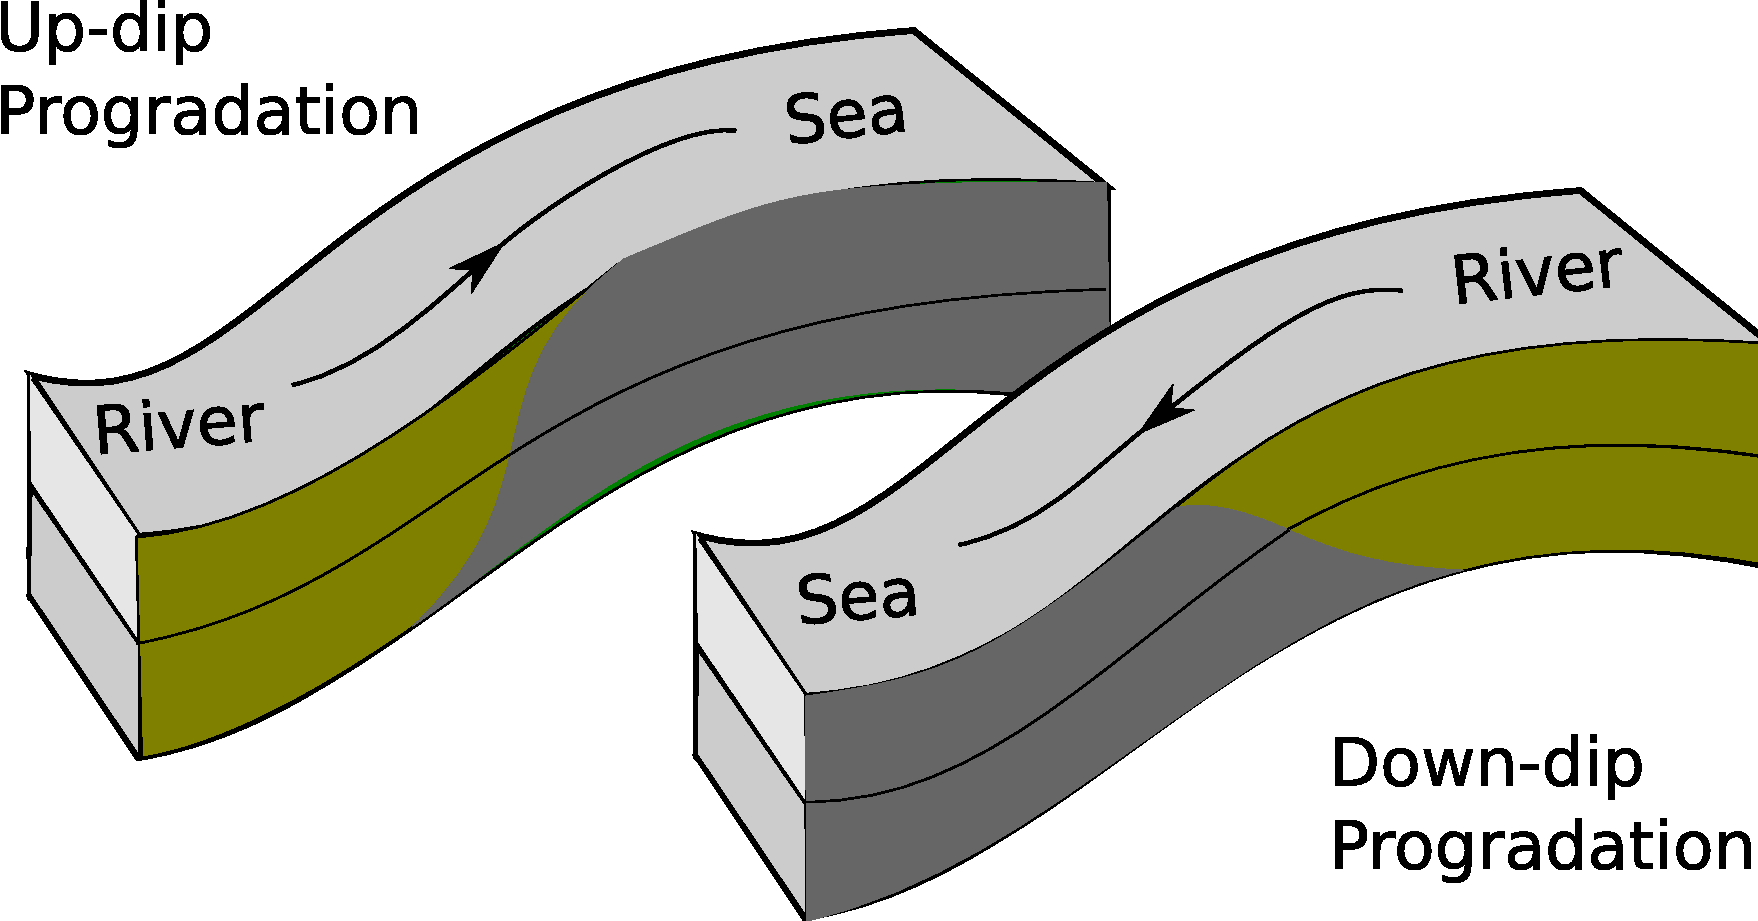
\includegraphics[width=0.65 \linewidth]{./figurer/progradation} 
  %
  \caption{Progradation levels.}
  \label{fig:proLvl}
%
\end{figure}

\vspace{1cm}
For more information about the geological modeling, see the special issue of the Petroleum Geosciences that is devoted to the SAIGUP study \cite{matthews2008assessing}. One selected realization of the SAIGUP models is available for download \cite{saigupModel} and this model is used as an example in MATLAB Reservoir Simulation Toolbox (MRST) \cite{mrstSaigup}. 

\section{Flow equations}
\label{sec:FlowEquations}
After introducing the parameters that make our geological model, we need to
define the flow problem. In this section we discuss various formulations of the governing equations describing single and two phase flow in porous medium. Solution to these type of equations is implemented in the ECLIPSE black-oil simulator that we use to model the flow. We introduce the functionalities and axillary equations required to close the flow equation system. This section also includes a brief mathematical discussion on the flow equations. We discuss various flow regimes in the medium in the next section.

\subsection{Single phase flow}

Assume a porous domain $\Omega$ with boundary $\Gamma$ as shown in Figure
\ref{fig:prsDmn}. We write the continuity equation in general form for a single
phase flowing in the domain:

\begin{equation}
  \mbox{Accumulation}+\mbox{In-Out Flux} = \mbox{Source/Sink}
  \label{eq:ak}
\end{equation}

\begin{equation}
  \int_{\Omega}\frac{\partial}{\partial t}(\phi\rho)d\tau+\int_{\Gamma}(\rho v
\cdot n)d\sigma=\int_{\Omega}qd\tau
  \label{eq:main_o}
\end{equation}
% \begin{tabular}{cc}

In Equation \ref{eq:main_o}, $\phi$ is the rock porosity, $\rho$ is the fluid
density, $v$ is the flow velocity, and $n$ is the normal vector to the boundary.
The term $q$ denotes the mass source or sink in the system. Integrations are
taken over arbitrary domain $\Omega$ with boundary $\Gamma$ (Figure
\ref{fig:prsDmn}). Flow velocity is considered at the representative elementary
volume (REV) scale for porous media \cite{bear1988dynamics}.

The resistance of a porous medium against flow results in a velocity that can be
calculated from pressure and gravity gradient and fluid properties in the
medium.
This is governed by Darcy's law for single phase flow:
 
\begin{equation}
  v=-\frac{K}{\mu}\cdot (\nabla{P}+\nabla{D}).
  \label{eq:darcy}
\end{equation} In Equation \ref{eq:darcy}, $K$ is the permeability of the
medium.
Permeability is a function of pore size distribution and connectivity and in the
macro scale, it is a measure of medium conductivity when a fluid is flowing
through the medium ( Figure \ref{fig:snglK}). $D$ is the gravity term that is a
function of fluid specific gravity and elevation in vertical direction. 

\begin{figure}[thb] 
  \centering{}
  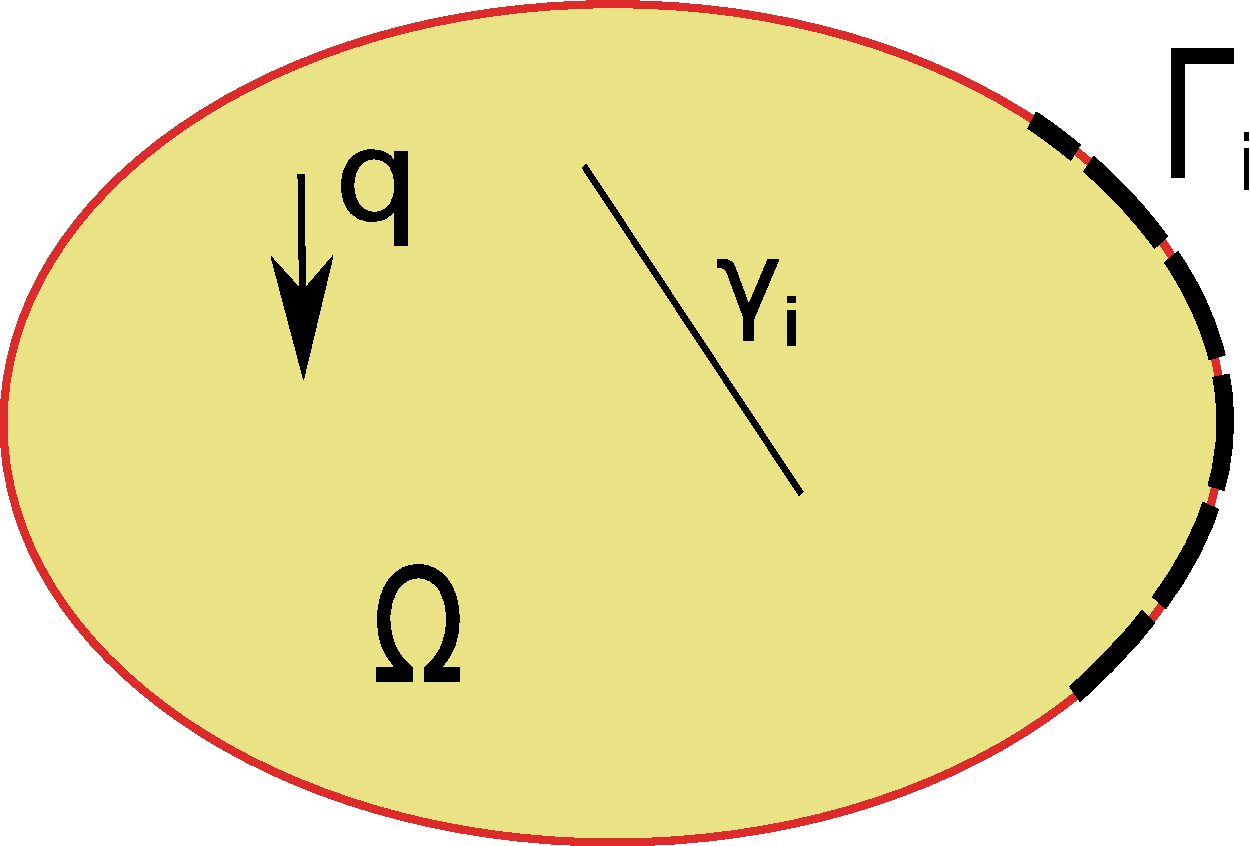
\includegraphics[scale=0.3]{./figurer/BCPB}
  \caption{Flow domain and boundaries.}
  \label{fig:prsDmn}
\end{figure}

\begin{figure}
 \centering{}
 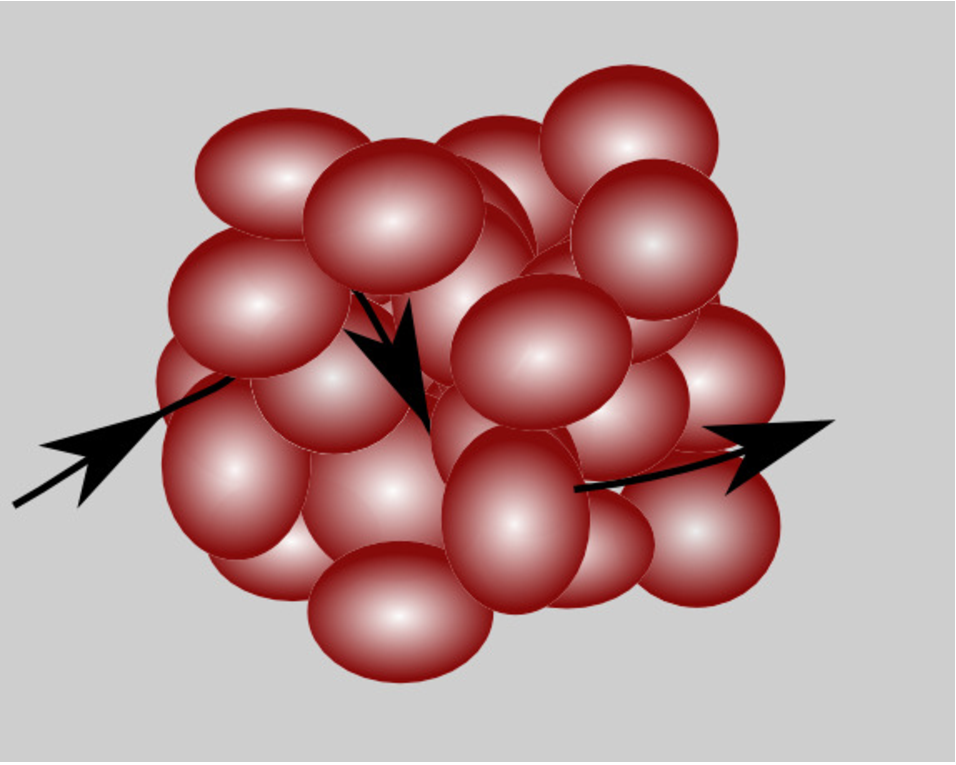
\includegraphics[width=0.35\linewidth]{./figurer/singlePerm}
 \caption{Permeability is an indication of how easy it is for the fluids to flow
trough the medium.}
 \label{fig:snglK}
\end{figure}

Substituting velocity term from Equation \ref{eq:darcy} into Equation
\ref{eq:main_o} gives:
\begin{equation}
  \int_{\Omega}\frac{\partial}{\partial t}(\phi\rho)d\tau-\int_{\Gamma}(\rho
(\frac{K}{\mu}\cdot (\nabla{P}+\nabla{D})) \cdot n)d\sigma=\int_{\Omega}qd\tau.
  \label{eq:main}
\end{equation} As a primary unknown in Equation \ref{eq:main}, the pressure depends upon the boundary conditions (as the second term left hand side of
Equation \ref{eq:main} is an integration over the boundaries of the domain). Also, any geological discontinuities in the medium
($\gamma_i$ in Figure \ref{fig:prsDmn}) appears in Equation \ref{eq:main} through the $K$ tensor and can influence pressure behavior in the domain.

The second term in Equation \ref{eq:main} can be converted into an integration
over domain $\Omega$, using divergence theorem resulting in the following:
\begin{equation}
  \int_{\Omega}[\frac{\partial}{\partial t}(\phi\rho)+\nabla \cdot (\rho
v)]d\tau=\int_{\Omega}qd\tau.
  \label{eq:div}
\end{equation} Equation \ref{eq:div} is valid for arbitrary domain $\Omega$,
hence the equality is valid for the integrands \textit{almost everywhere} in
domain $\Omega$ in the \textit{general} situation:
\begin{equation}
 \frac{\partial}{\partial t}(\phi\rho)+\nabla \cdot (\rho v)=q.
 \label{eq:diff}
\end{equation}
Fluid and rock change in volume with pressure variations. These dependencies are
defined by a parameter called total compressibility, which is approximated by a
combination of rock and fluid compressibilities:
\begin{equation}
  C_{T}\approx C_{rock}+C_{fluid},
  \label{eq:Ct}
\end{equation} where
\begin{equation}
  C_{rock}=\frac{\partial \phi}{\partial P},
  \label{eq:Cp}
\end{equation} and
\begin{equation}
  C_{fluid}=\frac{1}{\rho} \frac{\partial \rho}{\partial P}.
  \label{eq:Cf}
\end{equation} In Equation \ref{eq:Cp}, $C_{rock}$ can be assumed constant in
moderate pressure changes depicting a linear relation between pressure and
porosity. Also, Equation \ref{eq:Cf} can be expanded resulting in the following
\cite{muskatflow}:
\begin{equation}
 \rho=\rho_0 (\frac{P}{P_0})^m exp[C_{fluid}(P-P_0)].
 \label{eq:Cexp}
\end{equation} Assuming slight compression gives \cite{sahimi2011flow}:
\begin{equation}
 \rho \simeq \rho_0 + C_{fluid} \rho_0 (P-P_0).
 \label{eq:Cslg}
\end{equation}

By substituting from Equations \ref{eq:Ct}, \ref{eq:Cf}, \ref{eq:Cp}, and
Equation \ref{eq:darcy} into Equation \ref{eq:diff}, density vanishes and by
defining volumetric source/sink $\eta$, we have the single-phase diffusivity
equation:
\begin{equation}
 C_T \frac{\partial P}{\partial t}-\nabla \cdot [\frac{K}{\mu} (\nabla P -
\nabla D)] = \eta.
 \label{eq:vol}
\end{equation}

\subsection{Two-phase flow}

In a two-phase flow of $\mbox{CO}_2$ and water within porous media, interactions
between phases lead to loss of energy. This introduces specific phenomena
occurring in the pore scale that have impact on the macro scale flow
performance.
More complicated equations appear in modeling the two-phase flow compared to the
single-phase problem. First, we describe some of the conceptual two-phase
phenomena in the pore scale and then we will continue by deriving the flow
equations for two phases in the system, i.e., $\mbox{CO}_2$ and water.

\begin{figure}
 \centering{}
 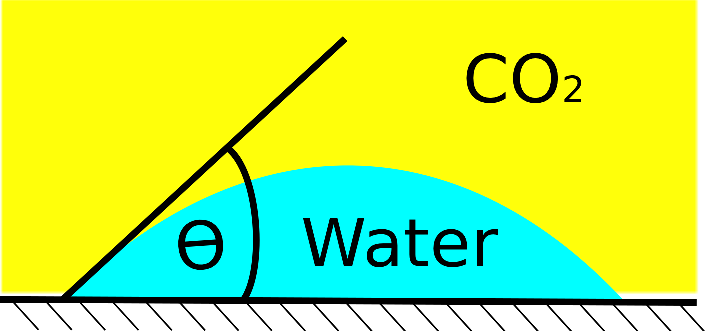
\includegraphics[width=0.35\linewidth]{./figurer/wettability}
 \caption{Wettability and interfacial tension in water-$\mbox{CO}_2$ system. Water is the wetting phase in this example.}
 \label{fig:wetting}
\end{figure}

When $\mbox{CO}_2$ and water get in contact at the pore scale, an interface
forms between them such that the energy in the system is minimized. Water and
$\mbox{CO}_2$ are also in contact with the porous medium and the interface
between them forms an angle from the solid phase in the water phase (shown by
$\theta$ in Figure \ref{fig:wetting}) that depends on their ability for
wetting the rock. This is called wettability and the phase with the
preference of wetting the solid phase is called the wetting phase. The other
phase is called the non-wetting phase.  Conventionally, $\theta$ is measured
inside the denser fluid. If $\theta < \frac{\pi}{2}$ then the denser phase is
the wetting phase. Wettability in a porous medium depends on the fluids and the
rock. It can have a significant influence in the phase displacement within the
medium. For water-$\mbox{CO}_2$ system, normally water is the wetting phase. 

\begin{figure}
 \centering{}
 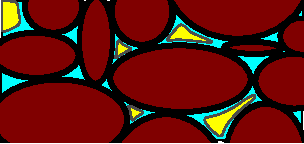
\includegraphics[width=0.35\linewidth]{./figurer/K2}
  \caption{Multi-phase flow in the pore scale.}
 \label{fig:mphf}
\end{figure}

At very low water saturations, the water phase forms molecular films surrounding the rock grains. In this situation, the water phase is immobile and can not make a continuous phase moving through the porous medium.
As water saturation in the medium increases, the layers covering the rock grains
grow in size until the saturation exceeds a critical level, above which the
water phase is able to flow in the medium. This saturation is called the
critical or connate water saturation. In a water-wet rock, once the
critical water saturation
is reached (for example, during the first deposition of sediments), it can not
go below that level by being displaced via a non-wetting phase. Therefore, when
we inject $\mbox{CO}_2$ into an aquifer, there will always be some residual
water saturation in the regions invaded by $\mbox{CO}_2$.

\begin{figure} 
  \centering{}
  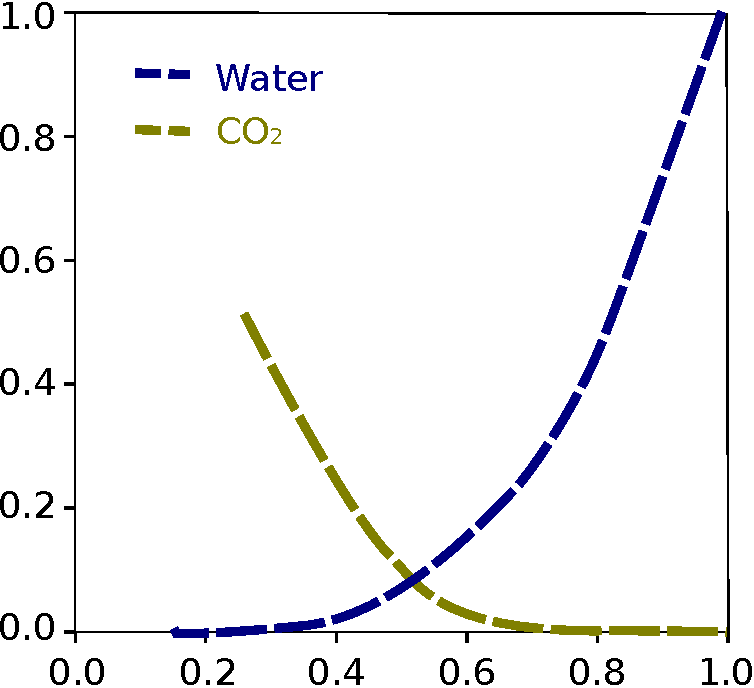
\includegraphics[width= 0.45 \linewidth]{./figurer/Kr}
  \caption{Two-phase flow and relative permeability.}
  \label{fig:kr}
\end{figure}

As a non-wetting phase, $\mbox{CO}_2$ flows in the middle part of the pore space
as shown in Figure \ref{fig:mphf}. If $\mbox{CO}_2$ saturation decreases in the
medium, it reaches a critical level under which it can not make a continuous
phase flowing through the pore-network. Tiny drops of $\mbox{CO}_2$ are trapped
in the middle of the pore space and only very large pressure difference across
the pore can move it out of the pore. This level of $\mbox{CO}_2$ saturation  is
called the residual saturation. Higher residual saturation is more interesting
for the purpose of immobilizing more volumes of injected $\mbox{CO}_2$ in the
aquifer, which reduces the risk of $\mbox{CO}_2$ leaking through any breakings
in the geological formation and channeling toward surface.

Relative ease for the phase to flow within the medium is described by
the relative
permeability parameter. Relative permeability is a function of wettability and
phase saturation. High phase saturation indicates a higher space available for
the phase to flow through that space. A sample of $\mbox{CO}_2$-water relative
permeability functions are shown in Figure \ref{fig:kr}. A library of relative
permeability curves for $\mbox{CO}_2$-water system for various rock-types is
available at \cite{krLib}.

The difference in surface tension between water and $\mbox{CO}_2$ causes a
pressure acting on the interface of the two fluids. This pressure is called
capillary pressure. In addition, capillary pressure depends on the geometry of
pores. Since the pore geometry is very irregular, it is more convenient to use
simpler geometry to derive the concept of capillary pressure. Therefore,
experimental work in the laboratory is required to specify the capillary
pressure functionality in a special case. 

Assuming a geometry of pipe to represent a pore structure, after balancing the
forces in the pore-system capillary pressure can be written in the following
form:

\begin{equation}
 P_c=\frac{2\sigma}{r}cos\theta,
 \label{eq:pcS}
\end{equation} where $\sigma$ is the interfacial tension, $\theta$ is the angle
between the interface and the solid phase, and r is the radius of the pore.

Capillary pressure is a jump in phase pressure across the interface of the two
phases. Therefore, we can relate it to the phase pressures:
\begin{equation}
 P_c=P_{nw}-P_w.
 \label{eq:pcJump}
\end{equation} Here, $P_{nw}$ is the non-wetting phase pressure and $P_w$ is the
wetting phase pressure. 


\begin{figure} 
  \centering{}
  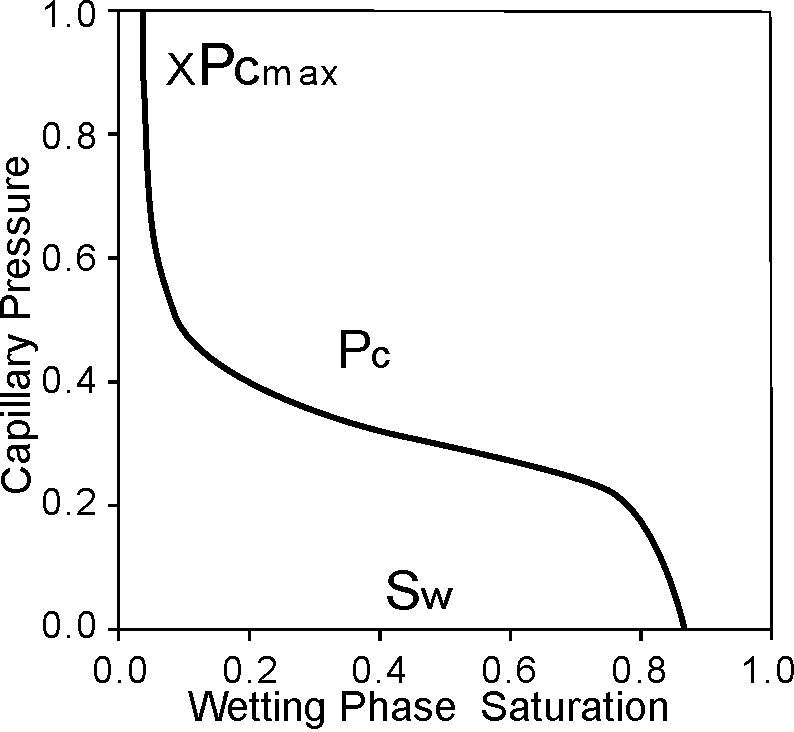
\includegraphics[width= 0.45 \linewidth]{./figurer/Pc}
  \caption{Capillary pressure can be expressed as a function of wetting
saturation. The plot is a typical curve of capillary pressure function with a
maximum of $P_{c\mbox{max}}$}
  \label{fig:pc}
\end{figure}

Capillary pressure can be expressed in an empirical relation as a function of
wetting phase saturation. Lower capillary pressure is expected for higher
wetting saturations, and capillary pressure values go up for lower wetting
saturations (Figure \ref{fig:pc}). 

Assume hydrostatic equilibrium for a porous domain in which water and
$\mbox{CO}_2$ are segregated due to buoyancy effect.  If capillary forces
are considerable in the domain, the sharp interface between water and
$\mbox{CO}_2$ in the macro scale will be replaced by a transition zone with a
spectrum of saturations between phases (Figure \ref{fig:TZ}). Due to the
hydrostatic equilibrium, phase pressure at each depth can be related to the
hydrostatic pressure of that phase:
\begin{equation}
 P_w=\rho_wgz
 \label{eq:rghw},
\end{equation}
\begin{equation}
 P_{\mbox{co}_2}=\rho_{\mbox{co}_2}gz
 \label{eq:rghc}.
\end{equation} Having the phase pressure, capillary pressure can be calculated
by
Equation  \ref{eq:pcJump}. As capillary pressure is a function of wetting
saturation, the phase saturations can be back-calculated from this functionality
and the phase saturation distribution over the medium can be found (Figure
\ref{fig:PC}):
\begin{equation}
 S_w = P_c^{-1}(S_w).
 \label{eq:pc-1}
\end{equation}



\begin{figure}
 \centering{}
 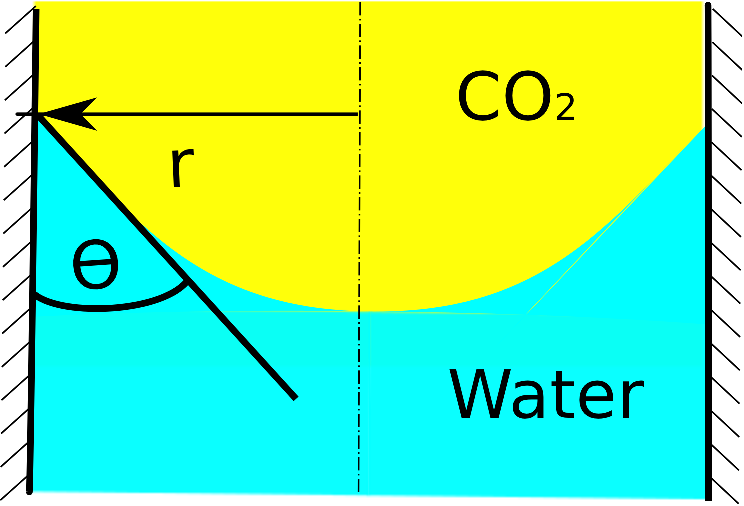
\includegraphics[width=0.35\linewidth]{./figurer/pipe}
 \caption{Capillary pressure distribution in the transition zone.}
 \label{fig:PC}
\end{figure}

\begin{figure}[thb]
 \centering{}
 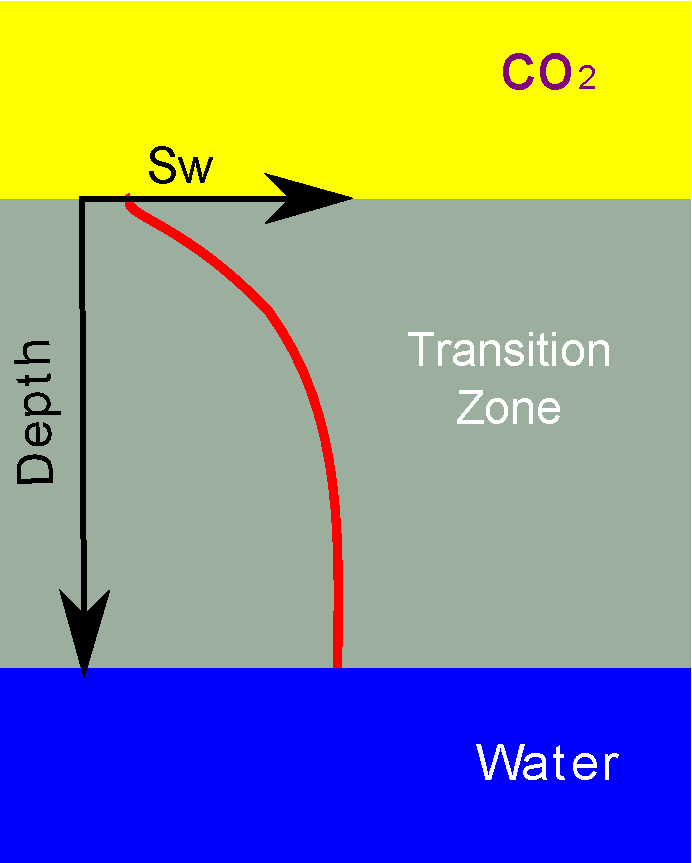
\includegraphics[width=0.35\linewidth]{./figurer/pch}
 \caption{Saturation distribution in the capillary transition zone.}
 \label{fig:TZ}
\end{figure}



We can derive mass and momentum balance for two-phase flow, similar to what we
have seen for single-phase flow. The equations must be written for each phase.
In
Equation \ref{eq:main}, the accumulation term must be considered only for one
phase mass calculated by multiplying the total accumulation mass by phase
saturation ($ S_{\alpha}$). Also the velocity is the phase velocity
$v_{\alpha}$, and the source/sink term must be written for the phase mass rate
$q_{\alpha}$.

For phase $\alpha=\{water, \mbox{CO}_2\},$ we have:
\begin{equation}
  \int_{\Omega}\frac{\partial}{\partial t}(\phi\rho_{\alpha}
S_{\alpha})d\tau+\int_{\Gamma}(\rho_{\alpha} v_{\alpha} \cdot
n)d\sigma=\int_{\Omega}qd\tau.
  \label{eq:2phs}
\end{equation} Darcy equation for two phases $\alpha=\{water, \mbox{CO}_2\}$
can be written in the following form: 
\begin{equation}
  v_{\alpha}=-\frac{K_{e\alpha}}{\mu_{\alpha}}\cdot
(\nabla{P_{\alpha}}+\nabla{D_{\alpha}}).
  \label{eq:D2phs}
\end{equation} Here, $K_{e\alpha}$ is the effective permeability for phase
$\alpha$ and can be calculated from:
\begin{equation}
 K_{e\alpha}=K_{abs}K_{r\alpha},
 \label{eq:Ke}
\end{equation} where $K_{abs}$ is the absolute rock permeability and
$K_{r\alpha}$ is the relative permeability of phase $\alpha$. $P_{\alpha}$ is
the phase pressure and $D_{\alpha}$ is the gravity term for the phase specific
gravity.



Similar to Equation \ref{eq:diff}, differential form of mass balance equation
for each of phases $\alpha=\{water,\mbox{CO}_2\}$ is as follows:
\begin{equation}
 \frac{\partial}{\partial t}(\phi\rho_{\alpha}S_{\alpha})+\nabla \cdot
(\rho_{\alpha} v_{\alpha})=q_{\alpha}.
 \label{eq:dif2p}
\end{equation}
 In this equation, $q_{\alpha}$ is the source/sink mass rate for phase $\alpha$.

 The phase saturations are related by the following equation:
\begin{equation}
  S_{water}+S_{co_2} = 1.
   \label{eq:sat}
\end{equation} Fluid properties change by pressure and temperature. Density is
mainly a function of pressure and viscosity depends upon temperature. These
functions, called by convention equation of state (EOS), must be coupled
to the system to honor fluid attribute variability
\cite{greenwood1969compressibility,duan2006equation}. 
  
Mass exchange between phases may happen leading to change in composition. That
also influences the fluid properties. In the immiscible fluids, the mass
exchange can be in small
order leading to slight changes in fluid properties. That can be modeled as a
linear function with respect to pressure and temperature. 
 
Extensive mass exchange between phases results in more nonlinear fluid property
variations that require a detailed equation of state. Also for highly miscible
fluids and high mass transfer between phases, it might be better to write mass
and momentum balance equations for components within phases in addition to phase
equations.
 
There are a number of approaches to formulate the primary unknowns in the system
of
flow equations. The direct way is to replace phase velocities from Equation
\ref{eq:D2phs} into Equation \ref{eq:dif2p}, leaving the phase pressures and
water saturation as the primary unknowns. This ends in a set of strongly coupled
equations. 
 
A popular approach for formulating the set of flow equations is the fractional
flow method \cite{binning1999practical}. In this method the total multiphase
flow problem is treated as a
single-phase flux of multi-phase mixture. Therefore, individual phases are
described as a function of total flow. This leads to separate equations for
pressure and saturation. 
 
Pressure is defined for the total flow either globally or pseudo-globally and relates to the phase pressure and saturation with auxiliary
equations. The fractional flow approach keeps the governing equations in the
form of single flow equations, and numerical schemes for single-phase flow can
be revised into efficient schemes for multi-phase problems.
 
Pressure and saturation equations have different mathematical nature: pressure
has a diffusive character of an elliptical nature, which is numerically more
stable than the saturation equation. Saturation equation is of
convection-diffusion form with hyperbolic character in the convection part. The
convection operator in saturation equation can be highly non-linear due to
strong coupling of saturation and phase velocity. This nonlinearity can lead to
shocks and discontinuities in the saturation solution.
 
As an example of fractional flow formulation, global pressure $P_t$ is defined
based on phase pressures:
 
\begin{equation}
 P_t=\frac{1}{2} (P_W+P_{CO2})-\int^{Sw}_{S_w
\mid_{P_c=0}}(f_w-\frac{1}{2}){P'}_c(S_w)dS_w,
 \label{eq:GP}
\end{equation} where water fractional flow $f_w$ is defined as:
\begin{equation}
 f_w(S_w)=\frac{\frac{K_{rw}}{\mu_w}}{\frac{K_{rw}}{\mu_co_2}+\frac{K_{rco_2}}{
\mu_co_2}}.
 \label{eq:fw}
\end{equation} The total velocity is defined as:
\begin{equation}
 v_t=v_w+v_{co_2}.
 \label{eq:VT}
\end{equation}If capillary and gravity effects are negligible, saturation
equation can be solved analytically, e.g. via Buckley-Leverett technique, or
method of characteristics.


\section{Flow regimes}
\label{sec:FlowRegimes}

A major part of our studies includes modeling physical phenomena occurring
within
flow through porous media. Various phenomena occurs during a complete sequence
of $\mbox{CO}_2$ sequestration. During injection the forces imposed by the injector
dominate the flow behavior in a region around the injector. When $\mbox{CO}_2$
plumes develop in a thin layer moving along the stratigraphical structure, a
large interface between water and $\mbox{CO}_2$ enhances the diffusion phenomena
and lets more $\mbox{CO}_2$ be dissolved into water. Convection of water with
dissolved $\mbox{CO}_2$ leads to complicated flow regimes.

The injected $\mbox{CO}_2$ undergoes various stages until it is stored
underground. We consider two stages in our studies: injection, early
migration, and long-term migration. Many forces act on flow within medium, each
of which requires a set of modeling parameters. Simplifying assumptions for flow
modeling can be justified at each stage with relevance to the dominating forces in
the medium.

The following can be recognized as forces acting on the medium at the scale at
which Darcy velocity is defined:

\begin{itemize}
\item Forces due to pressure gradients, mostly imposed by injectors (and/or
producing wells).
\item Buoyancy due to density contrasts between flowing phases. Gravity acts in the vertical direction.
\item Capillary forces due to inter-facial tensions.
\item Hysteresis due to sequencing of imbibition and drainage during flow in
the porous medium.
\item Convection forces due to gradients of density within one phase.
\item Diffusion due to concentration gradients of one component.
\item Reaction due to chemical reactions between phases and rock.
\end{itemize}

Modeling all forces acting on a porous medium is not practical, and we need to look at each flow regime separately by neglecting some forces that have a minor role. Herein, we discuss the main forces during injection and within long term migration.


\subsection{Injection and early migration}

Injection of $\mbox{CO}_2$ in the underground happens by forcing $\mbox{CO}_2$
mass through an injector into the medium. This poses a pressure gradient around the injector causing flow within the near bore region. Some authors call the force due to pressure difference `viscous force', since viscosity has an important role in transferring the stress due to pressure difference in the porous medium resulting in fluid mobility. We use the same term throughout this thesis. 

Viscous and gravity forces are the two major forces acting on the region around the injector during injection. Depending on fluid properties and distance from injection point, force balance changes. Gravity causes rapid phase
separation resulting in upward movement of $\mbox{CO}_2$. Gravity forces
dominate two-phase regions far from the injector with lower viscous flow velocity compared to near well locations, where the flow velocity is high. At each position in the medium, a force balance results in a total force vector that may cause flow in a particular direction ( Figure \ref{fig:injF}).

Attempts in the literature on evaluating force interplay during a multiphase
flow regime incorporating injection in the porous medium, employ sensitivity
analysis on flow attributes such as flow velocity and pressure. There a number of publications that discusses reducing a complicated flow problem into a simplified problem by taking plausible assumptions \cite{fayers1959effect,dong1999effect,nordbotten2005injection,
yortsos1983analytical,rapoport1953properties,farajzadeh2011analytical,
yang1992analytical,chen1990integral,bentsen1993effect}. Utilizing analytical
solutions gives the flexibility of examining a wide range of parameter
variations within the model, enjoying a fast evaluation of the
corresponding flow behavior. Semi-analytical and numerical sensitivity analysis
are also practiced in the literature to involve more physical modeling
features in the flow performance
evaluations\cite{rosado2007analysis,allen1986theoretical,alkan2010impact}.


The flow equations can be normalized to a dimensionless version that is used in
many studies discussing the capillary and gravity influence on the flow.
Herein, we give the method reported in \cite{fayers1959effect}. If we assume incompressible flow in a one-dimensional domain $\Omega$
without any source/sink, Equation \ref{eq:dif2p} reduces to the following for
the wetting phase:

 \begin{equation}
  \phi \frac{\partial s_{w}}{\partial t}+ \frac {\partial v_w} {\partial x}=0,
  \label{eq:2p1d}
 \end{equation} and Darcy equation for one
dimension
flow becomes:
 \begin{equation}
  v_w=-K\frac{k_{rw}}{\mu_w}(\frac{\partial P_w}{\partial t} + \rho_w g z).
  \label{eq:D1d}
 \end{equation} Here, $z$ is the elevation and $g$ is the gravitational
acceleration. The system is closed by Equations \ref{eq:sat} and \ref{eq:pcJump}
. We can define the dimensionless variables as follows:
 \begin{equation}
  X^*=\frac{x}{L};~T^*=\frac{tv_t}{L\phi};~\mbox{ and }P^*_c=\frac{p_c}{\pi_c},
  \label{eq:var*}
 \end{equation} where $L$ is a length constant in the problem and $\pi_c$ is a
capillary pressure normalizing constant. After reformulating Equation
\ref{eq:2p1d}, fractional flow can be written in the following form:
 \begin{equation}
  f_w=G(S_w)+C(S_w)\frac{\partial S_w}{\partial X^*},
 \end{equation} where $S_w$ is the normalized wetting phase saturation, $G$ is
the gravity contribution, and $C$ is the capillary contribution to
the flow. The gravity and capillary contributions, $G$ and $C$, are expressed
by quantities relative to the viscous force \cite{hadley1956theoretical} and we
have:
 \begin{equation}
  G(S_w)=F_w(1-N_Gk_{rnw}),
  \label{eq:GrCont}
 \end{equation}
 \begin{equation}
  C(S_w)=N_{nw}F_wk_{rnw}\frac{dP_{c}}{dS_w},
  \label{eq:PcCont}
 \end{equation} wherein: 
 \begin{equation}
  F_w=(1+\frac{k_{rnw}}{\mu_{nw}}\frac{\mu_w}{k_{rw}})^{-1},
  \label{eq:Fn}
 \end{equation}
 \begin{equation}
  N_c=\frac{k\pi_c}{\mu_{nw}Lv_t},
  \label{eq:Nc}
 \end{equation}
 \begin{equation}
  N_G=(k\frac{k(\rho_w-\rho_{nw})gz}{\mu_{nw}v_t}).
  \label{eq:Fn}
 \end{equation} Having these definitions, Equation \ref{eq:2p1d} reshapes into:
 \begin{equation}
  \frac{\partial S_w}{\partial T^*}+\frac{dG(S_w)}{dS_w}\frac{\partial
S_w}{\partial X^*}+\frac{\partial}{\partial X^*}\left( C(S_w)\frac{\partial
S_w}{\partial X^*}\right)=0.
  \label{eq:2p1dN}
 \end{equation} Applying specific type of capillary pressure and relative
permeability function may lead to simplified forms of Equation \ref{eq:2p1dN}
with the possibility of having an analytical
solution \cite{yortsos1983analytical}. 

Some important conclusions in the literature from sensitivity studies on
capillary, gravity and viscous forces are summarized here and inferred for
$\mbox{CO}_2$ injection application:

\begin{itemize}
 \item Gravity and capillary pressure will only influence the flow speed
significantly for slow displacement rates. Therefore, around the injection point where normally fluids are flowing with a relatively high speed, viscous forces are dominant.
 
 \item If capillary is of any significance, ignoring capillary forces in
modeling the injection of $\mbox{CO}_2$ results in a pessimistic $\mbox{CO}_2$
sweep efficiency. Capillary helps in the spreading of $\mbox{CO}_2$ in the
frontal $\mbox{CO}_2$-water interface.
 
 \item Less capillary forces in the porous medium allows more space for
$\mbox{CO}_2$. This enhances the density segregation due to gravity forces.
\end{itemize}

The main focus in the series of work in this thesis has been to assess the flow
influence by heterogeneity during injection time and early $\mbox{CO}_2$
migration. For $\mbox{CO}_2$ injection problems, one objective is to maximize
the rate of injection and aligned with that we use relatively high injection
rates in our studies. Therefore, we did not include capillarity forces for
modeling the high displacement rates within heterogeneities, which can be
justified by the results in the literature.


\begin{table}[tbf]
  \center
  \caption{Spatial scales for $\mbox{CO}_2$ storage. Ranges are extracted from
  \cite{celia2011geological}.}
  \begin{tabular}{ |l|| l| }
    \hline
    Feature& Spatial scale \\
    \hline
    Capillary fringe & 10cm-->10m\\
    \hline
    Plume radius & 10km-->100km\\
    \hline
    Pressure perturbation & 50km-->500km\\
    \hline
    Migration distance & 50km-->500+km\\
    \hline
  \end{tabular}
  \label{tab:xscl}
\end{table}

\begin{table}
\center
  \caption{Temporal scales for $\mbox{CO}_2$ storage. Ranges are extracted from
\cite{celia2011geological,gunter1997aquifer}.}
\begin{tabular}{ |l|| l| }
    \hline
    Feature& Temporal scale \\
    \hline
    Density segregation & 1 month-->5+ years\\
    \hline
    Capillary segregation & 1 year-->50 years\\
    \hline
    Injection period & 5 years-->50 years\\
    \hline
    Convective mixing & 20 years-->1000 years\\
    \hline
    Plume migration & few hundred years-->1000 years\\
    \hline
    Mineral reaction & 500 years-->100000 years \\
    \hline
  \end{tabular}
  \label{tab:tscl}
\end{table}

\subsection{Long term migration}

The injected \coo\ volume in the geological formation will travel below
the sealing cap by buoyancy forces due to the density difference between water
and \coo. One concern is to have \coo\ stored safely, and the mobile
\coo\ is at risk of leaking through any imperfections in the sealing
layers and abandoned wells. Molecular diffusion occurs at the interface of water
and \coo\ and this mass transfer from the \coo\ plume into water
increases the water density. Transition of \coo\ from mobile phase
into water with dissolved \coo\ is helping the safe storage of
\coo: the heavier water with dissolved \coo\ has the tendency
of moving downward. Time scale for this convective mixing is of the order of
several hundreds years (Table \ref{tab:tscl}). Yet, this is not the end and   the
dissolved $\mbox{CO}_2$ can react with the porous medium ending up in a solid
phase and it can be stored permanently in a process called mineral trapping.
This is an 
extremely slow process and it can take thousands of years
\cite{gunter1997aquifer}.

Mixing of $\mbox{CO}_2$ and water in the long-term happens through phases with various time scales and physical phenomena. Diffusion of
$\mbox{CO}_2$ in water continues and layer of water with dissolved
$\mbox{CO}_2$ builds up below the $\mbox{CO}_2$ plume until it forms heavy parts convecting in
the form of unstable fingers, as shown in Figure \ref{fig:migF}.

The onset time for the convective mixing is important in terms of storage
safety. This time depends on the Rayleigh number in the medium:

\begin{equation}
 Ra = \frac{Kg\Delta \rho H}{D_c \phi \mu}.
 \label{Ra}
\end{equation} Here, $\Delta \rho$ is the density difference between the water and
$\mbox{CO}_2$ phases and $D_c$ is the diffusion coefficient of $\mbox{CO}_2$
into water phase. The higher density sitting on top of lower density makes an
unstable system and the medium must have a minimum Rayleigh number to
have a growing instability for a small perturbation in the medium.
Heterogeneities in the medium can initiate perturbations, reducing the
instability onset time \cite{hassanzadeh2005modelling,elenius2012time}.
Therefore, heterogeneity is an important factor that must be considered when we
are choosing an aquifer for $\mbox{CO}_2$ storage.

Capillary fringe in the plume can enhance the onset of the convective mixing. It can
speed up the process up to five times \cite{eleniuseffects}.

The flow equations for convective mixing are a set of mass and momentum balance
for component $c=\{\mbox{Water},\mbox{CO}_2\}$ within phase
$\alpha=\{\mbox{Wetting},\mbox{Non-Wetting}\}$:
\begin{equation}
\frac{\partial}{\partial t} \underset{\alpha}{\sum}\phi S_\alpha \rho_\alpha
X_{\alpha}^c + \nabla \cdot \underset{\alpha}{\sum} \rho_\alpha X_{\alpha}^c
v_\alpha = 0,   
%  \phi\frac{\partial c}{\partial t}+ \left[\nabla c v_c -D_c \nabla c \right],
 \label{eq:massCo2}
\end{equation} and 
\begin{equation}
 v_\alpha = -\frac{k_{r_\alpha}K}{\mu_\alpha} \left[  \nabla
P_\alpha-\rho_\alpha g z \right]
 \label{eq:darcyCo2}
\end{equation} where $X_{\alpha}^c$ is the mole fraction of
component $\mbox{c}$ in phase $\alpha$ \cite{elenius2010co2}. 

\begin{figure}[tbp!]%
  \hspace{0.2cm}
  \subfloat
  [Injection and early migration flow
regime.]{\label{fig:injF}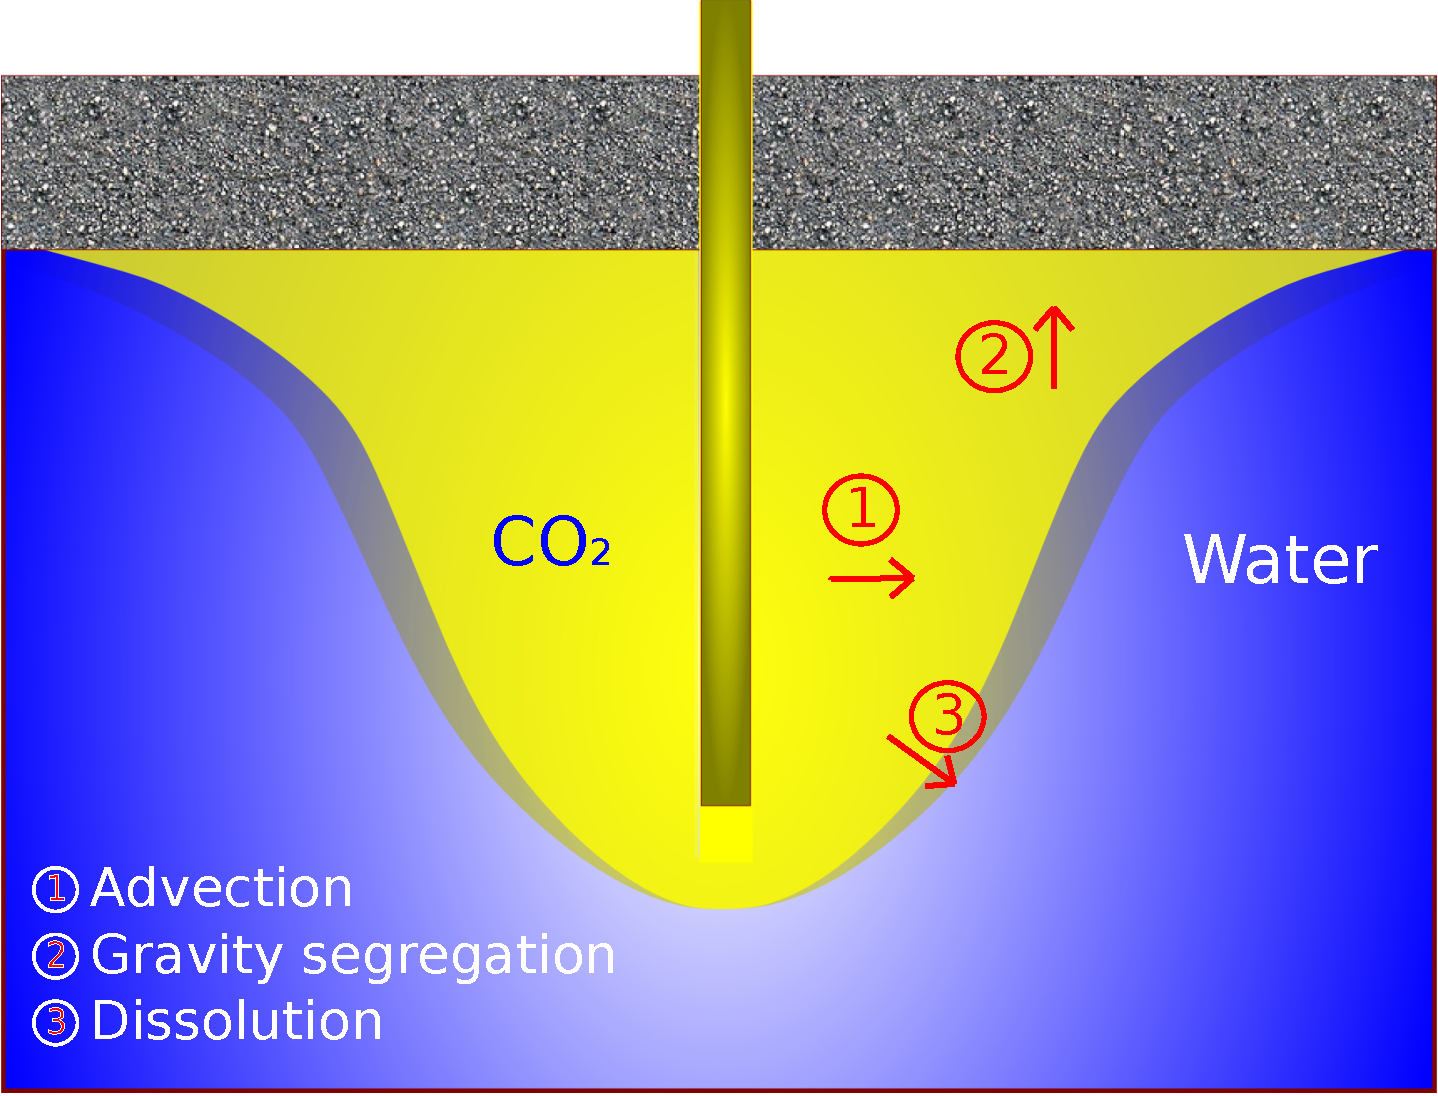
\includegraphics[width= 0.41
\linewidth]{./figurer/forceBalance_injection}} 
  \hspace{0.1cm}
  \subfloat
  [Long-term migration flow regime.]{\label{fig:migF}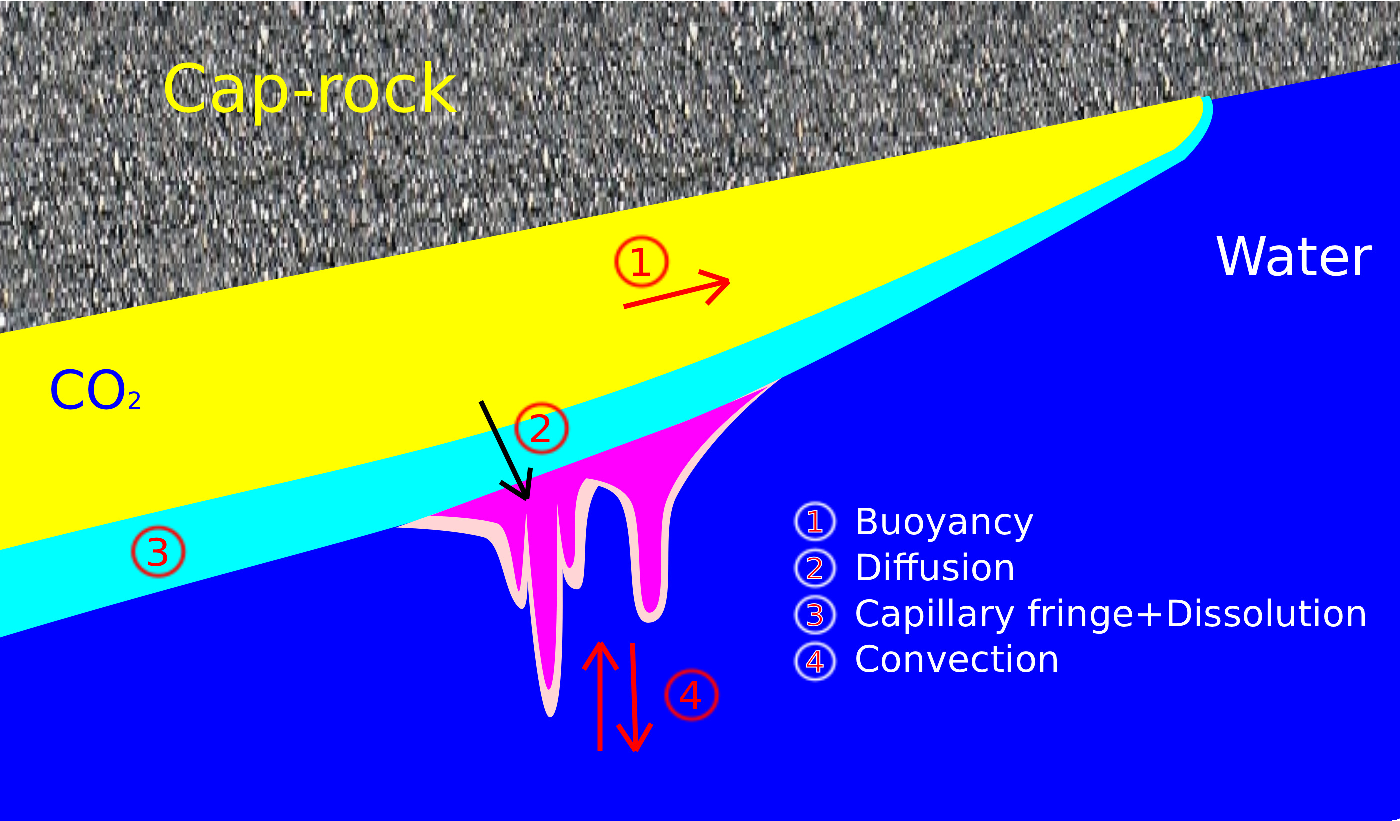
\includegraphics[width= 0.5
\linewidth]{./figurer/forceBalance_longMigration}}
  \caption{Flow regimes in geological $\mbox{CO}_2$ storage.}
 \label{fig:Frc}
\end{figure}


\section{Vertical averaging}

In this section we discuss the common approach used in modeling the migration
of $\mbox{CO}_2$ in large scale aquifers. This is a specific type of multi-scale
modeling, at which we work with two models with two and three
dimensions. A $2\mbox{D}$ model is extracted from the corresponding $3\mbox{D}$ 
model to reduce the computation costs and in some cases the accuracy can be
enhanced by reducing the numerical diffusion as we will discuss here.

Spatial gradients of flux and pressure appear in the the flow equations can be
decomposed into lateral and vertical components. For a three dimensional
problem with the set of unit vectors
$\{\overrightarrow{i},\overrightarrow{j},\overrightarrow{k}\}$, the gradient
operator can be written as the following:
\begin{equation}
    \nabla = \nabla_{\ell} + \nabla_{\\v},
    \label{eq:grd}
\end{equation} where:
\begin{equation}
    \nabla = \frac{\partial}{\partial x}\overrightarrow{i} +
\frac{\partial}{\partial y}\overrightarrow{j} +
\frac{\partial}{\partial z}\overrightarrow{k},
    \label{eq:grdc}
\end{equation}
\begin{equation}
    \nabla_{\ell} = \frac{\partial}{\partial x}\overrightarrow{i} +
\frac{\partial}{\partial y}\overrightarrow{j},
    \label{eq:grdpllc}
\end{equation}
\begin{equation}
    \nabla_{\\v} = \frac{\partial}{\partial z}\overrightarrow{k}.
    \label{eq:grdvrtc}
\end{equation} $x$, $y$, and $z$ are the location space components in the three
directions.


The geological formation tops are not necessarily oriented horizontally, but
they
are normally close to horizontal. In $\mbox{CO}_2$ storage problems the lateral
scale is
orders of magnitude larger than the vertical direction. Therefore, the
variations in the vertical direction are relatively negligible and for a
quantity of interest $\Psi$ we have:

\begin{equation}
 \int_{A}\nabla\Psi d\tau >> \int_{\varsigma}\nabla\Psi dz, 
 \label{eq:intPsi}
\end{equation} where $A$ is an arbitrary horizontal surface in the model and
$\varsigma$ is the vertical interval of the domain. Hence, with large lateral
scales we can consider average values across the vertical direction for
parameters and variables in the flow equations. This reduces the problem from
$3\mbox{D}$ to $2\mbox{D}$. In this case we need to relate the parameters in
the two dimensional and three dimensional problems. If this relation is not
extremely non-linear the flow solutions can be obtained considerably faster on
a two dimensional problem.

In a distance from the injection point, vertical equilibrium assumption is
applicable. The density difference between water and $\mbox{CO}_2$ results in a
rapid
segregation of the two phases. A layer of $\mbox{CO}_2$ sits on top of water
table and in
the presence of considerable capillary forces a capillary transition zone forms
between water and $\mbox{CO}_2$ zones (Figure \ref{fig:VC}).

The vertical equilibrium assumption facilitates the flow equation averaging
across the vertical direction $\varsigma$. The phase distribution can be
calculated from the volume calculations and capillary inverse function for the
transition zone as mentioned in \ref{sec:FlowEquations}. Phase pressure
variation versus depth follows the hydrostatic gravitational gradient for each
phase.

The two dimensional version of flow equation can be written in the following
form, assuming incompressible fluids \cite{moll2011field,celia2011geological}:

\begin{equation}
 \tilde{\phi}\frac{\partial \tilde{S}_{\alpha}}{\partial
t}-\nabla_{\ell}\cdot \tilde{v_{\alpha}}=\tilde{\eta}_{\alpha},
\label{eq:cont_}
\end{equation} which follows by two dimensional Darcy equation:

\begin{equation}
\tilde{v}_{\alpha}=-\tilde{K}\tilde{\lambda}_{\alpha}(\nabla_{\ell}
\tilde{P}_{\alpha}-\tilde{\rho}_{\alpha}\tilde{g}). 
\label{eq:Darcy_}
\end{equation}Herein, tilde sign denotes the two dimensional parameter or
variable that is the vertically averaged of corresponding parameters and
variables in the three dimensional problem. The averaging over vertical
direction care defined in the following:

\begin{equation}
\tilde{\phi}=\frac{1}{H}\int_0^H\phi dz,
\label{eq:phi_}
\end{equation}
\begin{equation}
\tilde{K}=\frac{1}{H}\int_0^H K dz,
\label{eq:K_}
\end{equation}
\begin{equation}
\tilde{\lambda_{\alpha}}=\frac{1}{H}K^{-1}\int_0^HK\lambda_{\alpha} dz.
\label{eq:lambda_}
\end{equation} Note that $\tilde\lambda_\alpha$ is a tensor, because it is
defined such that the $2\mbox{D}$ Darcy equation is consistent with the
$3\mbox{D}$ Darcy equation. The variables in the $2\mbox{D}$ equations are
defined in the following:
\begin{equation}
\tilde{v}_\alpha=\frac{1}{H}\int_0^H v_\alpha dz,
\label{eq:v_}
\end{equation}
\begin{equation}
\tilde{s}_\alpha=\frac{1}{\tilde{\phi}H}\int_0^H \phi s_\alpha dz,
\label{eq:s_}
\end{equation}
\begin{equation}
\tilde{P}_\alpha=p_{\alpha}(z_D),
\label{eq:p_}
\end{equation}
\begin{equation}
\tilde{\eta}_\alpha=\frac{1}{H}\int_0^H \eta_\alpha dz.
\label{eq:eta_}
\end{equation} The hydrostatic equilibrium results in a constant phase pressure
gradient over the vertical direction. Therefor, the phase pressure at any datum
depth $z_D$ in the medium can be used into the $2\mbox{D}$ flow equations. 


\begin{figure}[thb]
 \centering{}
 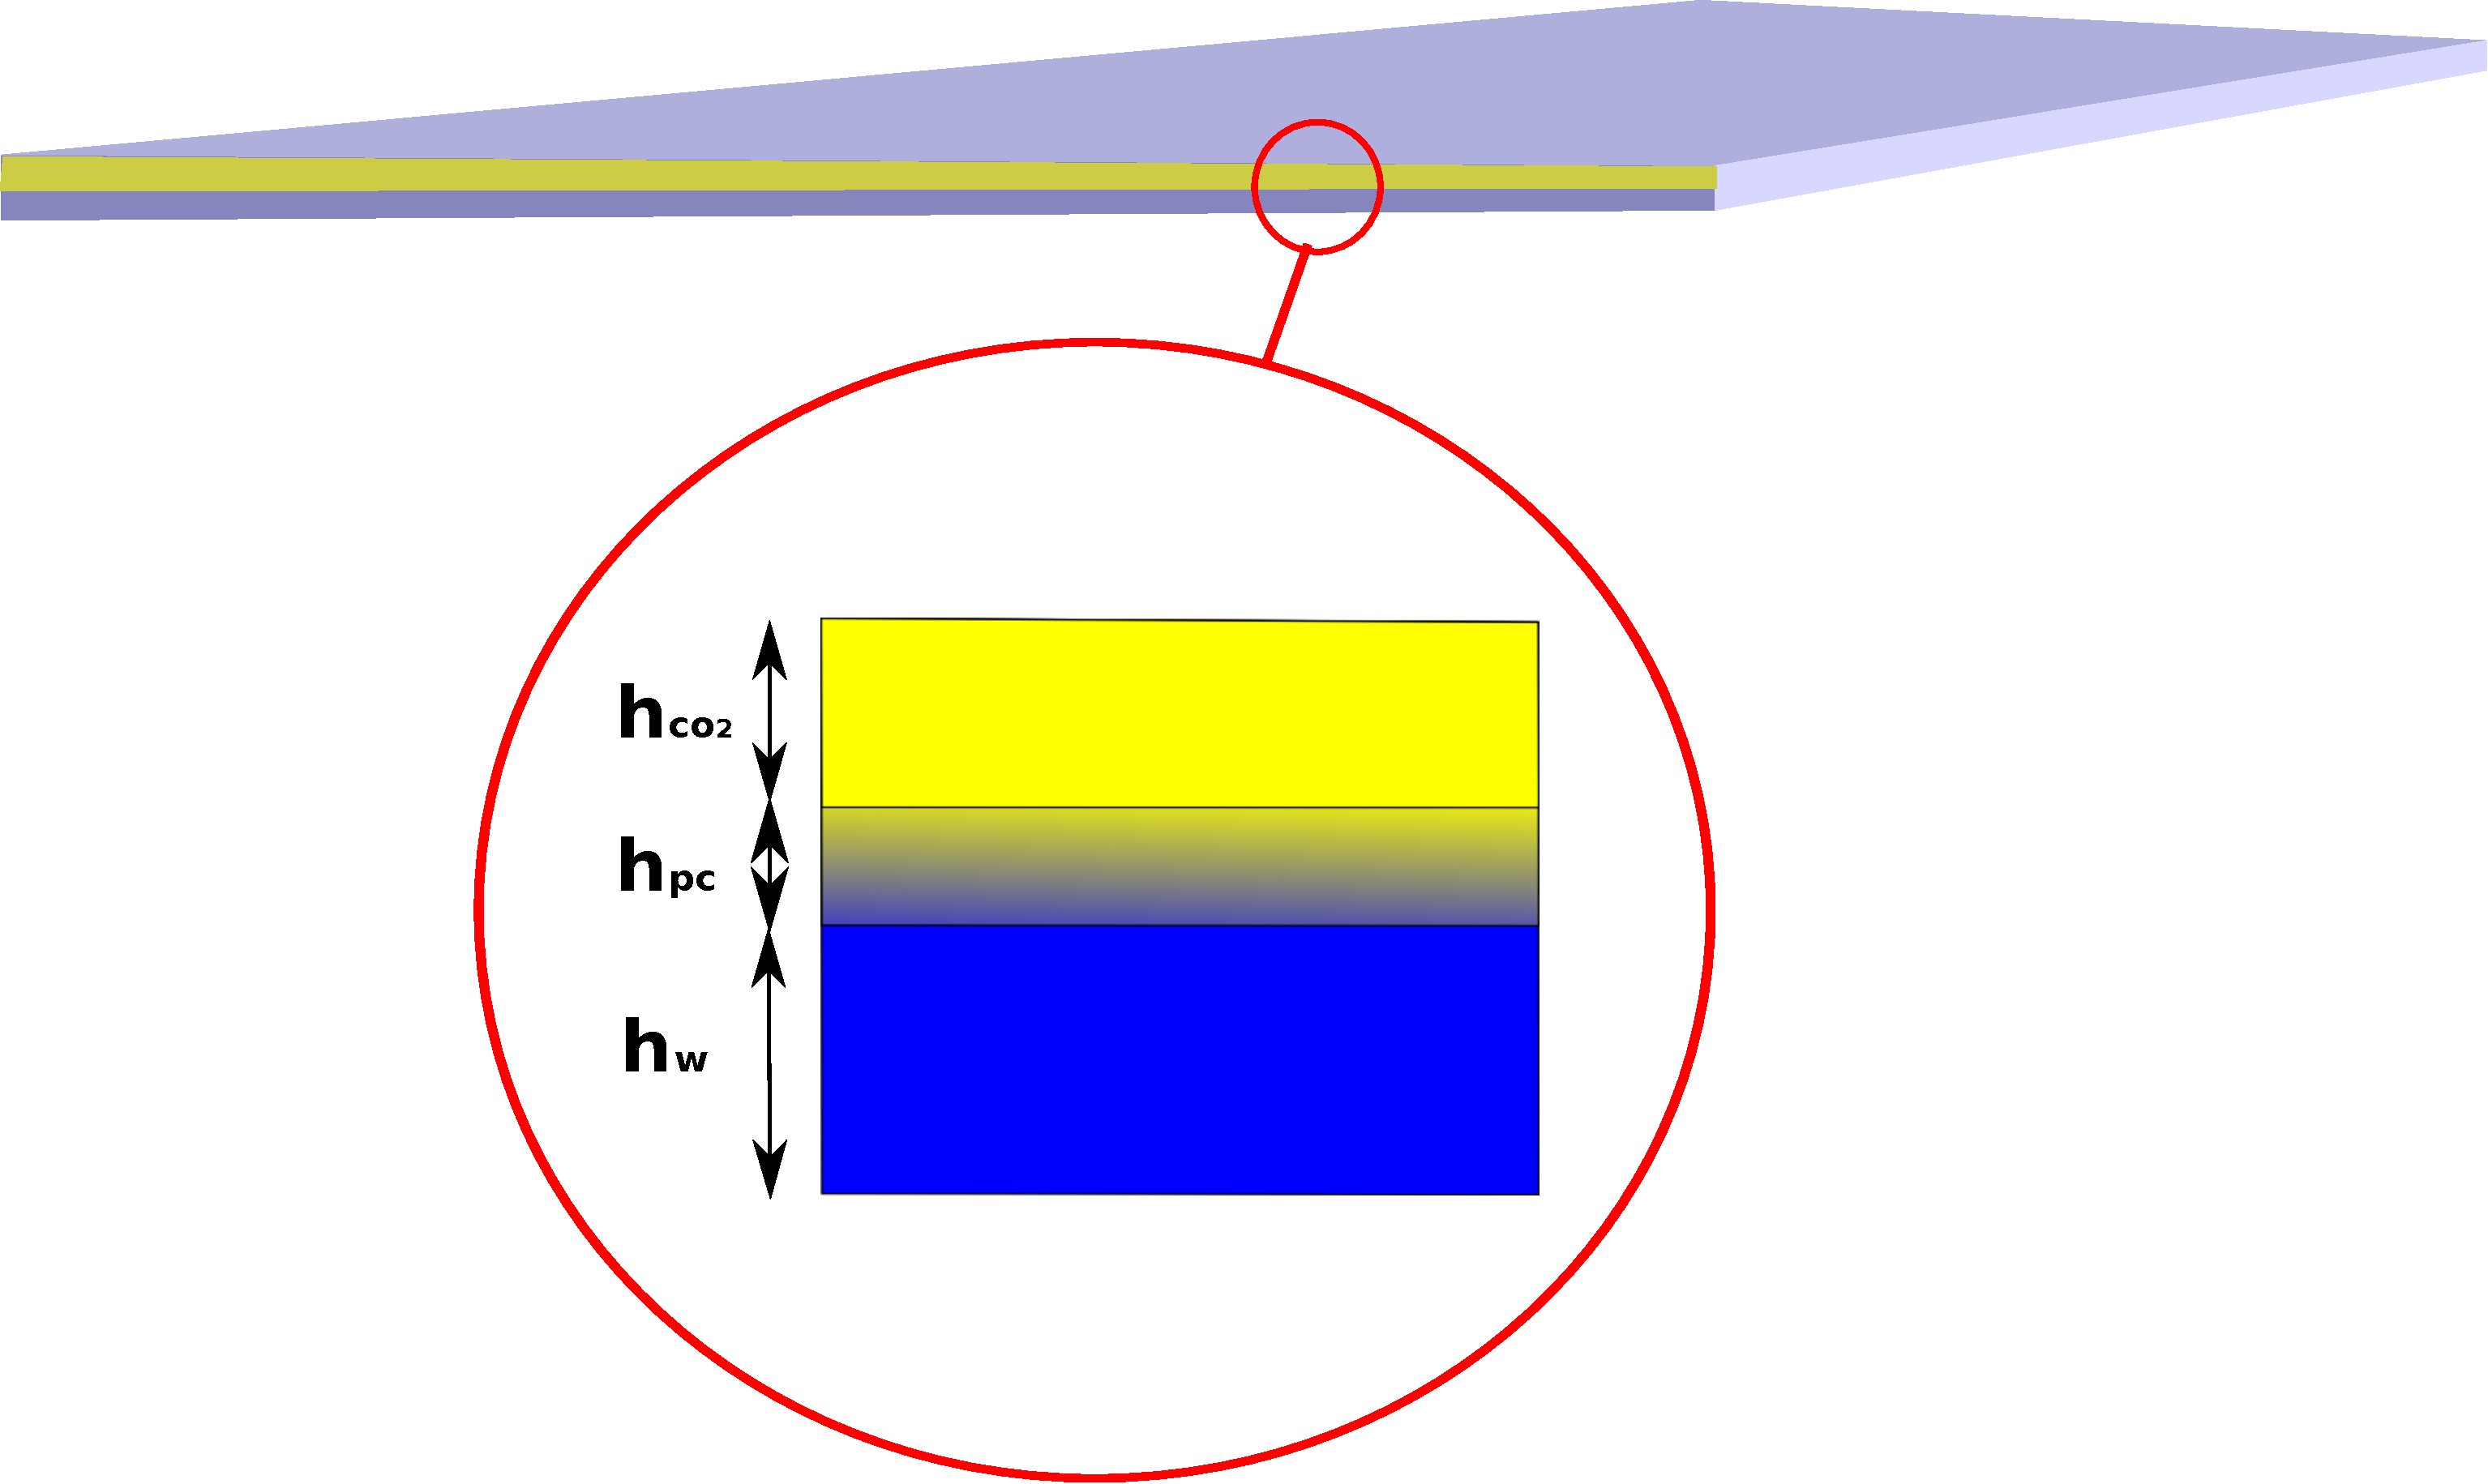
\includegraphics[width=1\linewidth]{./figurer/VACOL}
 \caption{Hydrostatic equilibrium condition results in three zones:
the $\mbox{CO}_2$ zone with thickness $h_{co_2}$, the water table with thickness
$h_{w}$, and the capillary transition zone $h_{pc}$.}
 \label{fig:VC}
\end{figure}


Accuracy of vertical averaging approach within $\mbox{CO}_2$ storage context has
been
examined in many works in the literature
\cite{moll2011field,lie2010accurate,class2009benchmark,grayderivation}. It has
been shown that vertical averaging is applicable to large scale $\mbox{CO}_2$
studies. The numerical aspects and speed up of the method compared to three
dimensional problem are studied in
\cite{ligaarden2010numerical,grayderivation}, where a second order
speedup is reported. Lie et al. \cite{lie2010accurate} have shown the
influence of vertical discretization in the three dimensional models which can
fail in low resolutions to capture the thin layer of $\mbox{CO}_2$ plume
migrating beneath the top sealing surface in the formation. The vertical
averaging approach can handle this issue by considering the water and
$\mbox{CO}_2$ interface in calculating the vertically averaged parameters in the
model. A comparison between three and two dimensional models has been done on
various aspects in \cite{moll2011field}.

The influence of topography in modeling the $\mbox{CO}_2$ migration
and estimating the storage fate has been shown in
\cite{syversveenstudy,grayderivation} by examining different geometries and
heterogeneities in the domain. These conclusions suggest that the significance
of the model top surface is more than the small order flow in the model vertical
thickness.

The studies reported in this thesis concern the flow near injector and early
times of plume development. Therefore vertical equilibrium would benefit larger
scales with big portion of model in vertical equilibrium. We do our flow
modeling by including the three dimensions and for the quantitative uncertainty
analysis we employ a polynomial approximation (Section
\ref{sec:StochasticAnalysis}).

\section{Flow modeling}
\label{sec:FolowModeling}

We use a standard porous media simulator \cite{sis2007eclipse} to solve the flow equations in the
medium. The simulator is based on finite volume method and the following
assumptions are taken:

\begin{itemize}

  \item Two compressible phases are considered in the medium: water and super
critical ${CO}_2$.
  \item No mass exchange occurs between the two phases.
  \item No heat exchange is considered.
 
\end{itemize}

\subsection{Numerical scheme}

The simulator uses a standard two-point finite difference scheme to solve
Equation \ref{eq:dif2p} on a corner-point grid. The Darcy equation for two-phases can be written in a difference. This makes the flow equation into cell $a$ from the
neighboring cell $b$:
\begin{equation}
 F_{ab\alpha}=T_{ab}M_{a\alpha}\Delta \psi_{\alpha}.
\label{eq:eclF}
\end{equation} Here, $T_{ab}$ is the transmissibility of the medium between the two cells. $M_{a\alpha}$ is the mobility of phase $\alpha$ that is taken upstream of the flow from cell ${a}$ and $\Delta \psi_{\alpha}$ is the potential term difference between two cell centers. 


\begin{figure}
 \centering{}
 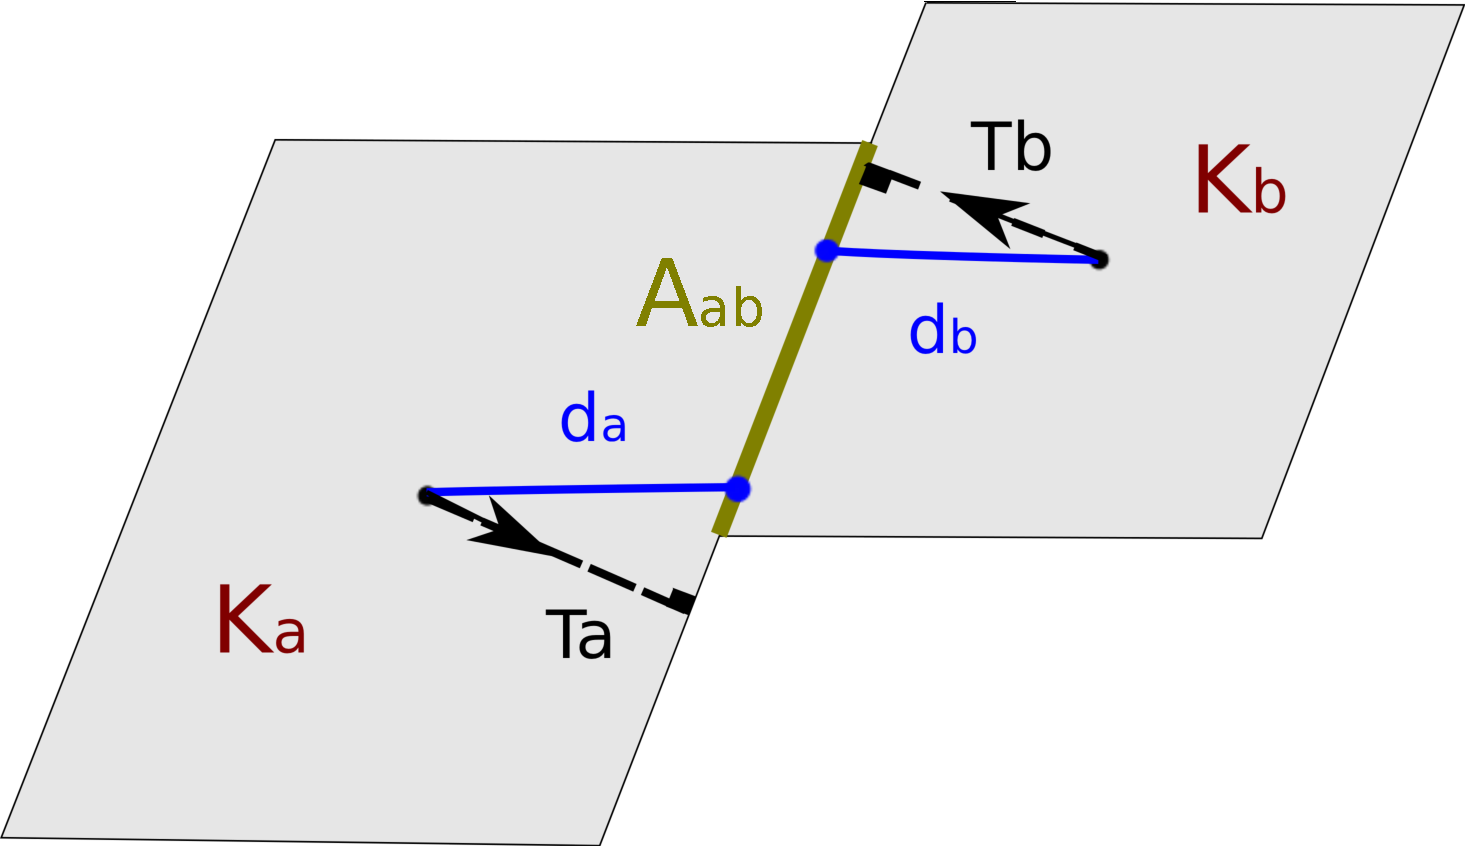
\includegraphics[width=0.4\linewidth]{./figurer/trans}
 \caption{Transmissibility calculation for two cells $\mbox{a}$ and $\mbox{b}$.}
 \label{fig:tran}
\end{figure}

Transmissibility for two neighboring cells (i.e., sharing a face area, see
Figure \ref{fig:tran}) is
calculated by harmonic average of transmissibilities from the center of each
cell to the center of the common face between the two cells:
\begin{equation}
 T_{ab}=\frac{1}{\frac{1}{T_a}+\frac{1}{T_b}}.
 \label{eq:Thav}
\end{equation} Each half transmissibility $T_{a}$ or $T_{b}$ is calculated by an inner product
between the permeability of the cell $K_a $, the mutual area $A_{ab}$ between cells, and the distance from cell center to the mutual face center $d_a$:
\begin{equation}
  T_a = K_a \cdot d_a \cdot A_{ab}.
  \label{eq:tran}
\end{equation}

The mobility term in Equation \ref{eq:eclF} is defined as follows:
\begin{equation}
 M_{a\alpha}=\frac{k_{r\alpha}}{B_\alpha \mu_\alpha},
 \label{eq:mob}
\end{equation} where $k_{r\alpha}$ is the relative permeability of phase
$\alpha$, $\mu_\alpha$ is the viscosity of phase $\alpha$, and $B_\alpha$ is the
formation volume factor of phase $\alpha$, which is defined as :
\begin{equation}
 B_\alpha=\frac{\mbox{Volume at surface condition}}{\mbox{Volume at formation
condition}}=\frac{V_{s\alpha}}{V_{r\alpha}}.  
\end{equation} This definition is connected to compressibility
of the fluid, i.e., to changes in volume at surface and at the geological formation condition, but it is defined in this way in the simulator to honor cases where a
fluid like oil loses its dissolved gas while being produced at surface pressure.
Since we assume no mass exchange between phases in our study, here the formation
volume factor works like compressibility of the fluid. Formation volume factor
is a function of pressure. Slight compressibility is considered for phases in our study, and phase density
is defined as a function of pressure:
\begin{equation}
 \rho_\alpha(P) =\frac{\rho_{0\alpha}}{B_\alpha(P)}.
 \label{eq:rho}
\end{equation} Here, $\rho_{0\alpha}$ is the density of phase $\alpha$ at
surface condition.

Wells are defined as sources or sinks in Equation \ref{eq:dif2p}. In reality, wells
are a void space drilled in the porous medium and the flow into the
well-bore and up to the surface for production wells (and vice-versa for injectors)
goes through a pressure change that must be modeled separately from the porous
medium. 


\begin{figure}
 \centering{}
 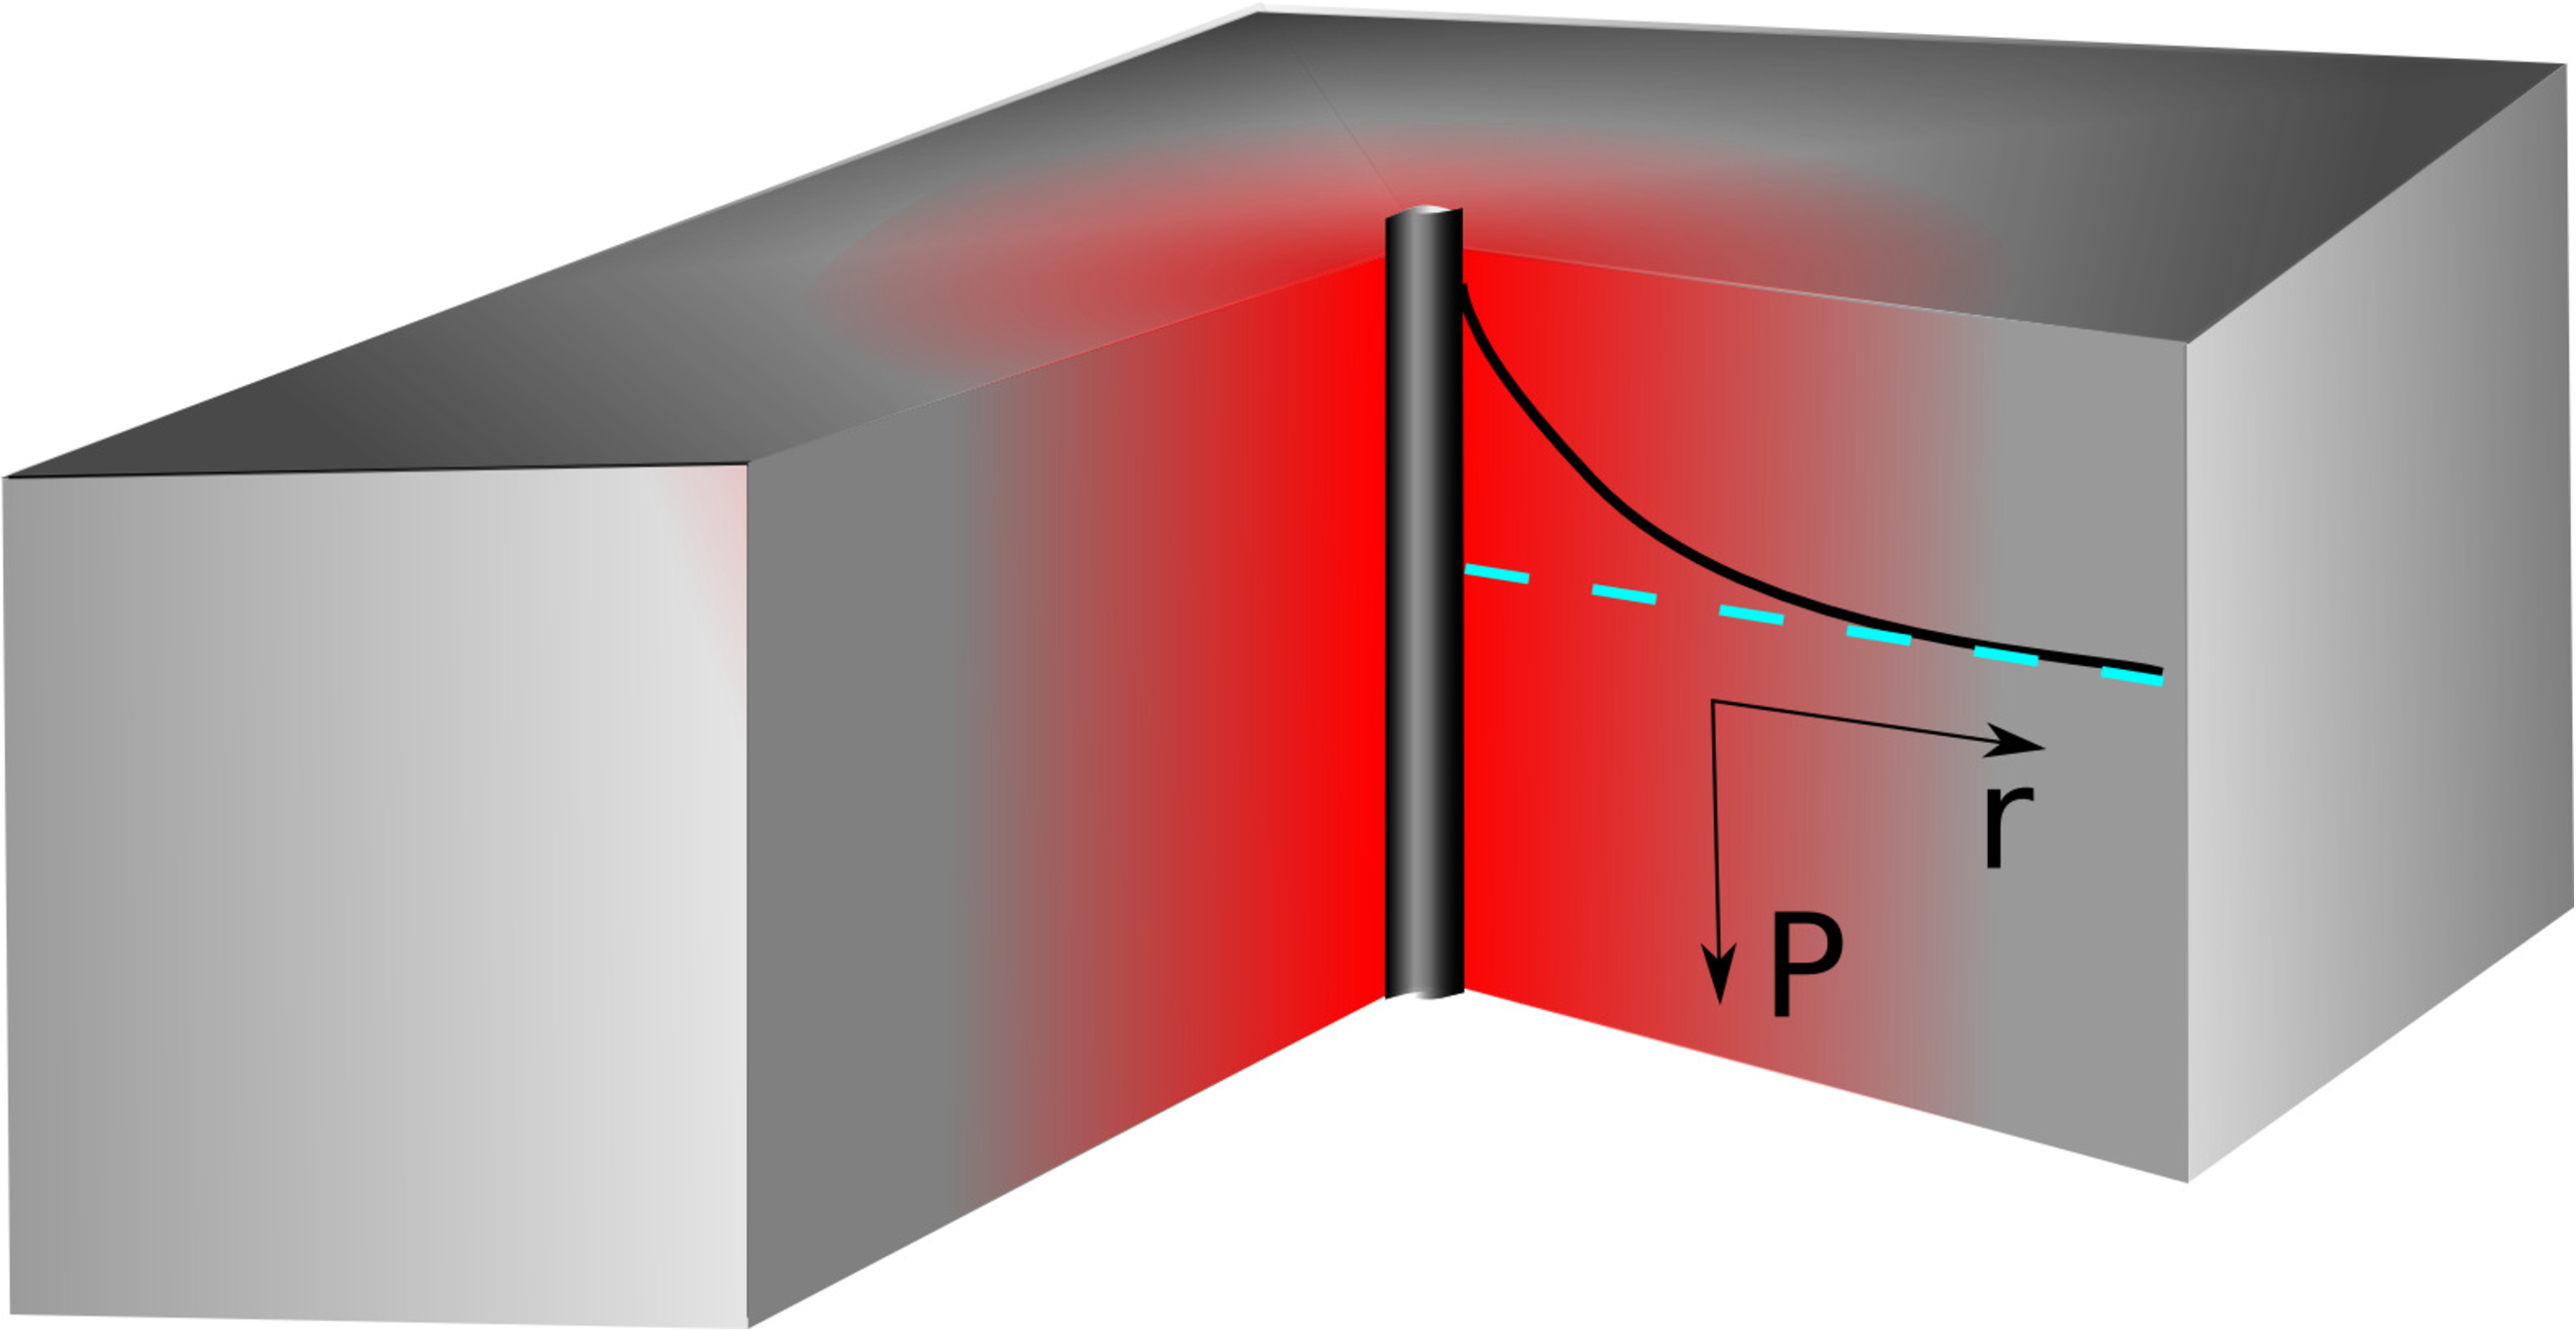
\includegraphics[width=0.4\linewidth]{./figurer/WModel}
 \caption{Well modeling inside a simulation cell.}
 \label{fig:WM}
\end{figure}

Figure \ref{fig:WM} shows a schematic pressure distribution around the
injector. The well radius is much smaller than the simulation cell containing
the well and the pressure in the bottom-hole is different than the cell
pressure. The well bottom-hole pressure can be related to the cell pressure
containing the well by a separate approximation that can be coupled with the
flow equations in the grid model. Flow equation for phase $\alpha$ between the
cell center and the well for an injector is written as follows:

\begin{equation}
 \eta_{\alpha}=T_w\cdot M_{\alpha}\cdot [P_w-P_{{i}}].
 \label{eq:WFLW}
\end{equation} Here, $\eta_{\alpha}$ is the volumetric injection rate of phase
$\alpha$, $P_w$ is the injector bottom-hole pressure, $P_{{i}}$ is the
cell pressure, $T_{w}$ is the transmissibility between the cell and the
injection well-bore, and $M_\alpha$ is the mobility of injection flow into the
cell. 

A region can be assumed by a radius $r_e$ at which the
pressure is equal to the cell pressure. Approximating the flow near the
well-bore by Equation \ref{eq:vol}, the transmissibility for this region can be
found from the analytical solution to Equation \ref{eq:vol}:
\begin{equation}
 T_w=\frac{K \cdot h}{ln(\frac{r_e}{r_w})},
 \label{eq:Tw}
\end{equation} where $h$ is the medium
thickness, $K$ is the medium rock permeability, and $r_{w}$ is the well radius. Here, we assume that the well is completed and connected in the entire thickness $h$ of the cell and there is no skin effect in the well. The Equation \ref{eq:Tw} can be extended to model wells with partial completions and skins. The effective radius $r_{e}$ in Equation \ref{eq:Tw} is estimated from Peaceman formula and can be related to the cell geometry:
\begin{equation}
r_e =  0.28\frac{\left[
\delta_x^2(\frac{K_y}{K_x})^{\frac{1}{2}}+\delta_y^2(\frac{K_x}{K_y})^{\frac{1}{
2}}\right]^{\frac{1}{2}}}{(\frac{K_y}{K_x})^{\frac{1}{4}}+(\frac{K_x}{K_y})^{
\frac{1}{4}}}.
\label{eq:rinf} 
\end{equation} Here, $K_x$ and $K_y$ are the permeabilities in $x$ and $y$
directions and $\delta_x$ and $\delta_y$ are the cell sizes in these directions.
This equation assumes a vertical well and a diagonal permeability tensor. It can
be modified for more general cases.

\subsection{Flow scenarios}

% All of the SAIGUP realizations have dimensions of
% $3~\mbox{km}~\times~9~\mbox{km}~\times~80~\mbox{m}$, which is enough to capture
% variations in the designed geological features. While the volume of the
% realizations is large enough to capture major parts of the injected volume, the
% pressure disturbance imposed by the injector can go beyond this
% scale. To compensate for the size, we choose hydrostatics boundary conditions
% for the models. The open boundaries are modeled by considering a huge pore
% volume for the outer cells in the model that represent the boundary. Figure
% \ref{fig:BDRY} shows the boundary condition defined in the model. 

All of the SAIGUP realizations have dimensions of $3~\mbox{km}~\times~9~\mbox{km}~\times~80~\mbox{m}$. The model spatial scales capture the typical geological features in a shallow-marine system, such as shore-line shape and aggradation angle variations. Various scales of heterogeneity can considerably impact the flow behavior. The considered grid resolution in the lateral dimension is appropriate for simulating the interaction of the heterogeneities in the medium with the \coo\ plume.  However, in the vertical scale the study can be improved by using a higher grid resolution. Variations in the vertical direction exist in considerably smaller scales than the lateral direction. In particular, this is more crucial for the long-term migration of \coo\, where  a thin plume of \coo\ migrates beneath a sealing layer due to the buoyancy forces.

The model dimensions are appropriate for studying the spatial distribution of \coo\ in the medium during injection and early migration periods. However, a detailed pressure study requires larger scales than what is used here. Flow analysis on the SAIGUP scale indicates that some of the geological parameters are more influential for the pressure response than others. We investigate the operational concerns  related to pressure build-up for typical injection scenarios and we develop mitigation plans in our study. However, the conclusions on pressure response sensitivity to geological parameters are more qualitative and instructive. Though, we perform an extensive probabilistic analysis on the \coo\ pressure behavior in the medium that can be applied in a further study with specific concerns about the pressure analysis.   

The choice of open boundary is not valid in domains that are bounded by structural seals. In fact, for the close and semi-close domains the pressure is a main control on the storage capacity along with other parameters. We assume open boundaries, and the results of our study can change significantly by choosing different boundary condition. On the other hand, representing the boundary by large pore volumes on the outer closed cells makes the pressure to relax earlier than it does in a large infinite domain. Therefore, the pressure responses in our study, which are already extreme in many cases due to heterogeneity, can be magnified when it is run in huge sized models.

We consider the injection of $20\%$ of the total pore volume of the model(excluding the large volumes at the boundaries), which amounts to $40~\mbox{MM m}^3$. This volume is injected into all realizations
in three different scenarios. In the first scenario, the injection is forced to
finish in
$30~\mbox{years}$ and the pressure in the system is allowed to rise
unlimitedly. Linear relative permeability functions are considered in this
scenario. The purpose of the first scenario is to examine the flow distribution in the medium influenced by geological heterogeneity. Linear assumption for
relative permeabilities is taken to speed up the flow within the medium. The
relative permeability curvature has shown a significant influence on the
pressure behavior during \coo\ injection into the  aquifer. However, \coo\ moving under a cap-rock will effectively have a linear relative permeability.

In the second scenario, the injector operates with the same fixed rate as in the
first scenario and the relative permeability curves are chosen to be quadratic
functions. Quadratic relative permeability curves cause lower flow mobility in
the medium compared to the linear function, and by forcing the injector with a
fixed volumetric rate of injection, the pressure rises significantly in the
aquifer. This leads us to the third injection scenario, where the injector is
controlled by pressure rather than volumetric rate. Thus, injection time is
variable depending on the injectivity of the medium.

Only one injector is considered in the study. With one injector, it is easier to
study the flow behavior and the plume development within the medium. The
injector is
located in the flank and to increase the sweep efficiency for the
up-moving $\mbox{CO}_2$ plume, the injector is completed only in the lower part
of
the aquifer. The injector location and the completed layers are fixed for all of
the realizations. The studies here aim to identify the influence of uncertainty
on injectivity and fixing a place for injection helps in achieving this goal. As mentioned earlier, injectivity is a big player in the success of the operations. Uncertainty might be less in the near well-bore region than in the larger scale in the domain, but yet requires costly operation data aquisition. Fixing the location of the well serves specifiying the probability of having a feasible injectivity in different heterogeneities.

There are few locations of distorted geometries in the faulted realizations that
may be considered as structural traps for the injected $\mbox{CO}_2$. The
topography in the SAIGUP realizations is simple and does not cover the
variational space to be used in a sensitivity analysis. The slight inclination
in the structural geometry of the medium, from the flank up to the crest, leads
the injected $\mbox{CO}_2$  to accumulate in the crest and below the faulted
side of the aquifer. The structural trapping due to variational morphology is
studied in IGEMS, which is a sister project to MatMora (for example, see
\cite{syversveenstudy}). 

In a homogeneous medium, we expect the $\mbox{CO}_2$ to accumulate under the
cap-rock. A small fraction of the injected $\mbox{CO}_2$ will escape through the
open boundary near the injection well and the rest of it will stay within the
medium in two forms that we refer to as  mobile and residual volumes. As
the $\mbox{CO}_2$ moves through the rock, part of it stays in the smaller pores
by capillary trapping process and can not be discharged by brine. The other
parts move through the larger pores and can be displaced by water in an
imbibition process. This volume is called mobile. As we are interested in
storing the $\mbox{CO}_2$ permanently and safely, increasing the trapped volume
is in line with the objective of minimizing the leakage risk and maximizing the
storage capacity. Likewise, the more mobile volume of $\mbox{CO}_2$ exists in
the medium, the more will be the risk of leakage. 

\begin{figure}
 \centering{}
 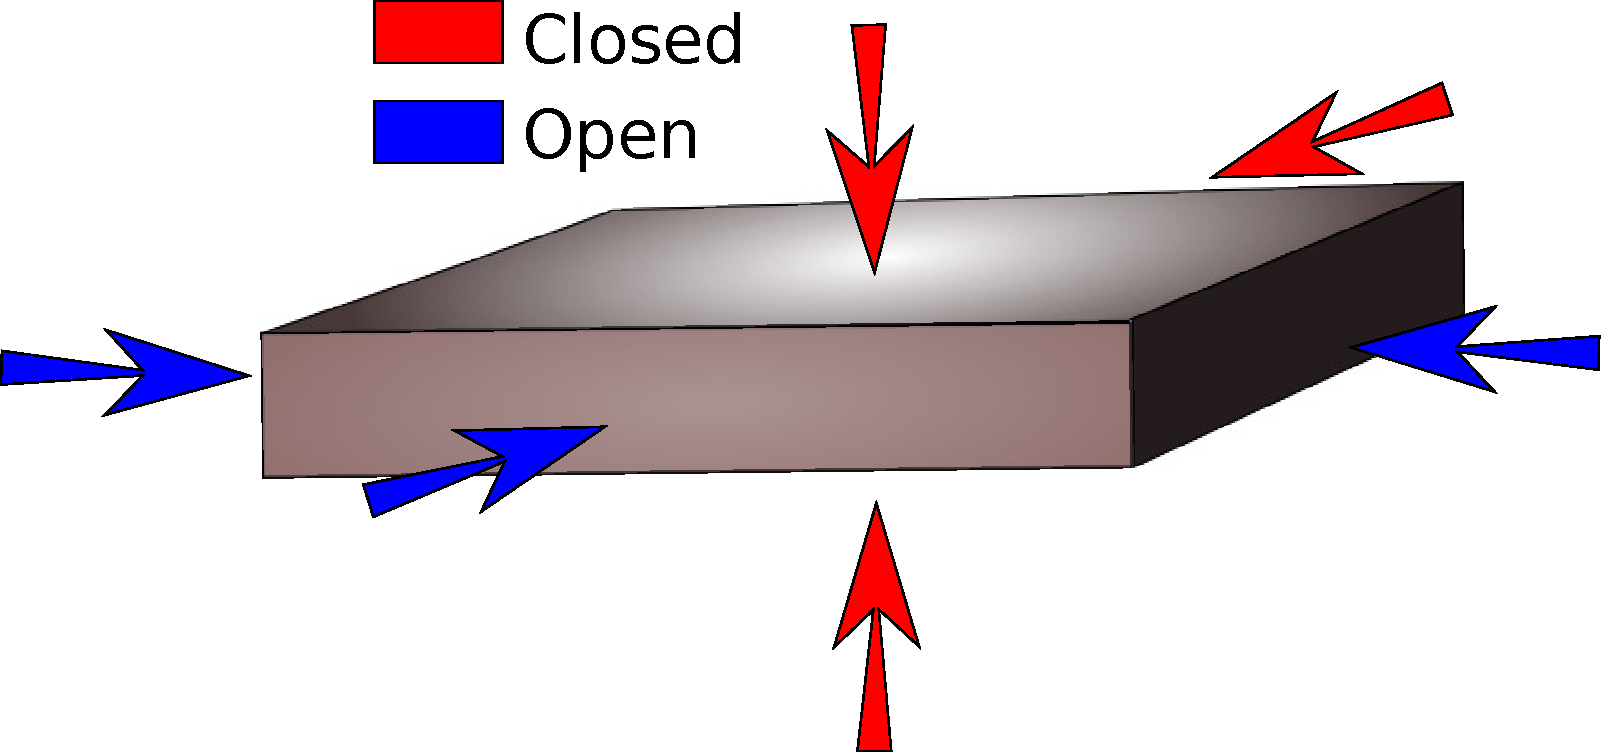
\includegraphics[width=0.6\linewidth]{./figurer/boundaries}
 \caption{Top, bottom, and upper side boundaries are closed and the rest
are open to the flow.}
 \label{fig:BDRY}
\end{figure}

Defining the boundary condition of the aquifer of interest can influence the
flow behavior in the system. Computational costs make it more feasible to model the flow locally and in the
part of the aquifer that is going through more pronounced changes in flow
behavior. Therefore, we can choose the boundaries of the model inside the aquifer
in a volume that is containing the injection wells and the areas effected by
them. Hydrostatic open boundary condition is a choice for the system boundaries
to include the aquifer parts that fall outside the boundaries (Fig.
\ref{fig:bkw}).

The underground network of aquifer systems can be connected via geological
channeling and conductive features. Some aquifers might be active and connected
to the surface and expand in volume by variations in water influx due to 
seasonal rains. This can impose an external force on the system boundaries
considered in a storage problem. Fig. \ref{fig:bkw} shows the water influx
through the boundaries of the system due to external aquifer activities. We
consider the external support by imposing a higher pressure than the hydrostatic
pressure on the boundary of the model.

\begin{figure}[thb]
  \centering
  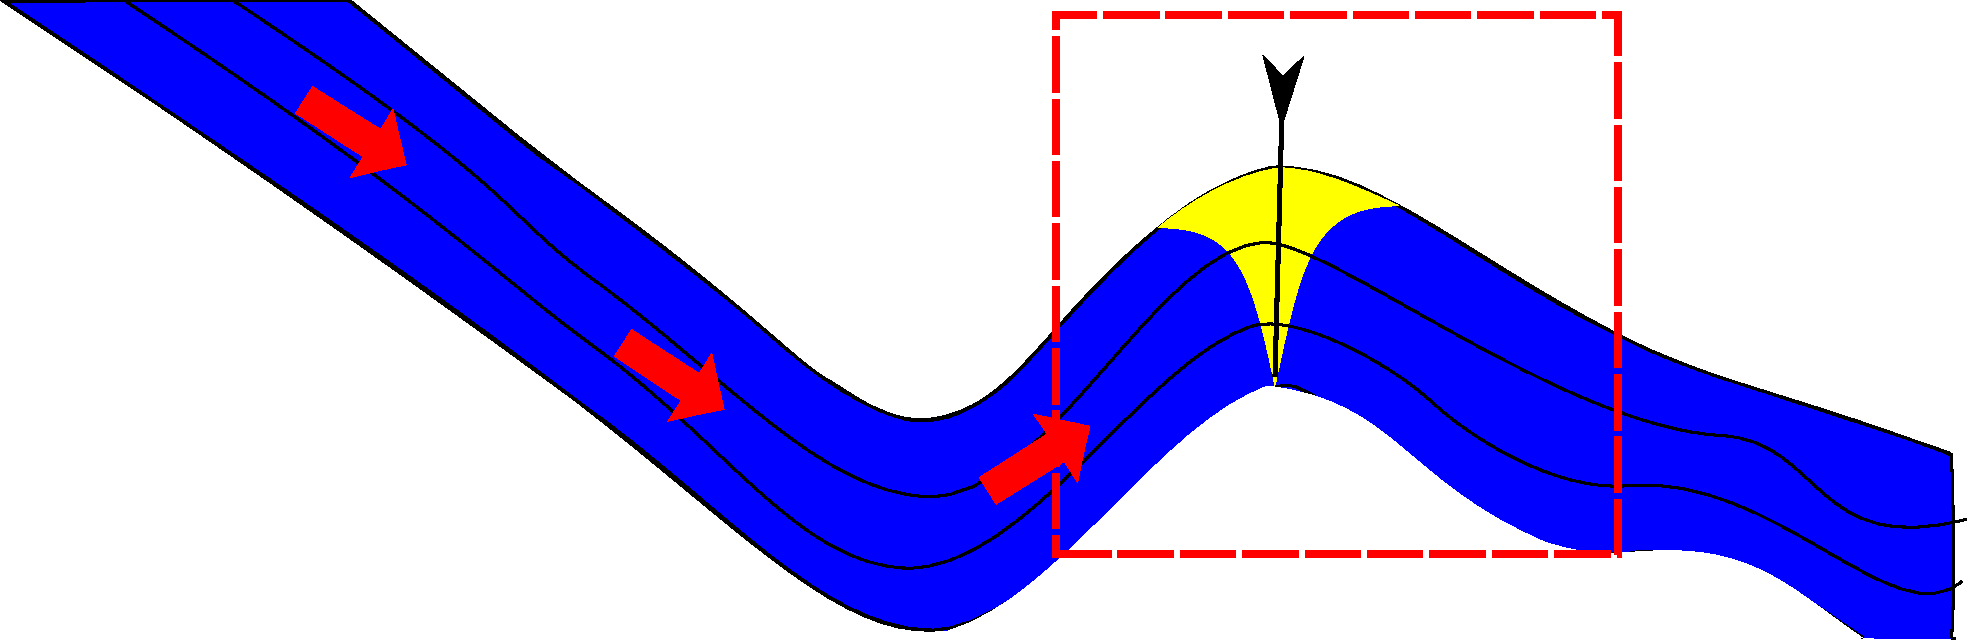
\includegraphics[width=0.65 \linewidth]{./figurer/bkw} 
  %
  \caption{External pressure drive.}
  \label{fig:bkw}
%
\end{figure}


\subsection{Flow responses}

The primary unknowns in the flow model are the $\mbox{CO}_2$ pressure
and the saturation distribution at different times. From the simulation
output, we can derive quantities that
address the feasibility of $\mbox{CO}_2$ injection,
these quantities include a number of flow responses related to the $\mbox{CO}_2$
injection and migration problems. Each of these responses are directly or
indirectly a measure of success for the operation within a specific realization.
In the following, we give a brief description of each of them:

\textbf{\textit{Boundary fluxes:}} The flux out of open boundaries is a measure
of sweep efficiency for the
CO$_2$ plume. Channeling can lead to early CO$_2$ breakthrough at boundaries and
we prefer cases with less out-fluxes through open boundaries. The out-flux
through the open boundary that is closer to the injector is a potential
loss for the injected volume. After the injection stops, some of the CO$_2$ that
has left the domain comes in again due to gravity segregation effect. 

\textbf{\textit{Total mobile and residual $\mbox{CO}_2$ volume:}}
If the CO$_2$ saturation is below the critical value, it will be immobile in the
bulk flow, although not in the molecular sense. Less mobile CO$_2$ means less
risk of leakage and more residual volumes (with saturations less than the
critical) resulting from a more efficient volume sweep as preferable. We use
critical saturation of 0.2 for both water and CO$_2$. During injection time the
flow process is mainly drainage but after injection imbibition also happens and
increases the residual trapped CO$_2$. 

\begin{figure}[thb]
  \centering
  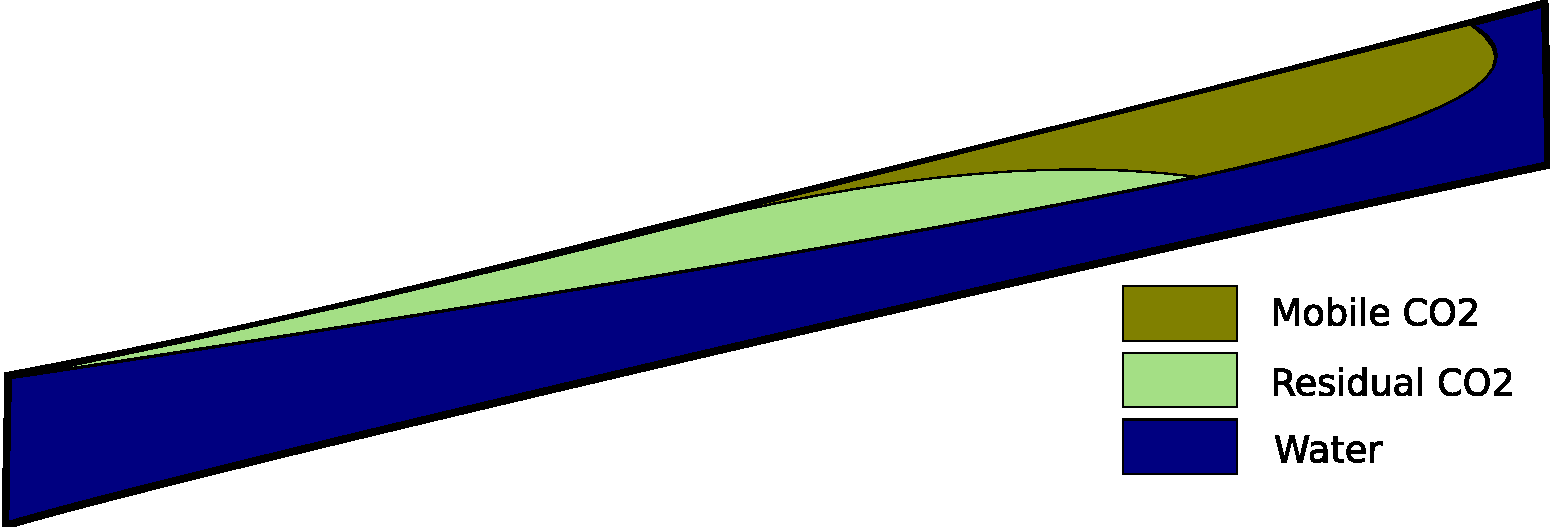
\includegraphics[width=0.65 \linewidth]{./figurer/MobRes} 
  %
  \caption{Mobile and residual CO$_2$ volume.}
  \label{fig:MobRes}
%
\end{figure}

\textbf{\textit{Total number of $\mbox{CO}_2$ plumes and largest plume:}} To
estimate the risk of leakage from the cap-rock, we assume that all mobile
CO$_2$ connected to a leakage point will escape out of the reservoir. Hence, it
is preferable if the total mobile CO$_2$ volume is split into smaller plumes
rather than forming a big mobile plume. We looked at the largest plume size, the number of
plumes, and other statistical parameters. 

% 
% \begin{figure}[thb]
%   \centering
%   \includegraphics[width=0.65 \linewidth]{./figurer/NWB} 
%   %
%   \caption{NWB.}
%   \label{fig:nwb}
% %
% \end{figure}

\textbf{\textit{Average aquifer pressure:}} Average aquifer pressure is one of
the most important responses to be
considered. The pressure response in general shows a sharp jump at the start of
injection and a declining trend during the injection and plume migration.  

As soon as the injection starts, a pulse of pressure goes through the
medium, introducing
a pressure buildup in the aquifer. When the pressure wave reaches the open
boundary, the aquifer pressure starts declining to a level maintained by the
injector. When the injector stops operation, the pressure support will be
removed and the pressure drops and declines until it reaches equilibrium.

\textbf{\textit{Leakage risk:}} During injection operation the foremost
important issue is the aquifer pressure
which as discussed earlier may lead to fractures in the cap-rock. On the other
hand, the cap-rock break depends on lithology and sealing thickness and differs
from point to point. Some weaker locations can be the most probable to
break and start leaking if any mobile CO$_2$ exists there.

An uncertainty assessment process consisting of geo-mechanical modeling of aquifer combined with flow modeling can cost a large amount of computations. To avoid expensive computations, the idea in this thesis is to model the possible breakings on the cap-rock (considering the stress stream in the medium) by introducing a probability measure on the cap-rock. This measure can be used to
evaluate different cases for their risk of leakage, considering the CO$_2$
distribution under the cap-rock. 

Here, we define the probability of leakage as a measure on the cap-rock that
assigns a value to each point of the cap-rock, modeling the relative weakness of
the cap-rock and the medium at that point. If for example both the cap-rock and
the aquifer are continuous homogeneous layers with constant thickness, then the
point of cap-rock that sits on the highest point of the injection slice can be
the most probable place for leakage in case of dramatic pressure increase in the
well: the stress stream is more in the injection slice and the CO$_2$
accumulation occurs on the topmost part of the mentioned slice. Then one may
consider a 2D-Gaussian probability distribution on the cap-rock, centered above
the injection slice.

If the medium is heterogeneous or tilted, the injected CO$_2$ may be distributed
in different number and sizes of plumes below the cap-rock. Therefore, in
addition to the probability of breaking for each point of cap-rock, one must
consider the CO$_2$ connected volume that is attached to that point. 

Since we have neither the cap-rock model nor the geo-mechanical properties of
the SAIGUP models, we use a simple 2D-Gaussian leakage probability distribution
centered at a point on the crest which is in the same slice as the injection
point (Fig. \ref{fig:SLR}). We calculate the probability of each cell in the top
layer and using the simulation results for the case, we weight it by the CO$_2$
saturation of that cell and the plume size that the cell is attached to.
Summing up the values of the topmost cells, we assign a single number to the
case which we call leakage risk of the case. One may weight the case risk value
with the average pressure in the system, such that higher pressure gives a
bigger weight.
\vskip 0.5cm

\begin{figure}
  \centering
  \includegraphics[width=0.65 \linewidth]{./figurer/LR_2} 
  %
  \caption{We use a $2\mbox{D}$ Gaussian distribution for leakage probability
on the cap-rock.}
  \label{fig:SLR}
%
\end{figure}

Results are discussed by comparing all cases in plots. However, the conclusions are made based on detailed flow study in some picked cases. For example, Figures \ref{fig:Kz} to \ref{fig:FOSEOI} show the rock properties and \coo\ distribution in the domain at end of injection and end of simulation in two different cases. The heterogeneity description of the selected cases, called A and B, is given in Table \ref{tab:AaB}.

\coo\ distribution in Figures \ref{fig:COEOI} and \ref{fig:COEOS} show that heterogeneity in case B has enhanced the lateral flow compared to case A. Direction of the flow can be seen in Figure \ref{fig:FOSEOI}. It is clear that heterogeneity can influence the imbibition and drainage process during and after injection. This, in turn, impacts the residual trapping process.

\begin{table}
\center
\caption{Geological heterogeneities for two selected cases.}
\begin{tabular}{|c|||c||c||c|||c||c|}
\hline
Case & Fault&Lobosity&Barrier&Aggradation Angle&Progradation Direction\\
\hline
A&unfaulted&medium&medium&medium&down-dip\\
\hline
B&unfaulted&high&medium&low&up-dip\\
\hline
\end{tabular}
\label{tab:AaB}
\end{table}
%===> 

\begin{figure}
\begin{tabular}{cc}
\includegraphics[width=0.45\textwidth]{./figurer/C02222_LogKz_pers}&
\includegraphics[width=0.45\textwidth]{./figurer/C03211_LogKz_pers} \\ \hline  
(a) Perspective view of model A&(b) Perspective view of model B\\
\includegraphics[width=0.45\textwidth]{./figurer/C02222_LogKz_slcx}&
\includegraphics[width=0.45\textwidth]{./figurer/C03211_LogKz_slcx}
\\(c) The X slice at the injection point (see (a)).&
(d) The X slice at the injection point (see (b)).\\
\includegraphics[width=0.45\textwidth]{./figurer/C02222_LogKz_slcy}&
\includegraphics[width=0.45\textwidth]{./figurer/C03211_LogKz_slcy}
\\(e) The Y slice at the injection point (see (a)).&
(f) The Y slice at the injection point (see (b)).
\end{tabular}
\caption{Transmissibility in the vertical direction for two selected cases. The left plots correspond to case A in Table \ref{tab:AaB}, and the right plots belong to case B. Colors are in log scale and the scale in Figures (a) and (b) are powers of ten in cP$.$m$^3$/day/bar units.}
\label{fig:Kz}
\end{figure}

\begin{figure}
\begin{tabular}{cc}
\includegraphics[width=0.45\textwidth]{./figurer/C02222_LogKy_pers}&
\includegraphics[width=0.45\textwidth]{./figurer/C03211_LogKy_pers}
\\(a) Perspective view of model A&(b) Perspective view of model B\\
\includegraphics[width=0.45\textwidth]{./figurer/C02222_LogKy_slcx}&
\includegraphics[width=0.45\textwidth]{./figurer/C03211_LogKy_slcx}
\\(c) The X slice at the injection point (see (a)).&
(d) The X slice at the injection point (see (b)).\\
\includegraphics[width=0.45\textwidth]{./figurer/C02222_LogKy_slcy}&
\includegraphics[width=0.45\textwidth]{./figurer/C03211_LogKy_slcy}
\\(e) The Y slice at the injection point (see (a)).&
(f) The Y slice at the injection point (see (b)).
\end{tabular}
\caption{Transmissbility in the lateral direction for two selected cases. The left plots correspond to case A in Table \ref{tab:AaB}, and the right plots belong to case B. Colors are in log scale and the scale in Figures (a) and (b) are powers of ten in cP$.$m$^3$/day/bar units.}
\label{fig:Ky}
\end{figure}

\begin{figure}
\begin{tabular}{cc}
\includegraphics[width=0.45\textwidth]{./figurer/C02222_CO2atEOI_pers}&
\includegraphics[width=0.45\textwidth]{./figurer/C03211_CO2atEOI_pers}
\\(a) Perspective view of model A&(b) Perspective view of model B\\
\includegraphics[width=0.45\textwidth]{./figurer/C02222_CO2atEOI_slcx}&
\includegraphics[width=0.45\textwidth]{./figurer/C03211_CO2atEOI_slcx}
\\(c) The X slice at the injection point (see (a)).&
(d) The X slice at the injection point (see (b)).\\
\includegraphics[width=0.45\textwidth]{./figurer/C02222_CO2atEOI_slcy}&
\includegraphics[width=0.45\textwidth]{./figurer/C03211_CO2atEOI_slcy}
\\(e) The Y slice at the injection point (see (a)).&
(f) The Y slice at the injection point (see (b)).
\end{tabular}
\caption{\coo\ distribution at the end of injection for two selected cases. The left plots correspond to case A in Table \ref{tab:AaB}, and the right plots belong to case B.}
\label{fig:COEOI}
\end{figure}

\begin{figure}
\begin{tabular}{cc}
\includegraphics[width=0.45\textwidth]{./figurer/C02222_CO2atEOS_pers}&
\includegraphics[width=0.45\textwidth]{./figurer/C03211_CO2atEOS_pers}
\\(a) Perspective view of model A&(b) Perspective view of model B\\
\includegraphics[width=0.45\textwidth]{./figurer/C02222_CO2atEOS_slcx}&
\includegraphics[width=0.45\textwidth]{./figurer/C03211_CO2atEOS_slcx}
\\(c) The X slice at the injection point (see (a)).&
(d) The X slice at the injection point (see (b)).\\
\includegraphics[width=0.45\textwidth]{./figurer/C02222_CO2atEOS_slcy}&
\includegraphics[width=0.45\textwidth]{./figurer/C03211_CO2atEOS_slcy}
\\(e) The Y slice at the injection point (see (a)).&
(f) The Y slice at the injection point (see (b)).
\end{tabular}
\caption{\coo\ distribution at the end of simulation for two selected cases. The left plots correspond to case A in Table \ref{tab:AaB}, and the right plots belong to case B.}
\label{fig:COEOS}
\end{figure}

\begin{figure}
\begin{tabular}{cc}
\includegraphics[width=0.45\textwidth]{./figurer/C02222_FlowSign_pers}&
\includegraphics[width=0.45\textwidth]{./figurer/C03211_FlowSign_pers}
\\(a) Perspective view of model A&(b) Perspective view of model B\\
\includegraphics[width=0.45\textwidth]{./figurer/C02222_FlowSign_slcx}&
\includegraphics[width=0.45\textwidth]{./figurer/C03211_FlowSign_slcx}
\\(c) The X slice at the injection point (see (a)).&
(d) The X slice at the injection point (see (b)).\\
\includegraphics[width=0.45\textwidth]{./figurer/C02222_FlowSign_slcy}&
\includegraphics[width=0.45\textwidth]{./figurer/C03211_FlowSign_slcy}
\\(e) The Y slice at the injection point (see (a)).&
(f) The Y slice at the injection point (see (b)).
\end{tabular}
\caption{Flow sign in the Y direction at the end of injection for two selected cases. The left plots correspond to case A in Table \ref{tab:AaB}, and the right plots belong to case B. Blue color corresponds to down-dip direction, red to up-dip direction, and green represents the stagnant fluid.}
\label{fig:FOSEOI}
\end{figure}


One way to report the described responses and their relations to the uncertain
parameters in one graph is to use scatter plots. Each case will then be
represented by a marker sign with attributes dedicated to the set of geological
parameter levels used in that case. Figure~\ref{fig:codes} shows some of the
codes used in the study. That will be used later in the thesis in the papers
reporting from our study.


\begin{figure}
  \centering
  \includegraphics[width=0.65 \linewidth]{./figurer/codes} 
  %
  \caption{Marker codes used to plot the simulation results of all cases
together.}
  \label{fig:codes}
%
\end{figure}

\begin{figure}
  \centering
  \includegraphics[width=0.65 \linewidth]{./figurer/codes} 
  %
  \caption{Marker codes used to plot the simulation results of all cases
together.}
  \label{fig:STL_1}
%
\end{figure}



% \begin{figure}
% \begin{tabular}{cc}
% \includegraphics[width=0.5\textwidth]{./figurer/C02331_FS_UG_TY}&
% \includegraphics[width=0.5\textwidth]{./figurer/C02332_FS_UG_TY}
% \\(a)&(b)\\
% \includegraphics[width=0.5\textwidth]{./figurer/C02331_FS_UG_TZNZ}&
% \includegraphics[width=0.5\textwidth]{./figurer/C02332_FS_UG_TZNZ}
% \\(c)&(d)\\
% \includegraphics[width=0.5\textwidth]{./figurer/C02331_FS_UG_TZz}&
% \includegraphics[width=0.5\textwidth]{./figurer/C02332_FS_UG_TZz}
% \\(e)&(f)\\
% \includegraphics[width=0.5\textwidth]{./figurer/C02331_FS_UG_STL}&
% \includegraphics[width=0.5\textwidth]{./figurer/C02332_FS_UG_STL}
% \\(g)&(h)
% \end{tabular}
% \end{figure}

% \begin{figure}
% \begin{tabular}{c}
% \includegraphics[width=1\textwidth,natwidth=1848bp, natheight=837bp]{./figurer/C02332_FS_UG_TY}\\(a)\\
% \includegraphics[width=1\textwidth,natwidth=1848bp, natheight=837bp]{./figurer/C02332_FS_UG_TZNZ}\\(b)\\
% \includegraphics[width=1\textwidth,natwidth=1848bp, natheight=837bp]{./figurer/C02332_FS_UG_TZz}\\(c)\\
% \includegraphics[width=0.7\textwidth,natwidth=1848bp, natheight=837bp]{./figurer/C02332_FS_UG_STL.jpg}\\(d)
% \end{tabular}
% \end{figure}

\subsection{ECLIPSE input file}
\label{eclDataFile}

In this section, important parts of the ECLIPSE input files that are used in modeling the flow are given. We will go through different sections of the ECLIPSE input file. It is assumed that the reader is familiar with the syntax and terminology used in the ECLIPSE simulation. See \cite{sis2007eclipse} for more information about ECLIPSE keywords. We use the verson 2009 of ECLIPSE-100 black-oil module.

Several flow scenarios were examined before concluding in a few number of scenarios to be used in the study. Two main scenarios are considered that differ mainly in defining the well operational specifications. We will explain more about these cases in the SCHEDULE section. Only the important parts of the input file are given such that it is possible to reproduce the runs.

The model starts by specifying the general simulation settings: grid dimensions, phases involed in the study, simulation start date, and so on. We consider no mass exchange between water and \coo. Therefore, it is enough to represent the flow by oil-water system where oil represents the \coo\ phase. We use \coo\ properties for oil:  
\begin{lstlisting}
RUNSPEC 
DIMENS --Grid dimensions
40 120 20 / 
--Two-phase flow problem with no mass exchange
WATER 
OIL --CO2 is treated as OIL and CO2 properties used for it.
METRIC --Metric unit system
START --Simulation start date 
1 'JAN' 2000 /  
\end{lstlisting}
Then, the grid information are given for each realization. The set of keywords generated in the SAIGUP study are included in the input file. Each included file contains data for a specific keyword. Each file is named after the keyword name it includes with the extension 'INC'. For example, 'PORO.INC' contains the PORO keyword, which contains the porosity value for each cell in the model. Only two INCLUDE keywords are printed  here to improve the readability of the code. In the second INCLUDE we provide the pore volume multipliers for the cells on the boundary of the model. This is used to represent hydrostatic open boundaries for three sides of the model.
\begin{lstlisting}
GRID 
INCLUDE -- Rock properties are included for each realization
'COORD.INC'/'ZCORN.INC'/'ACTNUM.INC'/'NTG.INC'/'PORO.INC'/
'PERMX.INC'/'PERMY.INC'/'PERMZ.INC'/
'MULTX.INC'/'MULTY.INC'/'MULTZ.INC'/
INCLUDE --Pore volume multipliers for the cells in the boundary
'MULTPV.INC'/ --1e6 and 1e3 values are used in different parts of the boundary.
\end{lstlisting}
In the EDIT section, we provide the fault transmissibility multipliers for each faulted case.
\begin{lstlisting}
EDIT
INCLUDE
'EDITNNC.INC'/ 
\end{lstlisting}
In the PROPS section the relative permeability data are provided in two sets of tables with two different endpoints for \coo\ to consider the hysteresis effect. In the SOLUTION section, we use the first table to initialize the model with $100\%$ water everywhere, and in the SCHEDULE section we use the second table to consider the residual \coo\ in a drainage process followed by an imibibition.  In the presented scenario, linear relative permeabilities are used. Another scenario contains quadratic relative permeabilities that are given to the model similarly. Zero capillary pressure is used here. PVT data for \coo(modeled by OIL) and water phases, fluid viscosities, densities, and the rock-fluid compressibility models are provided here.  
\begin{lstlisting}
PROPS 
SWFN 
--  Sw    Krw    Pcow 
    0.2   0.0     0 
    1     1.0     0 
/ --First table is used for time step zero
    0.2   0.0     0 
    0.8   1.0     0 
/ --Second table is used for the simulation
SOF2       
--  So    Kro     
    0.000 0.0000 
    0.800 1.0000 
/ --First table is used for time step zero 
    0.200 0.0000 
    0.800 1.0000 
/ --Second table is used for the simulation

PVTW --Water PVT model
    200.0 1.0  3.03E-06  0.4  0.0 / 
PVDO -- CO2 PVT model
    0.0   1.1  0.04 
    400.0 0.95 0.04 
/ 
ROCK --rock-fluid compressibility model
 400.0   0.30E-06 / 
DENSITY --Phase densities
 700  1033   0.044/ 
\end{lstlisting}
In the REGIONS section we define different domains in the model. We specifay the main domain that excludes the cells considered to represent the open boundaries. This is later used in the calculations of flow responses. Also, the saturation table is assigned here to be used in the initialization of the model as explained earlier.
\begin{lstlisting}
 REGIONS 
INCLUDE 
'../../../../../INC/LRGNS.INC'/ 
SATNUM 
96000*1/ 
\end{lstlisting}
The model is initialized here for the first time step by considering the hydrostatic equilibrium in medium prior to \coo\ injection. 
\begin{lstlisting}
SOLUTION 
--     DATUMz  Pi@DATUM   WOC    Pc@WOC  GOC  Pc@GOC 
EQUIL 
        2000       250    100      0     0    0     / 
\end{lstlisting}
In the SUMMARY section we specify the output vectors to be used in our analysis.
\begin{lstlisting}
SUMMARY 
--  FIELD DATA 
FPR 
FOIP 
FWIP 
--  REGION DATA 
ROIP 
/ 
RWIP 
/ 
RWSAT 
/ 
RPR 
/ 
--  WELL DATA 
WBHP 
/ 
WOIR 
/ 
WVIR 
/ 
\end{lstlisting}
Finally and in the main part of the model, we define the simulation scenario by providing the injector completion specifications and injection plan for the well. Here we see the SCHEDULE scetion that is considered for fixed injection rate over $30$ years. 
\begin{lstlisting}
SCHEDULE 
SATNUM  --The second saturation table is assigned here to consider the hysteresis effects. 
96000*2/ 
WELSPECS --Well drilling information
'I'  'G'   6  60  1*  'OIL'  / 
/ 
COMPDAT --Well completion information
'I       '   6   60     17  20 'OPEN'   0  .0   0.1/ 
/ 
WCONINJE --Well injection plan
'I' 'OIL' 'OPEN' 'RESV' 1*  3650.0 / 
/ 
RPTRST 
BASIC = 3 FREQ=1 FLOWS / 
TSTEP 
0.1/ 
TSTEP   
120*90 / 
WCONINJE --Well is shut-in after 30 years
'I' 'OIL' 'SHUT' 'RESV' 1* 0.0 / 
/ 
TSTEP   
280*90 / 
END 
\end{lstlisting}
In other scenario we control the well by pressure constraint and we continue the injection until the aimed total \coo\ volume is injected in the aquifer:
\begin{lstlisting}
SCHEDULE
SATNUM --The second saturation table is assigned here to consider the hysteresis effects.
96000*2/  
WELSPECS --Well drilling information
'I'  'G'   6  60  1*  'OIL'  /
/
COMPDAT --Well completion information
'I       '   6   60     17  20 'OPEN'   3  .0   0.1/
/
WCONINJE --The injector is set to inject conditioned by a pressure lower than 400 bar
'I' 'OIL' 'OPEN' 'RESV' 1*  3650.0 400/
/
RPTRST
BASIC = 3 FREQ=8 FLOWS /
ACTION --Stop the well as soon as the total injected volume is 40000000 m3
STPINJ FOIT > 40000000 /
WCONINJE
'I' 'OIL' 'SHUT' 'RESV' 1* 0.0 /
/
ENDACTIO
TSTEP
0.1/
TSTEP --The simulation continues for a total 100 years
120*90 /
RPTRST
BASIC=3 FREQ=8/
TSTEP
280*90 /
END
\end{lstlisting}
We used a similar scenario to the first scenario presented here with small modifications for the stochastic analysis that we will introduce in the next section.

\section{Sensitivity and risk analysis}
\label{sec:StochasticAnalysis}

Mathematical models developed to approximate the injected $\mbox{CO}_{2}$ in the
storage sites consist of several steps, including the determination of
parameters which are the most influential on the model outputs. Sensitivity
analysis can serve as a guide to any further use of the model.

In the initial sensitivity analysis performed on geological uncertain
parameters of our studies, we use the large number of detailed flow
simulations and measure the variability of model responses with respect to each
level of the uncertain parameters.

We can obtain histograms of response $\Gamma$  for three different levels of
parameter $\alpha$ (i.e., low, medium, and high) by performing simulations over
all geological realizations. Measuring the mean response value on
each histogram results in an average for all cases with a fixed level for
parameter $\alpha$. Having three average points for low, medium,
and high levels of parameter $\alpha$, a line can be fitted to those points 
that approximates the trend of variations of response $\Gamma$ versus the
increase in levels of para $\alpha$.

Assuming an equal probability for each level, the model output variations are
examined by looking at each response at two important simulation times, i.e., end of injection and end of simulation. Assessing the uncertainty with input variations over a relatively high resolution demands a fast flow modeler. We use a response surface method that is explained in the next section in details. 

\subsection{Stochastic analysis}

Phenomenon for which variables are uncertain can be modeled as a stochastic process. Uncertainty reduction in different parts of the modeling requires a better understanding and description of input parameters and dependency rules within
the system. Parameters can be ranked in the order of their influence on the
model output. Knowing the most influential parameters helps in treating the
stochastic nature of the process. Sensitivity analysis serves in identification and evaluation of important model
parameters. 

As discussed in the earlier sections, various sources of uncertainties are
embedded within $\mbox{CO}_{2}$ storage modeling and operations. The focus of
our research has been on geological uncertainty and its consequences. The
procedure used here to identify the relative importance of uncertain geological
parameters via sensitivity analysis and the corresponding risk assessment is a
general work-flow that can be applied to any type of uncertainties in the model
inputs.

\subsection{Arbitrary polynomial chaos expansion}

Our research continues by employing a stochastic response surface method that approximates the flow responses by projecting them on high-dimensional
polynomials. In particular, we use arbitrary polynomial chaos (aPC) expansions, which consists of orthogonal polynomial bases that are constructed  according
to the uncertainties in the input parameters. The approach is flexible with
respect to the quantification of probabilities for uncertain parameters and can
be applied in studies with limited knowledge of probabilities. 

The reduced model approximated by aPC is considerably faster than the original
detailed one, and thus it  provides a promising start point for global
sensitivity analysis and probabilistic risk assessment. Variance-based global-sensitivity analysis methods have shown success in non-linear and complex problems \cite{reuter2008global}.
The system can be decomposed into approximating functions of input parameters, and this makes it easy to implement methods based on variance. The bottle-neck of variance-based approaches can be their computational costs. In our case, the variance in output responses can be set equal to the variance of polynomial components calculated for each input parameters. Polynomials are inexpensive to evaluate compared with a full simulation. This makes it efficient to implement a variance based sensitivity analysis using polynomial approximation. Furthermore, the fact that the response surface has know polynomial properties simplifies the approach significantly. The speed of polynomial approximation makes it feasible to perform an
intensive probabilistic risk assessment via a Monte-Carlo process over a high resolution input variation.

Statistical accuracy of a Monte-Carlo process is highly sensitive to the
resolution of variational inputs. A response surface method assisting a
Monte-Carlo procedure must be constructed on a dense Cartesian grid, which will
be computationally demanding. We explore an alternative method, which is a polynomial chaos expansion (PCE), and only
requires a minimum number of model evaluations to construct the approximating response surface. The approach we use is based on the aPC as described in \cite{oladyshkin2011concept}. The main idea is to construct the approximating response surface by projecting the response on orthogonal polynomial bases within the uncertain parameter space. Therefore, uncertainty in input parameters is involved in the process from the initial steps of the work-flow. This approach is an advanced statistical regression method that offers an efficient and accurate way of including nonlinear effects in stochastic analysis, see e.g., \cite{Zhang_Lu_2004_JCP,foo_pcm_JCP2010, 
Fajraoui_al_2011_WRR}. The method is examined for accuracy and one attractive
feature of PCE is the high-order approximation of error propagation as well as its computational speed \cite{oladyshkinintegrative} when compared to Monte-Carlo processes.

Earlier PCE techniques put the restriction of specified types of uncertainty
distribution functions to be used in the work-flow. In contrast, the arbitrary polynomial chaos (aPC) is flexible to accommodate for a wide range of data
distribution \cite{oladyshkin2011concept}. The aPC can work even in cases with
limited uncertainty information reduced in a few statistical moments of samples.
They can be specified either analytically (as probability density, cumulative
distribution functions), numerically as histograms, or as raw data sets. In
terms of performance, the aPC approach shows an improved convergence applied to
input distributions that fall outside the range of classical PCE.

In general, an approximation of system response $\Gamma$ can be written as a
function of the uncertain input parameters $\Theta$:

\begin{equation}
  \Gamma\approx\Upsilon(\Theta).
  \label{eq:1}
\end{equation} 
%
Uncertainty of input parameters $\Theta$ can be represented by a mapping $h$ from
random variable space $\xi$ to random input space $\Theta$%
\begin{equation}
  \Theta=h(\xi).
  \label{eq:rand}
\end{equation} As discussed earlier, $h$ can be an analytical or numerical
representation.

% Approximation \ref{eq:1} can be expressed in the parametric mathematical form.
% We use a polynomial expression to approximate the flow responses. This
% polynomial consists of coefficients that do not necessarily have a direct
% physical interpretation. Instead, we must define these coefficient such that
% the prediction by our polynomial functional matches some available realistic
% responses. These responses must be obtained either from real data measurements
% or via detailed flow modeling tools. This type of approximation is data-driven
% and we can rewrite approximation in \ref{eq:1} as follows:

% \begin{equation}
  % \Gamma\approx\Upsilon(\Theta)=\upsilon(\Theta,\alpha).
  % \label{eq:parm}
% \end{equation} In this relation, $\Theta$ is the input parameters and $\alpha$
% is in the data driven parameter space, which represents the dependency between
% input and output of the system. First, we specify $\alpha$. Then given
% $\Theta$, the responses $\Gamma$ can be estimated. In many practical problems,
% input parameters are expressed in terms of random variables and a functional
% form is defined to quantify the system responses. This functional expression
% can be in different forms, from simple linear mapping to very complicated
% non-linear forms.

The responses of the system can be expanded into the
space of the approximating polynomial bases. This expression is specified by constant coefficients $c_i$:
%
\begin{equation}
\Gamma\approx\underset{i=1}{\overset{n_c}{\sum}}c_{i}\Pi_{i}(\Theta).
  \label{eq:exp}
\end{equation} Here, $n_c$ is the number of expansion terms, $c_{i}$ are the
expansion coefficients, and
$\Pi_{i}$ are the multi-dimensional polynomials for the variables
$\Theta=[\theta_{1},...,\theta_{n}]$. The number $n_c$ of unknown
coefficients $c_{i}$ depends on the degree $d$ of the approximating polynomial,
and the number of considered parameters $n$:
%
\begin{equation}
 n_c=\frac{(d+n)!}{d!\times n!}.
 \label{eq:np}
\end{equation}
%
%---------------------------

%##################################

Polynomials $\Pi_i$ in the Expansion \ref{eq:exp} consist of polynomial bases
$P_l$, with $l$ ranging from zero up to the approximation degree $d$. These
bases are orthogonal, i.e., every pair of non-identical bases fulfill the
following condition:

\begin{equation}
\int_{I\in\Omega}\omega
P_{l}P_{m}d\tau(\Theta)=\delta_{lm},\label{eq:orth}\end{equation} where $\omega$
is a weight function, $\delta$ is the Kronecker delta function, and $\tau$ is
the measure for input variable space. We choose the weight to be one, i.e.,
$\omega\equiv1$. 

The orthogonal polynomial basis satisfying Equation~(\ref{eq:orth}) can be obtained from the solution of the following linear system of equations \cite{oladyshkin2011concept}: 
%
\begin{equation}
\left[\begin{array}{cccc}
\mu_{0} & \mu_{1} & ... & \mu_{k}\\
\mu_{1} & \mu_{2} & ... & \mu_{k+1}\\
... & ... & ... & ...\\
\mu_{k-1} & \mu_{k} & ... & \mu_{2k-1}\\
0 & 0 & ... & 1\end{array}\right]\left[\begin{array}{c}
P_{0}^{(k)}\\
P_{1}^{(k)}\\
...\\
P_{k-1}^{(k)}\\
P_{k}^{(k)}\end{array}\right]=\left[\begin{array}{c}
0\\
0\\
...\\
0\\
1\end{array}\right].\label{eq:orthsys}\end{equation}
Here, $\mu_{k}$ is the $k^{th}$ non-central (raw) statistical moment of the random input variable, which is defined as:
%
\begin{equation}
\mu_{k}=\int_{\Theta\in\Omega}\Theta^{k}d\tau(\Theta).\label{eq:mnt}
\end{equation}
%
Thus, arbitrary polynomial chaos expansion base on Equation~\ref{eq:orthsys}
only
demands the existence of a finite number of moments, and does not require the
exact knowledge or even existence of probability density functions. An
interesting aspect is that only moments up to twice the order of the expansion
matter. This means that there is no need for any kind of assumptions for data
probability distribution leading to subjectivity artifacts as discussed earlier.

The PCE techniques are divided into intrusive
\cite{Ghanem1993,Matthies2005,Xiu2003} and non-intrusive
\cite{Keese2003,Isukapalli1998,nLi2007,oladyshkinintegrative} approaches.
Intrusive techniques require modifications in the system of governing
equations (e.g., the flow model system). In some cases, this can end up in semi-analytical methods that are
used for simpler stochastic analysis studies (e.g., stochastic Galerkin
method). However, the intrusive approaches can be very complex and analytically
cumbersome and can not be implemented for industrial applications. In contrast
to intrusive techniques, the non-intrusive methods are vastly used in practical
studies. These methods do not require any symbolic manipulations of the
governing equations. The sparse quadrature and the probabilistic collocation
method (PCM, \cite{nLi2007,oladyshkinintegrative}) are among the non-intrusive
technique. In a simple sense, PCM can be considered as a mathematically
optimized interpolation of model output for various parameter sets. The
polynomial interpolation is based on minimal model evaluations in an optimally
chosen set of parameter locations that are called collocation points. Hence, the challenge in these techniques is to find a balance between accuracy and speed
to evaluate the uncertainty in the physical processes.

The collocation formulation has the advantage of treating the model as a
black-box. This formulation requires the corresponding output to be known in
the collocation set of input parameters.

According to \cite{Villadsen1978}, the optimal choice of collocation
points corresponds to the roots of the polynomial of one degree higher ($d+1$)
than the order used in the chaos expansion ($d$). This strategy is based on the
theory of Gaussian integration (e.g., \cite{Abramowitz1965}). 

For multi-parameter analysis, the full tensor grid of available points from the
original integration rule is $(d+1)^n$, which is larger than the necessary
number
$M$ of collocation points. This might be used for low-order
($1^{st}$, $2^{nd}$) analysis of limited number of parameters. However, for
a large number of parameters and high order of polynomial approximations, the
full grid becomes computationally cumbersome. In the collocation approach,
the minimal set of points is chosen from the most probable regions based on the parameter uncertainty information(See
\cite{nLi2007,oladyshkinintegrative,oladyshkin2011concept}). 

We implement the probabilistic collocation method for computing the
coefficients $c_i$ in Equation \ref{eq:exp}. The weighted-residual method in
the random space is defined as \cite{nLi2007}:

% \begin{figure}
  % \centering
  % \includegraphics[width=0.65 \linewidth]{./figurer/col} 
  % %
  % \caption{Collocation points are combined in different uncertainty directions
% such that the total probability in all directions is maximized.}
  % \label{fig:col}
% %
% \end{figure}

\begin{equation}
\int\left[\Gamma-\underset{i=1}{\overset{n_c}{\sum}}c_{i}\Pi_{i}
(\Theta))w(\Theta)p(\Theta)\right]d\tau=0,\label{eq:residual}
\end{equation}
where $w(\Theta)$ is the weighting function and $p(\Theta)$ is the joint
probability density function of $\Theta$. By substituting the weight function in
Equation~\ref{eq:residual} with  Delta function, the equation reduces to

\begin{equation}
 \Gamma_{c}-\underset{i=1}{\overset{n_c}{\sum}c_{i}}\Pi_{i}(\Theta_{c})=0.
\label{eq:solution}
\end{equation} In this equation, $\Gamma_c$ and $\Theta_c$ are the responses and
input parameters in the collocation points. Having the $\Theta_c$ chosen based
on the probability distributions of input parameters, and $\Gamma_c$ from the
minimal model evaluations on $\Theta_c$, we can solve Equation
\ref{eq:solution} and find the coefficients $c_i$.

\subsection{Sensitivity analysis}
\label{Section:SA}

Sensitivity analysis helps in understanding the degree of dependency of system
responses to the input parameters. When the input parameters are uncertain in
value, the model predictions will consist of uncertainties that must be
eliminated for a robust and precise prediction. Therefore, sensitivity analysis
can be useful both in optimizing the system performance and in studying the
variation in performance coming from the stochastic nature of the system.

Global sensitivity analysis covers the entire variational space for uncertain
parameters, while other methods, like the gradient-based methods, are limited
in the scope influence of the parameters. 

Variance-based methods are very popular among different types of sensitivity
analysis methods. Variance-based methods provide global sensitivity and work
for general non-linear problems. When the response is decomposed into simpler
components (for instance, polynomial bases), it is easier to decompose the
unconditional variance in the output into terms due to individual parameters
and the interaction between them. It is possible then to rank the input
parameters based on their contribution to the output variance
\cite{saltelli2007global,reuter2008global}.

Following the linear sensitivity analysis performed initially in the study on
the extensive detailed simulations, we tackle the global sensitivity analysis
based on the aPC technique. This approach is well described in
\cite{oladyshkin2011concept,
OladNowakBarros_AWR2011}. Morris method \cite{Morris1991} considers a uniform
importance of input parameters within predefined intervals. We use a weighted
global sensitivity in a more flexible approach accounting for arbitrary bounds
and parameters with different importance defined by weighting functions. The
big advantage of aPC-based sensitivity methods is their low computational costs
for obtaining global sensitivity analysis. The aPC based-method
places the parameter sets for model evaluation at an optimized spacing in
parameter space. This can be interpreted as fitting polynomials to the model
response. These polynomials approximate the model over the entire parameter
space in a weighted least-square sense. This is more beneficial to computing a
tangent or local second derivatives (compare FORM, SORM methods, e.g.,
\cite{Jang1994}) that approximate the model well just around one point in the
parameter space.
 
As an advantage, in variance based methods one can work with arbitrary system as
a black-box and calculations are based on inputs and outputs only. More
recent works are concerned about expediting calculation pace
\cite{crestaux2009polynomial,oladyshkin2011concept, OladNowakBarros_AWR2011}.
The idea is to replace the system with an approximating function which gives
benefits in sensitivity calculations, because it is easy to relate the output
variances to
the input variables. 

We expand the variance of output solution into
components. Assume that we break the system output into components:

\begin{equation}
\Gamma=\Gamma_{0}+\underset{_{i}}{\sum}\Gamma_{i}+\underset{_{i}}{\sum}\underset
{_{j>i}}{\sum}\Gamma_{ij}+...\label{eq:comp}\end{equation}

A single index shows dependency to a specific input variable, whereas more than
one index shows interaction of input variables. If we consider input vector
$\Theta$ to be of $n$ components $\theta_{i}$ for $i=1,..,n$, then
$\Gamma_{i}=f_{i}(\theta_{i})$ and $\Gamma_{ij}=f_{ij}(\theta_{i},\theta_{j})$.
In practice, we consider a finite number of terms in Equation~(\ref{eq:comp}).
 The first order sensitivity index, so called Sobol index, is defined as follows
\cite{saltelli2007global}:

\begin{equation}
S_{i}=\frac{\mbox{V}[\mbox{E}(\Gamma\mid\theta_{i})]}{\mbox{V}(\Gamma)},
\label{eq:sob1}\end{equation} where $\mbox{E}(\Gamma\mid\theta_{i})$ is the
conditional
expectation of output $\Gamma$ given $\theta_{i}$ and $\mbox{V}$ is the variance
operator. Since $\theta_{i}$ can be fixed at any value in its uncertainty
interval, each of those values produce a distinct expectation
$\mbox{E}(\Gamma\mid\theta_{i})$. Equation \ref{eq:sob1} is a measure for
variations of these expectations, which indicates the direct contribution of
parameter $\theta_i$ in the output variance. For more than one index, a
higher-order Sobol index can be defined as:\begin{equation}
S_{ij}=\frac{\mbox{V}[\mbox{E}(\Gamma\mid\theta_{i},\theta_{j})]-\mbox{V}[\mbox{
E}(\Gamma\mid\theta_{i})]-\mbox{V}[\mbox{E}(\Gamma\mid\theta_{j})]}{\mbox{V}
(\Gamma)}.\label{eq:sob2}\end{equation} Here,
$\mbox{V}[\mbox{E}(\Gamma\mid\theta_{i},\theta_{j})]$ is the variance of output
expectations after fixing $\theta_{i}$ and $\theta_{j}$. This index represents
significance of variation in output generated from uncertainty in input 
variables together, i.e., the interaction of uncertain parameters. If we add all
indices that contain variable $\theta_{i}$, the sum is called the total Sobol
index:

\begin{equation}
S_{Ti}=S_{i}+\underset{_{j\neq i}}{\sum}S_{ij}+\underset{_{j\neq
i}}{\sum}\underset{_{k\neq i}}{\sum}S_{ijk}+...\label{eq:totSob}\end{equation}

To clarify the subject, we go through a simple analytical example given in
\cite{arwade2010variance}. Suppose that the exact expression for response
$\Gamma$ to be known and can be written as a polynomial with parameters
$\theta_1$, $\theta_2$, and $\theta_3$:
 
\begin{equation}
\Gamma(\theta_1,\theta_2,\theta_3) =
{\theta_1}^2+{\theta_2}^4+{\theta_1}{\theta_2}+{\theta_2}{\theta_3}^4.
\label{eq:SobExmple}\end{equation} The Sobol indices can be calculated from
functions $F$ that are defined based on orthogonality condition used to
decompose the solution and for input with Gaussian distribution $\Phi_n$ in
uncertainty domain $R^n$ they are as follows:
\begin{equation}
F_0=\int_{R^n}\Gamma(\Theta) \Phi_n(\Theta) d\Theta,
\label{eq:SobF0}\end{equation}
\begin{equation}
F_i=\frac{\int_{R^{n-1}}\Gamma_{|_{\theta_i}}
\Phi_{n-1}(\theta_{\sim i}) d\theta_{\sim i}}{\Phi_{1}(\theta_i)} - F_0,
\label{eq:SobFi}\end{equation}
\begin{equation}
F_{i,j}=\frac{\int_{R^{n-2}}\Gamma_{|_{\theta_i,\theta_j}}
\Phi_{n-2}(\theta_{\sim i,\sim j}) d\theta_{\sim i} d\theta_{\sim
j}}{\Phi_{2}(\theta_i,\theta_j)}-F_0-F_i(\theta_i)-F_j(\theta_j).
\label{eq:SobFij}\end{equation} $\Gamma_{|_{\theta_i}}$ and
$\Gamma_{|_{\theta_i,\theta_j}}$ are the $\Gamma$ values at fixed $\theta_i$ and
$\{\theta_i,\theta_j\}$ respectively. $\theta_{\sim i}$ is the vector of dummy
variables corresponding to all but the component $\theta_i$ of uncertain
parameters~$\Theta$.

Let us denote the variances by $D$:
\begin{equation}
D=\mbox{V}[F(\Theta)]=\int F^2(\Theta) d\Theta-F_0,
\label{eq:SobD}\end{equation} that can be decomposed into 
\begin{equation}
D_i=\int{F_i}^2(\theta_i) d\theta_i,
\label{eq:SobDi}\end{equation} and
\begin{equation} 
D_{i,j}=\int{F_{ij}}^2(\theta_{i},\theta_{j}) d\theta_{i}d\theta_{j}.
\label{eq:SobDij}\end{equation} Then the Sobol indices can be found from:
\begin{equation} 
S_i=\frac{D_i}{D},
\label{eq:SiDi}\end{equation}
\begin{equation} 
S_{i,j}=\frac{D_{i,j}}{D}.
\label{eq:SijDij}\end{equation} Finally, the total Sobol index can be found
from Equation \ref{eq:totSob}. Applying the calculations of Equations
\ref{eq:SobF0} to \ref{eq:SobDij} for our example (i.e., the expression in
Equation \ref{eq:SobExmple}) we can obtain the following Sobol
indices,
assuming Gaussian distributions for the parameters over the interval $[0,1]$:

\begin{tabular}{ccc}
% \hline 
$S_1=0.0005$ & $S_2=0.4281$ & $S_3=0.0000$ \\%\tabularnewline
% \hline 
% \hline 
$S_{12}=0.0007$ &  $S_{13}=0.0000$ & $S_{23}=0.5708$\\ %\tabularnewline
% \hline 
% \hline 
$S_{123}=0.0000$ & & %\tabularnewline
% \hline 
\end{tabular}\\
and the total sobol indices are:\\
\begin{tabular}{ccc}
$S_{T1}= 0.0012$ & $S_{T2}= 0.9996$ & $S_{T3}= 0.5708$ 
\end{tabular}.\\ The total Sobol index can be used as a sensitivity
measure to rank parameters
for their influence in the results variation. In this example, we can see that
the ranking that the total Sobol indices suggests is consistent with what can
be inferred directly from the simple expression in Equation \ref{eq:SobExmple}:
$\theta_2$ is the most influential parameters, because it appears in three terms,
and in one of them with a forth degree. Interactions are represented by two
indices, and $S_{13}$ is zero, because there exist no term in Equation
\ref{eq:SobExmple} that contains both $\theta_1$ and $\theta_3$.

With known polynomial coefficients, Sobol indices are easy to calculate. When
the number of parameters is large, it is possible to do initial sensitivity
analysis with lower degree polynomials to filter out pertinent parameters. Then
the analysis continues on the filtered parameters with a higher
degree polynomial approximation.
%---------------------------

\subsection{Risk analysis}
\label{Section:RA}

The risk is the impact of uncertainty on objectives. Quantifying the risk
requires calculating this impact, which consist of two parts: quantification of
the uncertainty and evaluation of the system consequences. Risk $R$ of a process
is quantitatively defined as the consequence $C$
caused by the process multiplied by the probability $P$ of that consequence to
happen:
%
\begin{equation}
R=P\times C
\label{eq:rsk}.\end{equation}
%
In the case of $\mbox{CO}_{2}$ injection into deep aquifers, the amount of
$\mbox{CO}_{2}$ which stays mobile and undissolved in the medium for a time
after injection can be considered as a consequence, bearing the potential of
leakage up to the surface if exposed to a geological leakage point. The risk
could be the expected amount of $\mbox{CO}_{2}$ that will leak through
ill-plugged abandoned wells or cracks in the sealing rocks. 

We consider looking at responses and the probability of them to happen. We
initially examine this probability by drawing the histogram of response values
obtained from detailed simulations on large number of realizations and
corresponding to important time, like end of injection and end of simulation.
Yet larger number of points in the uncertain parameter space are studied
employing the data-driven aPC method, which requires a considerably shorter time
for evaluating the responses than what takes for a full simulation. This way it is possible to perform an intensive
Monte-Carlo process in a full tensor grid of input parameter variational space,
resulting in a high resolution output probability distribution.

%---------------------------

\begin{figure}[thb]
  \centering
  \includegraphics[width=0.65 \linewidth]{./figurer/ENCL} 
  %
  \caption{Flow-chart of work process implemented in an automated procedure.}
  \label{fig:encl}
%
\end{figure}

\section{General summary}
\label{sec:generalSummary}

The work objectives have been two folds:
\begin{itemize}
\item Assessing the significance of geological modeling in \coo\ injection and early migration studies.
\item Introducing a frame-work for extensive realistic sensitivity analysis and risk assessment of geological \coo\ storage.
\end{itemize}

The significance of geological uncertainty is discussed by extensive study on \coo\ flow in different geological models. Sensitivity analysis and risk assessment have resulted in ranking of the studied geological parameters for various flow responses in the medium. The work-flow implemented in this work is a stepwise procedure that can be generalized to be used in any similar large scale analysis.

\subsection{Implementation of the work-flow}
\label{sec:implementationWorkflow}
This thesis incorporated working with large number of realizations, various flow
scenarios, and different procedures and softwares. While the study progresses,
new ideas and challenges rises that require manipulation of parts of the
work-flow. In order to achieve the defined goals of the research, an automated
work-flow is required that connects different parts of the study and converts
data type in-between them. This makes the study feasible in terms of saving time
for any necessary modifications.

MATLAB programming language is used for implementing the work-flow in this
research. The main reason for this choice, apart from the rich facilities
available within MATLAB toolboxes, is to use many functions within the 
MATLAB Reservoir Simulation Toolbox (MRST) \cite{lie2011open,mrst} available as
free and
open-source software in MATLAB language. For flow simulation a commercial
software is used, which is a standard simulator for oil and gas industry and
research. The simulator is using finite difference for flow modeling. 

Figure \ref{fig:encl} shows the elements of the work-flow implemented by a large
number of MATLAB functions. Functions from MRST at SINTEF and the stochastic
tools of SIMTECH group in Stuttgart university are utilized and merged into the
work-flow. The design is made such that the work-flow is flexible and general.
Some research has been done by replacing the commercial simulator with in-house
simulators at SINTEF, but the main study was performed using a commercial standard simulator. 

\subsection{Generic application of results}
\label{genericApply}

The main focus of the work has been about realistic modeling of geology and applying a mathematical tool to perform sensitivity analysis and probabilistic risk study of geological uncertainty effects on the success of \coo\ storage. There are some limitations in the work-flow that needs to be considered when this work is to be consulted for any similar study.  

First limitation is the SAIGUP model size. The SAIGUP models were designed for a water-flooding scenario. Therefor, the injection pressure in the medium is balanced by the drainage via production wells. The oil-water distribution in the medium has been plausibly studied in the interaction of flow with different scales of geological heterogeneities in the model. The main concern in the SAIGUP study has been the ultimate oil recovery in the medium and the study had no focus on pressure issues due to injection.

The concerns in \coo\ injection projects include the distribution of \coo\ in the medium. In addition, the pressure study is significant in \coo\ storage, because an over-pressurized injection can introduce breakings in the sealing cap-rock that is aimed to be used for structural strapping of \coo. On the other hand, it is more feasible to use minimum number of wells to minimize the costs of the project and also the risk of \coo\ leakage via drilled wells after they are abandoned. Therefor, a typical injection scenario include few number of injector with no production well to balance the injection pressure.

The elliptic nature of pressure equation and the small comprehensibilities of the medium result in a large pressure influenced area around the injector. Therefor, the pressure related studies need a large size of model to study the influence of the impulse imposed by the injector on the entire region connected to that impulse.

To overcome this limitation in the SAIGUP models, we exaggerated the volume of the cells in the boundaries of the model that are supposed to be open. The large pore volumes on the boundaries avoid extreme pressure build-up due to injecting in a closed system. On the other hand, the study is limited to the region near the well. Since the high pressures are happening near the injector, this is more interesting to study for a pressure build-up rather than looking at the entire region influenced by the injection pressure.

The pressure behavior is very senisitive to the way the boundaries are defined. In reality, there are different systems of aquifers. Some of them are large with huge pore-volumes. To model these aquifers, we can use smaller size models with open boundaries. However, some aquifers are medium and small in size. To model these aquifers, we can assume semi-close and close boundaries. For any aquifer system, we can define the boundary by exaggerating the pore volume of the cells on the boundaries of the model. The transmissbilites of the boundary cells can be also modified to represent the size of the aquifer system. This controls the amount of pressure relaxation in the medium through the boundaries. If \coo\ exists in the boundaries, relative permeability functions at the boundary can be modified in addition to the transmissibilities. 

The open boundaries in our study are considered to be fully open. This makes the pressure to relax through the boundaries and the results of our pressure study are influenced by this choice. While we have observed a considerable portion of cases with a extreme pressures due to heterogeneity effects, the pressures reported in our study are moderate compared to not fully opened boundaries. The sensitivity analysis is based on comparing cases for their pressure values. Therefor, the outcome of sensitivity analysis should be valid regardless of the boundary choices. The size limitation in the SAIGUP models resulted in an extension to the current study in a project, which is called IGEMS \cite{syversveenstudy}, that considered a larger model size.   

Another issue to be mentioned is the assumption for geological uncertainties that are used in the stochastic analysis. We consider near uniform distributions for the probabilities of uncertain parameter values. While there is no loss of generality, there are too comments that could improve our analysis:

\begin{itemize}
\item In general, the uncertainty probability can be different than uniform distribution. Actually, these information are very case dependent and can change from one location to another.
\item One advantage of the aPC method is the flexibility to apply for arbitrary forms of uncertainty data. Choosing various distributions for the geological parameters would be more demonstrative of the aPC method strength. 
\end{itemize}

Choosing uniform uncertainty distributions for our study is due to our limitation to use the SAIGUP models that are made based on equi-probable values for the geological uncertain parameters. A general stochastic process using the aPC must be considered in the following steps:

\begin{itemize}
\item Use the techniques from the aPC to derive appropriate sample points
    for geological parameters.
\item Construct geological models at these sample points.
\item Perform flow simulations for each sample point.
\item Construct the proxy model.
\item Perform global sensitivity analysis using the Sobol indexes method and the proxy model. 
\item Perform the Monte-Carlo study to look at uncertainty and risk assessment.
\end{itemize}

One thing to notice in Figure  \ref{fig:encl} is the link between designing
geological realizations and implementation of aPCE method. The sensitivity analysis and risk assessment procedure
must start from the 'aPCE' box in Figure  \ref{fig:encl}, by finding the collocation points from the given geological
uncertainty, and then based on those collocation points we design the
geological realizations. However, for the availability of a large set of SAIGUP realizations that were generated before this study, our start point was from the 'Geological Realization' box in Figure \ref{fig:encl}. This change in start point resulted in assuming a given geological uncertainty knowledge that suits the SAIGUP geological design. Nevertheless, we practice the procedure in a scope of geological modeling and flow analysis that is novel in its kind and can be consulted for further extensive studies.
